% document vide aux normes de l'École pour le mémoire

% PREAMBULE

%package obligatoire : type de document
\documentclass[a4paper,12pt,twoside]{book}

% encodage
\usepackage{fontspec}

% Annexes (à déclarer avant hyperref)
\usepackage{appendix}

%avec overleaf, utiliser :
\usepackage[xetex]{hyperref}
\hypersetup{
pdfauthor = {Anaïs Mazoué},
pdftitle = {\textit{Medieval skies under(book)cover}
 : scénographie d'une exposition de manuscrits astronomiques sur le web},
pdfsubject = {astronomie alphonsine},
pdfkeywords = {exposition virtuelle} {astronomie alphonsine} {Observatoire de Paris} {humanités numériques}
}

%il faut mettre au moins une langue
\usepackage[english,french]{babel}

\usepackage{minted} % colored source code

% configurer le document selon les normes de l'École
\usepackage[margin=2.5cm]{geometry} %marges
\usepackage{setspace} % espacement qui permet ensuite de définir un interligne
\onehalfspacing % interligne de 1.5
\setlength\parindent{1cm} % indentation des paragraphes à 1 cm

% Pour retirer le titre courant d'une page vide avant un chapitre
%\newcommand{\clearemptydoublepage}{\newpage{\pagestyle{empty}\cleardoublepage}}

\usepackage{lettrine} % lettrines (pas obligatoire)
\usepackage{graphicx}
\usepackage{subcaption}
\usepackage{pdfpages}
\usepackage{pdflscape} % pour inclure des pdf en format paysage
\usepackage[babel]{csquotes}

\usepackage[automake,acronym,toc]{glossaries}
\makeglossaries

\newacronym{alfa}{ALFA}{\textit{The shaping of a European scientific Scene : Alfonsine Astronomy}}
\newacronym{api}{API}{\textit{Application Programming Interface}}
\newacronym{bav}{BAV}{\textit{Biblioteca Apostolica Vaticana}}
\newacronym{bis}{BIS}{Bibliothèque interuniversitaire de la Sorbonne}
\newacronym{bl}{BL}{\textit{British Library}}
\newacronym{bne}{BNE}{\textit{Biblioteca Nacional de España}}
\newacronym{bnf}{BnF}{Bibliothèque nationale de France}
\newacronym{cines}{CINES}{Centre Informatique National de l’Enseignement Supérieur}
\newacronym{cnrs}{CNRS}{Centre national de la recherche scientifique}
\newacronym{css}{CSS}{\textit{Cascading Style Sheets}}
\newacronym{dh}{DH}{\textit{Digital Humanities}}
\newacronym{dishas}{DISHAS}{\textit{Digital Information System for the History of Astral Sciences}}
\newacronym{enc}{ENC}{École nationale des chartes}
\newacronym{ens}{ENS}{École normale supérieure}
\newacronym{erc}{ERC}{\textit{European Research Council}}
\newacronym{fair}{FAIR}{\textit{Findable Accessible Interoperable Reusable}}
\newacronym{hamsi}{HAMSI}{\textit{History of Astronomical and Mathematical Sciences in India}}
\newacronym{html}{HTML}{\textit{Hypertext Markup Language}}
\newacronym{iiif}{IIIF}{\textit{International Image Interoperability Framework}}
\newacronym{inha}{INHA}{Institut national d'histoire de l'art}
\newacronym{json}{JSON}{\textit{JavaScript Object Notation}}
\newacronym{lc}{LC}{\textit{Library of Congress}}
\newacronym{onb}{ÖNB}{\textit{Österreichische Nationalbibliothek}}
\newacronym{pal}{PAL}{\textit{Ptolemaeus Arabus et Latinus}}
\newacronym{psl}{PSL}{Paris Sciences \& Lettres}
\newacronym{rbme}{RBME}{\textit{Real Biblioteca del Monasterio de El Escorial}}
\newacronym{svg}{SVG}{\textit{Scalable Vector Graphics}}
\newacronym{syrte}{SYRTE}{Systèmes de Référence Temps-Espace}
\newacronym{tnah}{TNAH}{Technologies numériques appliquées à l'histoire}
\newacronym{ub}{UB}{\textit{Universitätsbibliothek}}
\newacronym{url}{URL}{\textit{Uniform Resource Locator}}
\newacronym{ux}{UX}{\textit{User eXperience}}
\newacronym{xml}{xml} {\textit{eXtensible Markup Language}}

% bibliographie
\usepackage[backend=biber, sorting=nyt, style=enc]{biblatex}
% \addbibresource{bibliographie/astronomie.bib}
% \addbibresource{bibliographie/scenographie.bib}
% \addbibresource{bibliographie/humanum.bib}
% \addbibresource{bibliographie/iiif.bib}
% \addbibresource{bibliographie/ux.bib}
\addbibresource{bibliographie/biblio.bib}
\nocite{*}
\defbibnote{intro}{Les ressources utilisées, citées ou non, sont présentes par ordre alphabétique dans cette bibliographie.}

\author{Anaïs Mazoué - M2 TNAH}
\title{\textit{Medieval skies under(book)cover} : scénographie d'une exposition de manuscrits astronomiques sur le web}

% DOCUMENT
\begin{document}
	\begin{titlepage}
		\begin{center}
			
			\bigskip
			
			\begin{large}				
				ÉCOLE NATIONALE DES CHARTES\\
				UNIVERSITÉ PARIS, SCIENCES \& LETTRES
			\end{large}
			\begin{center}\rule{2cm}{0.02cm}\end{center}
			
			\bigskip
			\bigskip
			\bigskip
			\begin{Large}
				\textbf{Anaïs Mazoué}\\
			\end{Large}
			\begin{normalsize} 
			    \textit{licenciée ès lettres}
			    
				\textit{diplômée de master en histoire}
			\end{normalsize}
			
			\bigskip
			\bigskip
			\bigskip
			
			\begin{Huge}
				\textbf{\textit{Medieval skies under(book)cover}}\\
			\end{Huge}
			\bigskip
			\bigskip
			\begin{LARGE}
				\textbf{Scénographie d'une exposition de manuscrits astronomiques sur le web}\\
			\end{LARGE}
			
			\bigskip
			\bigskip
			\bigskip
			\begin{large}
			\end{large}
			\vfill
			
			\begin{large}
				Mémoire pour le diplôme de master \\
				\og{} Technologies numériques appliquées à l'histoire \fg{} \\
				\bigskip
				2022
			\end{large}
			
		\end{center}
	\end{titlepage}
	
	\thispagestyle{empty}	
	\cleardoublepage
	
	\frontmatter
	\chapter{Résumé}
	\medskip
	Ce mémoire, réalisé dans le cadre du Master « Technologies numériques appliquées à l’histoire » de l’École nationale des chartes, a pour objet le stage effectué à l'Observatoire de Paris afin de mettre en œuvre la scénographie d'une exposition virtuelle de manuscrits astronomiques. Les phases de développement y sont explicitées, de l'analyse du contexte de recherche et des données produites à la mise en production d'une interface pour l'exposition \textit{Medieval skies under(book)cover} qui donne à découvrir ces manuscrits sous différents angles : codicologie, histoire des sciences et des textes ou encore pratiques scientifiques. L'expérience des visiteurs tient une place non négligeable dans les réflexions proposées. Le présent travail vise à observer et analyser les enjeux, les outils et les résultats de l'utilisation du numérique dans la valorisation d'objets patrimoniaux. \\
	
	\textbf{Mots-clés~:} exposition virtuelle ; astronomie alphonsine ; histoire des sciences ; Observatoire de Paris ; médiation culturelle en ligne ; expérience utilisateur. \\
	
	\textbf{Informations bibliographiques~:} Anaïs Mazoué, \textit{Medieval skies under(book)cover : scénographie d'une exposition de manuscrits astronomiques sur le web}, mémoire de master \og{}Technologies numériques appliquées à l'histoire\fg{}, dir. Lucence Ing, École nationale des chartes, 2022.
	
	
	\chapter{Remerciements}
	\lettrine{L}a réalisation du présent mémoire a été permise grâce au concours de plusieurs personnes à qui j’aimerais témoigner ma gratitude. \\
	
	Je tiens à remercier tout particulièrement Matthieu Husson et Ségolène Albouy pour l’encadrement de ce stage et la confiance qu'ils m'ont accordée. Un mot également à l’ensemble de l’équipe d'histoire des sciences de l'Observatoire de Paris : Eleonora, Sophie, Camille, Lada, Tristan, Scott et Christophe pour leur accueil et leur bienveillance pendant la durée de mon stage. \\
	
	Je tiens à exprimer ma reconnaissance à la directrice de ce mémoire, Mme. Lucence Ing pour ses conseils. Une attention, aussi, à l'égard de l'équipe pédagogique du master qui a su, au cours de ces deux années, et avec bienveillance, transmettre de riches connaissances. \\
	
	À mes camarades de promotion, un immense merci pour les moments partagés qui ont rendu cette année plus belle. À mes collègues de Disney aussi je veux dire merci pour ces week-ends hors de l'histoire et des humanités numériques.\\
	
	Enfin, j’adresse une attention particulière à mes amis, Margaux et Soline en tête, et je remercie de tout cœur ma famille, spécialement mes parents, ma sœur, mon petit frère et mes cousins. Tous ont toujours su trouver les mots justes pour me rassurer, me conseiller et me soutenir de mon entrée à l'École des chartes à la fin de la rédaction de ce mémoire.
 

	
% Bibliographie
	% Pour afficher seulement le titre général de la bibliographie
	\printbibheading[heading=bibintoc]  
	
	\printbibliography[heading=subbibliography, keyword=astronomie,title={Histoire de l'astronomie}]
	\printbibliography[heading=subbibliography, keyword=scenographie,title={Expositions et scénographie}]
	\printbibliography[heading=subbibliography, keyword=humanum,title={Humanités numériques}]
	\printbibliography[heading=subbibliography, keyword=iiif,title={\textit{International Image Interoperability Framework} (IIIF)}]
	\printbibliography[heading=subbibliography, keyword=ux,title={Expérience utilisateur - \textit{UX design}}]

	
	\chapter{Introduction}

\og{}La philosophie \footnote{Par philosophie, on entend alors science des principes et des causes, si l'on suit la définition fournie par Godefroy dans son \textit{Dictionnaire de l'ancienne langue française et de tous ses dialectes du 9e au 15e siècle}.} est écrite dans ce grand livre, l'univers, continuellement ouvert devant nos yeux, mais elle ne peut être comprise à moins d'en apprendre d'abord la langue et d'en connaître les caractères. Elle est écrite en langage mathématique et les caractères sont des triangles, des cercles et autres figures géométriques sans lesquelles il est humainement impossible d'en comprendre le moindre mot. \fg{}\footnote{Cette traduction est une proposition personnelle de l'originale en italien : \og{}\textit{La filosofia è scritta in questo grandissimo libro che continuamente ci sta aperto innanzi a gli occhi (io dico l'universo), ma non si puo intendere se prima non s'impara a intender la lingua, e conoscer i caretteri, ne' quali è scritto. Egli è scritto in lingua matematica, e i caratteri son triangoli, cerchi, ed altre figure geometriche, senza i quali mezi è impossibile a intenderne umanamente parola}. \fg{} Ces quelques mots ont été recueillis au \textit{Museo Galileo : Istituto e Museo di Storia della Scienza} de Florence et sont issus de l'ouvrage suivant : \textit{Il Saggiatore nel quale con bilancia esquisita et giusta si ponderano le cose contenute nella libra astronomica et filosofica di Lotario Sarsi, etc.}.}. Avec ces mots, en 1623, Galilée \footnote{{Mathématicien, astronome, physicien et géomètre né à Pise en 1564 et mort à Arcetri en 1642, voir} \cite{baldiniGalileoGalilei1998}.} place les mathématiques au centre de la compréhension de l'univers. Si les travaux de Galileo Galilei sont postérieurs à la période de l'astronomie alphonsine qui est au cœur du présent mémoire, ils en sont héritiers. En effet, l'utilisation d'outils mathématiques pour tenter de comprendre le monde n'est pas une nouveauté du XVIIe siècle, bien que cette période marque des changements majeurs dans l'histoire des sciences et de l'astronomie en particulier. 

C'est aussi au XVIIe siècle que sont construits des observatoires astronomiques comme ceux de Paris ou de Greenwich. L'Observatoire de Paris, fondé en 1667, est le plus ancien encore en activité aujourd'hui et c'est dans cette institution que j'ai été accueillie en tant que stagiaire ingénieure numérique au sein de l'équipe d'histoire des sciences, du 28 mars au 4 août 2022. Cette équipe est composée de sept personnes sur site à Paris : Matthieu Husson, chef du projet \acrshort{alfa}, Ségolène Albouy, cheffe de projet numérique, Eleonora Andriani, Sophie Serra, Scott Trigg, chercheurs post-doctorants, Camille Bui, doctorante,  et Tristan Dot, ingénieur. Toutefois, ce sont des dizaines de personnes qui prennent en réalité part à ce projet et l'équipe complète est dispersée dans de nombreux pays. C'est l'une des richesses du projet \acrshort{alfa} que d'être en mesure de mobiliser ainsi une équipe véritablement internationale. De ce fait, les publications et réalisations se font en anglais. Mon stage n'a pas dérogé à cela et c'est ce qui justifie que les documents présentés, notamment en annexes, soient rédigés en anglais. 

Si les chercheurs s'intéressent à des sources diverses mettant chacune en avant des aspects aussi différents que complémentaires de l'histoire de l'astronomie, l'une des ambitions de \acrshort{dishas} (\acrlong{dishas}) est de mettre au point des outils communs pour l'étude de ces ressources variées. Pour la conception de ces outils, des ingénieurs ont été missionnés : l'équipe de recherche est accompagnée d'une équipe chargée de projets numériques, le projet est bel et bien à inclure dans le champs des \acrlong{dh} ou humanités numériques. Cette notion renvoie au contact, de plus en plus fréquent et apprécié, entre les technologies numériques et les sciences humaines et sociales \footnote{\og{}Le terme \og{}humanités\fg{} recouvre ici l’ensemble des sciences humaines et sociales (SHS) et les patrimoines et corpus qu’elles traitent. Le terme \og{}numérique\fg{} renvoie à l’ensemble des procédés et techniques qui permettent de transformer n’importe quel objet en ensemble de données binaires, les algorithmes informatiques qui traitent ces données (y compris les conserver et en prendre soin) ainsi que les procédés qui génèrent des rendus tangibles des résultats obtenus, notamment sous forme visuelle, sonore ou d’objets physiques. Le numérique déborde donc les seules technologies informatiques. Les humanités numériques renvoient alors à la rencontre des sciences et technologies informatiques et des sciences humaines et sociales.\fg{}, \cite{vinckDefinitionHumanitesNumeriques2016}.}. Les humanités numériques renvoient alors à la rencontre des ces disciplines.  

Les données produites, dans le cadre de ce projet de recherche, pour pouvoir être (ré)utilisées doivent répondre aux principes \acrshort{fair} (\acrlong{fair}). En français, ces principes \acrshort{fair} peuvent se traduire ainsi : Faciles à (re)trouver, Accessibles, Interopérables et Réutilisables. C’est une question qui a gagné en importance au cours des dix dernières années. L’idée est ainsi née de créer uns structure globale pour la publication professionnelle des données et des découvertes et pour l’échange et la réutilisation de celles-ci. En 2016, les \og{}The FAIR Guiding Principles for scientific data management and stewardship\fg{} sont publiés dans \textit{Scientific Data} \footnote{\cite{aalbersbergFAIRGuidingPrinciples2016}.}. Ces principes donnent une définition détaillée de \textit{Findability}, \textit{Accessibility}, \textit{Interoperability} et \textit{Reusability}. Ces principes doivent être applicables à la fois pour l’humain et la machine. En effet, on compte de plus en plus sur cette dernière pour gérer des données, en raison notamment de l’augmentation de leur volume, de leur complexité et de la vitesse à laquelle elles sont créées. Trouver une donnée est essentiel à tout ce processus et devrait être le plus facile possible d’où la position première de \textit{Findable}. Une fois les données trouvées, elles se doivent d’être accessibles mais cet accès peut se faire selon différentes modalités et peut parfois nécessiter certaines autorisations. Il est également nécessaire que les données auxquelles on a ainsi pu accéder puissent fonctionner les unes avec les autres. Elles doivent aussi être en mesure d’interagir avec des applications permettant leur analyse, leur stockage, leur traitement ou leur visualisation. Enfin, tout cela doit pouvoir être réutilisé par une autre personne que l’auteur : cela constitue l’objectif de l’ensemble de ces principes. Ces définitions sont l’occasion de poser un cadre permettant de mieux saisir les différents enjeux qui sont attachés aux données de la recherche. Parmi ces enjeux, celui qui a été au cœur de mon stage est la réutilisation, à des fins de médiation et de valorisation, des données produites et utilisées, ici dans le cadre d'un projet de recherche en histoire de l'astronomie.\\

Lors de précédents stages réalisés par des étudiants de master \acrshort{tnah} à l'Observatoire de Paris, l'attention s'est portée sur la médiation des données de la recherche \footnote{Voir par exemple, \cite{albouyMediationDonneesRecherche2019}.}. Dans le cadre de mon stage, il s'agit d'avantage de valorisation de ces données à travers une exposition en ligne intitulée, \textit{Medieval skies under(book)cover} \footnote{Une première version de l'exposition \href{https://alfa-exhibition.herokuapp.com}{\textit{Medieval skies under(book)cover}} est disponible.}. Cette exposition développée dans le cadre du projet \acrshort{alfa} (\acrlong{alfa}) a pour sujet l'astronomie alphonsine telle qu'elle se manifeste dans des manuscrits produits entre le XIIIe et le XVIe siècle. L'objectif principal de mon stage était la scénographie de cette exposition, c'est à dire la transcription du propos scientifique de l’exposition en un parcours de visite. Par cette mise en scène, les visiteurs doivent être transportés dans l'univers de l'astronomie alphonsine. Qu'est-ce que le choix d'une médiation numérique apporte à l'exposition ? Quels sont les apports, les enjeux et les limites qui découlent de ce choix ? Comment concevoir une plateforme d'exposition qui soit en mesure de satisfaire les exigences techniques et scientifiques du projet tout en garantissant une expérience  qualitative et enrichissante pour les visiteurs ? \\

Ce mémoire, réalisé en vue de la validation du master \acrshort{tnah} de l'\acrlong{enc}, s'efforcera donc d'apporter des éléments de réponses aux questions ci-dessus. Ainsi, une première partie présentera le projet, les travaux des chercheurs et les données produites dans ce cadre en amont de leur mise en valeur par le biais d'une exposition. Cet objet, complexe, sera également défini. La seconde partie sera consacrée à la mise en avant d'éléments directement liés à la scénographie : les parcours de l'exposition seront mis en lumière de même que l'analyse nécessaire des besoins du public. L'importance de l'existence d'un dialogue constant entre ingénierie et recherche sera aussi examinée. Enfin, la dernière partie portera sur le développement effectif de l'interface d'exposition en montrant l'utilité de l'emploi de ressources \acrshort{iiif}, en signalant la volonté de réaliser une exposition à l'architecture modulaire avant de finir par des considérations sur le futur de cette exposition virtuelle.

	
	\thispagestyle{empty}
	\cleardoublepage
	
	\mainmatter
	
		\part{Le projet \textit{ALFA} : valorisation de manuscrits d'astronomie alphonsine}

    \chapter{Présentation du projet}
	Il s'agit ici de commencer par une présentation simple du projet ALFA et des projets qui le composent en insistant à la fois sur la dimension internationale et sur l'intérêt porté aux humanités numériques. 
	
	\section{Un projet international à l’Observatoire de Paris}
	Le projet \acrshort{alfa} (\acrlong{alfa}) est un projet financé par le Conseil Européen de la Recherche (\acrshort{erc}) et consacré à l'astronomie alphonsine qui s'est manifestée en Europe entre la seconde moitié du XIIIe siècle et le milieu du XVIe siècle. \footnote{\cite{DISHASProjectAstronomical}}. C'est un projet mené au sein du laboratoire \acrlong{syrte} (\acrshort{syrte}). S'il est physiquement implanté à l'Observatoire de Paris (Université \acrshort{psl}), le projet dépend de plusieurs institutions du fait notamment de la nature mixte du laboratoire \acrshort{syrte} qui est part à la fois du \acrshort{cnrs}, de l'Observatoire de Paris et de l’Université Pierre et Marie Curie. Ce laboratoire conduit des recherches dans les domaines de l’astronomie fondamentale, la métrologie du temps et des fréquences et de l’histoire de l’astronomie. C'est par cette dernière division que le projet \acrshort{alfa} est porté et notamment par Matthieu Husson qui en est le \textit{Pincipal Investigator} (PI). Il a autour de lui une équipe internationale de trois chercheurs post-doctorants et une doctorante pour le volet scientifique du projet et deux ingénieurs chargés des différentes missions numériques. Au total, le projet \acrshort{alfa} réunit un groupe de quinze chercheurs internationaux.

    \subsection{Astronomie alphonsine}
	Bien qu'elle ait ouvert la porte à des astronomes de renom tels que Regiomontatus ou Copernic, l'astronomie alphonsine n'a été que peu, voire pas, étudiée dans sa globalité. L'un des objectifs du projet \acrshort{alfa} est d'essayer de remédier à cela en étudiant les tables, les instruments ou encore les textes avec une méthode au croisement des différentes disciplines que sont la codicologie, l'histoire des mathématiques et l'histoire de l'astronomie. Cela permet à la fois une étude plus complète et la mise en lumière de nouveaux questionnements. À travers ce projet, il est question d'étudier conjointement les textes, ce qu'ils révèlent des pratiques de l'astronomie à la fin du Moyen Âge et l'histoire d'une astronomie méconnue. L'Europe occupe une place centrale mais les sources latines ne sont pas les seules étudiées dans le cadre de ce projet. En effet, l'un des axes du projet porte sur les sources arabes et leur influence dans la construction de l'astronomie alphonsine. 
	
	\subsection{Projets numériques}
	
	\subsubsection{DISHAS}
	Parmi les objectifs du projet \acrshort{alfa}, le numérique tient une place importante comme le démontre l'existence de plusieurs projets. 
	Il faut d'abord évoquer un système d’information pour l’étude des tables astronomiques (\acrlong{dishas} (\acrshort{dishas})). \acrshort{dishas} est un projet collaboratif et international malgré son implantation à l’Observatoire de Paris. Il s’appuie sur un ensemble de projets internationaux qui étudient des corpus chinois, sanskrits, arabes, latins et hébreux. Parmi ces projets, il importe de mentionner \acrshort{alfa} qui a déjà été présenté, \acrshort{pal} (\acrlong{pal}) et \acrshort{hamsi} (\acrlong{hamsi}). La plateforme \acrshort{dishas} a été développée au sein de l’Observatoire de Paris mais différents outils résultent de la collaboration avec les équipes de ces autres projets. C’est la mise en commun des connaissances et expertises de ces différentes équipes qui a permis de mettre au point des outils nouveaux pour réaliser l’édition critique de sources astronomiques. 

	\subsubsection{\textit{Table trancriber}}
	Un autre projet développé vise à la reconnaissance et à la transcription automatique de tables astronomiques utilisant des techniques d’intelligence artificielle. L’intérêt que présente l’étude de ces tables est détaillé sur la plateforme \acrshort{dishas}. L’utilisation de tables est caractéristique des sciences astrales. Si les textes et les diagrammes peuvent être difficiles à comparer du fait de leur grande variété, les tables, elles, le sont davantage car la construction est plus semblables de l’une à l’autre. L’étude des tables astronomiques peut être permise par différents outils, notamment mathématiques et informatiques. Cela explique le renouveau de ces études au cours des cinq dernières décennies. Le champ, plus nouveau encore, de l’analyse des données est également prometteur pour de nouvelles avancées relatives à l’étude de ces tables. 
	
	Les tables astronomiques ont une histoire longue et révèlent une large circulation des savoirs en matière d’astronomie, circulation à la fois en terme d’espace et de temps. Les données qui parviennent à nous grâce à ces tables sont d’un réel intérêt pour connaître et tenter de comprendre les pratiques scientifiques, et notamment astronomiques, anciennes. L’existence de ces tables atteste, par exemple, des calculs qui étaient réalisés à diverses périodes, la fin du Moyen Âge pour ce qui concerne l’astronomie alphonsine. Outre l’histoire de l’astronomie, l’étude de ces tables contribue alors également à celle des mathématiques. Ces tables sont aussi révélatrices des pratiques des astronomes anciens en indiquant notamment la manière dont étaient alors modélisés les phénomènes astrologiques ou encore comment les raisonnements et réflexions se construisaient. Par ailleurs, ces tables constituent une source exceptionnelle pour étudier la circulation des savoirs. En effet, les astronomes ne partaient pas de rien et utilisaient des tables déjà existantes qu’ils adaptaient aux besoins qui étaient alors les leurs. Se sont parfois ainsi développés d’importants ensembles de tables, où certaines peuvent dépendre de résultats obtenus grâce aux calculs réalisés sur d’autres.
	
	Avec le nouveau regard porté sur elles, notamment grâce aux humanités numériques, les tables astronomiques peuvent désormais révéler des mécaniques jusqu’ici inconnues de circulation, de collection et de partage de certaines pratiques astronomiques. Dans le cadre du projet \acrshort{dishas}, l’idée est de développer une plate-forme en ligne permettant le regroupement, l’édition et l’analyse de ces tables. Des réflexions en matière de structuration et de modélisations des données apparaissent alors comme centrales. \textit{In fine}, cela devrait conduire à l’existence d’une base de données interopérable. 
	
	\subsubsection{\textit{Survey}}
    Un des autres projets majeurs développés au sein d’\acrshort{alfa} est un inventaire numérique des manuscrits et œuvres alphonsines, le “\textit{survey}”. Il s’agit d’une sorte de catalogue en ligne rassemblant des informations bibliographiques simples sur le corpus alphonsin. Y sont regroupés plus de 600 manuscrits au sein desquels sont présentes plus de 300 œuvres correspondant à plus de 100 auteurs. Cette base de données permet d’accéder simplement à des informations essentielles sur les documents qui permettent de faire l’histoire de l’astronomie alphonsine. Ce \textit{survey} permet à la fois de prendre conscience de la cette complexité du corpus alphonsin, de mettre en lumière la richesse patrimoniale qui est la sienne et d’envisager le développement d’outils permettant l’exploitation de ces sources.
    
    Il est également possible de se référer au \textit{survey} pour savoir quelles variantes d’un nom utiliser. En effet, certains des personnages historiques rencontrés dans les manuscrits alphonsins peuvent être désignés de plusieurs manière. Se référer au \textit{survey} permet d’avoir une utilisation harmonieuse des noms au sein des différents projets : cela permet aux différents utilisateurs, tant les chercheurs que les visiteurs, de se repérer plus aisément. 


	\section{Genèse du projet d’exposition virtuelle}
	
	\subsection{Projet d'exposition}
	Ce sont donc bien les manuscrits qui sont au cœur des études menées par l’équipe du projet \acrshort{alfa} tant pour leur contenu que pour leur intérêt patrimonial. Ce sont des documents qui ont une histoire à raconter et c’est ce qui est à l’origine du projet d’exposition virtuelle. Ce projet est, à l’instar des autres précédemment présentés, un projet de valorisation mais destiné à un public plus large qui serait alors en mesure de découvrir la richesse scientifique, historique et patrimoniale du corpus alphonsin. Néanmoins, l’importance de ce corpus implique que l’intégralité des manuscrits ne seront pas inclus dans cette exposition et une sélection de quinze manuscrits a donc été faite pour proposer aux visiteurs une immersion dans l’astronomie alphonsine. Pour chaque manuscrit, un certain nombre de points importants, les \textit{attention points} a été mis en avant par l’équipe de chercheurs. Ces \textit{attention points} doivent guider les utilisateurs dans leur compréhension de l’astronomie alphonsine ou de son histoire ou bien les aider à visualiser un élément patrimonial essentiel. 
	
	Cette exposition est souhaitée comme une vitrine attractive des sources de l’astronomie médiévale. L’un des enjeux majeurs est de proposer des contenus inédits, à la fois pédagogiques et ludiques pour permettre aux visiteurs de partir à la découverte des ciels médiévaux \footnote{Le titre de l’exposition est \textit{Medieval skies under(book)cover}.}. 
	
	Initialement prévue pour 2021 et coïncidant ainsi avec le 800e anniversaire d’Alphonse X de Castille \footnote{Alphonse X, né le 23 novembre 1221 et mort le 4 avril 1284, roi de Castille et de León à partir du 1er juin 1252.}, le développement de cette exposition a finalement débuté plus tard et a donc fait l’objet du stage qui a conduit à la rédaction du présent mémoire.  
	
	\subsection{Missions confiées}
    Ainsi les missions relatives à ce stage étaient variées et liées à différents aspects de la mise en place d’une exposition. Ne sera faite ici qu’une présentation succincte de ces missions puisqu’elles seront davantage détaillées au fur et à mesure de ce travail, en tout cas pour les plus importantes d’entre elles. Une première phase de ce stage a été un temps de mise en forme du contenu scientifique à partir des documents rédigés par les chercheurs. En même temps, une réflexion devait être portée sur les possibles solutions pour mettre en scène ce même contenu scientifique. La conception de maquettes a notamment été utile pour ce volet de tentatives. Un autre point essentiel a résidé dans la prise en compte des attentes et besoins des utilisateurs, en gardant toujours en tête les contraintes scientifiques et techniques : un cahier des charges a alors pu être établi pour essayer de développer une plateforme en mesure de satisfaire au mieux ces exigences, parfois contradictoires. Après avoir envisagé différentes solutions techniques, le développement de le plateforme d’exposition a pu être engagé. Celle-ci permet aux utilisateurs de naviguer dans les différents parcours de l’exposition, en accédant ainsi aux différents points mis en avant par l’équipe scientifique. Enfin, la gestion de projet a constitué une autre mission essentielle du début à la fin de ce stage. 

	\chapter{Présentation des ressources}
	À présent, il convient de dire quelques mots des ressources à disposition pour mettre en œuvre une exposition virtuelle de manuscrits astronomiques dans le cadre du projet \acrshort{alfa} en indiquant tout d’abord quels sont les manuscrits qui ont été sélectionnés avant de revenir sur les documents préparés en amont par les chercheurs. 
	\section{Les manuscrits sélectionnés pour l’exposition}
	\subsection{Manuscrits de la BnF}
	Pour cette exposition, quinze manuscrits ont été choisis par l’équipe du projet \acrshort{alfa}, parmi eux neuf sont conservés à la \acrlong{bnf}(\acrshort{bnf}). Héritière de la Bibliothèque du roi, la \acrshort{bnf} conserve la plus importante collection de manuscrits médiévaux, modernes et contemporains au sein de son département des Manuscrits. Ce sont ici les manuscrits médiévaux, et notamment le fonds latin, qui intéressent. En effet, à l’exception d’un, tous les manuscrits conservés à la \acrshort{bnf} et utilisés pour l’exposition proviennent de ce fonds. Le neuvième manuscrit provient quant à lui d’un autre fonds : les mélanges Colbert qui regroupent 454 manuscrits achetés par la Bibliothèque royale en 1732. 
	
	\subsubsection{Paris, \acrshort{bnf} | Lat. 7197}
    C’est un manuscrit du milieu du XVe siècle. Il contient des notes de la main de Conrad Heingarter lorsqu’il était étudiant. Né à Horgen, Conrad Heingarter \footnote{\cite{hussonArtAstrologicalComputations2021}.} a étudié à Paris où il a obtenu une licence ès arts en 1454 puis une maitrise en médecine en 1466. À partir de 1464, il est médecin et astrologue à la cour de Jean II de Bourbon \footnote{Né en 1426 et mort en 1488, il devient duc de Bourbon en 1456.} et de sa femme Jeanne. Il a également joué un rôle à la fois scientifique et politique à la cour du roi Louis XI \footnote{Né en 1423 et mort en 1483, il est roi de France à partir de 1461.} et peut-être également auprès de Charles VIII \footnote{Né en 1470 et mort en 1498, il est roi de France à partir de 1483.}.

    \subsubsection{Paris, \acrshort{bnf} | Lat. 7270}
    L’un des principaux intérêts de ce manuscrit est d’être consacré à un unique auteur : Giovanni Bianchini. Cela constitue une nouveauté annonciatrice de la transition vers l’imprimé. Bianchini est né au début du XVe siècle, après avoir obtenu un doctorat ès arts, il se consacre dans un premier temps au commerce. Il entre ensuite au service de la famille d’Este à Ferrare tant pour des affaires commerciales que politiques et administratives. Néanmoins, sa renommée est avant tout liée à ses ouvrages d’astronomie et notamment ses \textit{Tabulae astronomiae} ou \textit{Canones super Tabulas}. Il a également enseigné cette discipline à l’université de Ferrare. Il a côtoyé d’autres astronomes importants tels que Georg von Peuerbach et Regiomontanus \footnote{\cite{federicivescoviniGiovanniBianchini1968}.}. 

    \subsubsection{Paris, \acrshort{bnf} | Lat. 7281}
    L’inclusion de ce manuscrit à l’exposition tient à son exceptionnel contenu intellectuel. En effet, il s’agit d’un ouvrage présenté comme une histoire de l’astronomie par les textes. Conçu dans la seconde moitié du XVe siècle, on y trouve à travers un classement chronologique des textes depuis le IXe siècle et issus du \textit{Liber de scientiae stellarum} d’Al-Fargani jusqu’à des traités du XVe siècle.

    \subsubsection{Paris, \acrshort{bnf} | Lat. 7286C}
    Au sein de ce manuscrit, il est possible de trouver des textes d’auteurs importants pour l’astronomie alphonsine : Jean de Lignères et Jean Vimond, ce qui en fait un document d’intérêt majeur pour étudier ce mouvement scientifique européen. C’est un \textit{toolbox manuscript}, c’est à dire une sorte de boite à outils auquel il était possible de se référer pour avoir facilement accès à des textes essentiels. L’organisation visuelle est elle aussi à souligner : les canons sont en marge des tables, on note que des espaces sont laissés libres pour ajouter des diagrammes, cela renseigne donc aussi sur les étapes de fabrication de l'ouvrage.

    \subsubsection{Paris, \acrshort{bnf} | Lat. 7295A}
    Comme le précédent, ce manuscrit est un \textit{toolbox} mais ce qui fait sa particularité est son propriétaire : Conrad Heingarter. Il renseigne donc sur les textes jugés essentiel par ce dernier, c’est un outil utile pour en découvrir plus sur la transmission et la circulation des textes. 

    \subsubsection{Paris, \acrshort{bnf} | Lat. 7432}
    Également lié à Conrad Heingarter, cet objet est un manuscrit de présentation. Dans ce cas, un manuscrit de présentation est destiné à de riches personnages en mesure de devenir des mécènes pour l’astronome qui les produit. Il se distingue des autres par le nombre important d’enluminures que l’on peut y observer. On compte également plusieurs miniatures qui occupent une page complète ou presque et sur lesquelles sont représentés des astronomes tels que Ptolémée ou Messahalah. Quelques horoscopes sont aussi à découvrir.
 
    \subsubsection{Paris, \acrshort{bnf} | Lat. 7478}
    S’il est intéressant pour certains des textes qu’il renferme, notamment ceux de Gmunden, ce manuscrit est surtout remarquable pour son organisation matérielle : c’est un \textit{batbook} \footnote{Sur les \textit{batbooks}, on peut se référer à la \href{https://www.youtube.com/watch?v=98xxOIIwcDw}{conférence} d’Alexandre Tur, ou à \cite{turConservateurDocumentBat2021}, article qui y a fait suite.}, c'est à dire qu'il est constitué de feuilles de parchemin pliées selon une technique particulière. 

    \subsubsection{Paris, \acrshort{bnf} | Mel. Col. 60}
    Comme quelques autres, ce manuscrit est un \textit{toolbox manuscript} dont le contenu est surtout remarquable en ce qui concerne les tables : en effet, il renferme les \textit{Tabule magne} et les tables d’Oxford, ces dernières sont une adaptation pour le méridien d’Oxford des tables alphonsines parisiennes. 

	
	\subsection{Manuscrits d'autres institutions}
	
	\subsubsection{Basel, \acrshort{ub} | F II 7}
    Ce manuscrit des collections de la bibliothèque de l'université de Bâle est un manuscrit universitaire qui contient, lui aussi, les tables de Jean de Lignères. Bien que choisi pour faire partie de l'exposition, ce manuscrit n'a pas pu y être intégré pour le moment car il est uniquement disponible en microfilms.

    \subsubsection{Erfurt, \acrshort{ub} | CA 2° 377}
    Conservé à la bibliothèque de l’université d’Erfurt et daté du milieu du XIVe siècle, ce manuscrit est un manuscrit ayant appartenu à Jean de Saxe lorsqu’il était étudiant. Il a été principalement actif entre 1327 et 1355 à l’université de Paris où il a notamment rédigé des \textit{Canons} pour les tables alphonsines. 

    \subsubsection{El Escorial, \acrshort{rbme} | O-II-10}
    Dans ce manuscrit de la fin du XIIIe siècle conservé à la Bibliothèque royale de l’Escurial apparaissent les tables de Tolède. C’est un manuel universitaire qui contient de nombreuses notes astronomiques de la main de Jean de Murs, astronome et mathématicien français.

    \subsubsection{Madrid, \acrshort{bne}, 3306}
    Ce manuscrit conservé à la \acrlong{bne} est un manuscrit de présentation de la cour du roi Alphonse X. Dans ce cadre là, le manuscrit de présentation est produit directement par la cour pour assurer son prestige intellectuel. 

    \subsubsection{Vatican, \acrshort{bav} | Pal. lat. 1375}
    Faisant partie des collections de la Bibliothèque apostolique vaticane, ce manuscrit contient notamment les \textit{Tabule resolute} qui sont un texte important pour l’astronomie alphonsine dans sa diffusion en Europe centrale.

    \subsubsection{Vienna, \acrshort{onb} | Cod. 5203}
    Conservé à la Bibliothèque nationale autrichienne, ce manuscrit est connu comme le manuscrit de calcul de Regiomontanus. Il contient des travaux de ce dernier mais également de Georg von Peuerbach, tous deux sont en activité au cours du XVe siècle et fréquentent l’université de Vienne. 

	\section{Les documents préparatoires de l’équipe de chercheurs}
	Les manuscrits avaient donc déjà été sélectionnées en amont de ce stage et la façon de les exploiter était, elle aussi, déjà envisagée. Ainsi plusieurs documents étaient à disposition pour les prendre en main et saisir au mieux les enjeux de cette exposition. 
	\subsection{\textit{Attention points}}
	Il semble judicieux d’évoquer d’abord les \textit{attention points}. Un \textit{attention point} est une association de plusieurs éléments : un point particulier sur un folio et le texte explicatif qui accompagnera cette image sur le site de l’exposition. Pour la plupart des manuscrits, ces textes sont déjà rédigés par les membres de l’équipe scientifique du projet qui se sont répartis les différents manuscrits. Pour chaque manuscrit, un fichier texte regroupant l’intégralité des \textit{attention points} (texte et image) a été créé. Pour l’ensemble des quinze manuscrits, on compte plus de 200 \textit{attention points}. Selon les manuscrits, il y en a entre 7 et 27. De même, la longueur de chacun de ces \textit{attention points} peut varier, allant ainsi de quelques lignes à plusieurs paragraphes, au point que certains ne sont pas adaptés à un format d’exposition tels quels mais l’occasion viendra plus tard de préciser ce point. 
	
	Avant même de les retravailler, ces \textit{attention points} ont été très utiles à ce stage. En effet, dans les premiers jours leur lecture a été indispensable pour découvrir le sujet de l’exposition dont la scénographie était au cœur du stage. En effet, n’étant pas familière de l’astronomie alphonsine, cette lecture a été une première immersion, une première prise de contact avec cet objet. Constituant le point de départ de l’exposition, ces documents, les fichiers texte des \textit{attention points}, contiennent des informations variées relatives aux caractéristiques patrimoniales et notamment codicologiques des manuscrits mais apportent également des précisions sur leur histoire et celle des textes qu’ils contiennent. Enfin, des éléments plus précis éclairant les pratiques scientifiques sont accessibles.
	
	La lecture des \textit{attention points} a aussi été l'occasion de découvrir les différents parcours envisagés par l'équipe scientifique avec trois parcours thématiques présentant les intérêts patrimoniaux, des éléments d'histoire et des connaissances scientifiques relatives à ces manuscrits. Cette imprégnation des dispositifs déjà en place est une première phase d'observation qui est indispensable pour ensuite proposer une scénographie en cohérence avec les attentes des membres de l'équipe du projet. 
	
	Outre les connaissances acquises par ces lectures, elles ont aussi été l’occasion de poser des premières questions et d’envisager quelques idées pour mettre au mieux en scène la richesse de ces manuscrits. Parmi elles, il faut évoquer la possibilité d'inclure une navigation par manuscrit au sein de l'exposition, ce qui n'était pas prévu au départ. En effet, seules étaient envisagées des progressions au sein des trois thématiques mentionnées précédemment. Ayant découvert les \textit{attention points} manuscrit par manuscrit, cela semblait être une bonne addition que de permettre aux visiteurs qui le souhaiteraient d'en faire de même. C'est une bonne entrée en matière pour un public en quête de découverte, comme cela a été un excellent point de départ pour les différentes réalisations menées au cours de ce stage. 

	
	\subsection{\textit{Wiki pages}}
	Au côté de l'exposition, un autre projet de valorisation des manuscrits alphonsins est en cours et consiste en la rédaction et publication d'articles Wikipedia sur chacun des manuscrits choisis pour faire partie de l'exposition. Pour ces futurs articles des brouillons ont été rédigés par Lada Muraveva, ancienne stagiaire au sein du projet \acrshort{alfa}. L'une des premières missions de mon stage a été de lire et corriger ces articles pour faire en sorte qu'ils puissent être publiés sur le site web de l'encyclopédie. Là encore, il s'agit d'un moyen de s'approprier les documents et leur contenu en les observant d'une manière un peu différente. En effet, les enjeux de la publication au sein de Wikipedia et ceux d'une exposition en ligne ne sont pas tout à fait les mêmes : les publics et leurs attentes diffèrent et il en va donc de même pour le contenu qui sera publié sur les deux plateformes. Les pages wiki sont une présentation plus globale des manuscrits, là où l'un des buts de l'exposition est d'apporter plus de précisions quant au contenu. 
	
	Si cette mission de correction m'a permis de prendre davantage en main l'objet de l'exposition, elle a aussi conduit à la découverte de l'interface d'édition d'articles Wikipedia et des règles qui régissent la publication sur ce site web. Cette première prise en main de l’interface d’édition de Wikipedia a été l’occasion de découvrir la manière dont sont gérés les différents éléments d’une page Wikipedia notamment en ce qui concerne la mise en page ou encore les différents renvois à effectuer vers d’autres pages. Pour ce dernier aspect, les liens sont de plusieurs natures. On trouve tout d’abord des liens vers des pages déjà existantes sur Wikipédia : renvois vers les universités, villes, auteurs ou notions scientifiques mentionnés dans le brouillon de l'article. À leur côté, des renvois vers des notices Wikidata ont également pu être faits - cela a été l’occasion de remarquer que certains auteurs n’ayant pas de page Wikipedia étaient tout de même déjà référencés sur wikidata (Conrad Heingarter et Jean de Lignères, par exemple). Comme l'indiquent les recommandations énoncées sur la page Wikipédia:Notoriété \footnote{Cette \href{https://fr.wikipedia.org/wiki/Wikipédia:Notoriété}{page} donne accès à un certain nombre de recommandations qui permettent de déterminer si un article peut ou non être publié.}, la création de liens vers des ressources déjà existantes est importante afin de ne pas créer des articles isolés dont la publication serait plus difficile. De plus, un autre élément indispensable pour publier un article est la bibliographie pour que les informations puissent aisément être vérifiées et pour justifier qu'il ne s'agisse pas d'une œuvre originale. 
	
    Après avoir pris connaissance des différentes ressources à disposition, manuscrits et travaux des chercheurs sur ces-derniers, le travail s'est poursuivi par des lectures concernant ce que l'on considère être une exposition virtuelle aujourd'hui. 
	
	\chapter{\textit{Digital exhibition}}
	Avant d'entrer dans les détails de l'exposition qui est au centre de ce travail, il importe de donner quelques considérations d'ordre plus général sur ce qu'est une exposition virtuelle ou \textit{digital exhibition} puis d'analyser quelques exemples d'expositions en ligne. 
	
	\section{Qu’est-ce qu’une exposition virtuelle ?}
	\subsection{Généralités}
	La définition même de ce qu'est une exposition virtuelle n'est pas toujours évidente car cette expression peut recouvrir différents types de projets. En effet, si l'on suit Arnaud Laborderie \footnote{\cite{laborderieExpositionsVirtuellesBnF2020}.}, il existe quatre définitions envisageables. Parmi elles, c'est la troisième qui correspond à ce qui a été envisagé pour le projet \acrshort{alfa} :
	\begin{quote}
	    Troisièmement, il existe des expositions numériques spécifiquement conçues pour une diffusion sur Internet sans lien avec une exposition en cours \textit{in situ}. Pour le musée ou la bibliothèque, c’est une manière de présenter ses collections numériques sous forme de parcours thématique.
	\end{quote}
	En effet, une exposition virtuelle peut-être le complément d'une exposition \textit{in situ} mais elle peut aussi être pensée pour être visitée seulement en ligne dès le départ. C'est le choix qui a été fait par l'équipe d'histoire des sciences de l'Observatoire de Paris. Ainsi, l'une des volontés de l'équipe est de permettre à un large public d'avoir accès à cette exposition, lui permettant alors d'avoir à portée de main la possibilité de se plonger dans la richesse des manuscrits exposés. 
	
	\subsection{Apports}
	A l'instar d'une exposition physique, l'exposition virtuelle doit répondre à certaines attentes et satisfaire certains besoins mais les enjeux de ces deux types d'exposition ne sont pas tout à fait les mêmes. En amont de la réalisation effective de l'exposition, les chercheurs avaient avancé certains objectifs qui se sont révélés ou non réalisables. L'idée n'est pas ici de simplement proposer aux visiteurs une histoire de l'astronomie alphonsine mais de les impliquer dans celle-ci, de faire d'eux de véritables acteurs de leur progression dans les différents parcours de l'exposition. Cette dimension plus immersive et interactive souhaitée est l'un des points forts des expositions virtuelles. En effet, contrairement aux exposition \textit{in situ} le parcours est plus libre, le visiteur est maître de sa navigation. 
	
	Un autre avantage non négligeable avec une exposition virtuelle est que chacun peut y accéder de chez lui, la seule condition étant d'avoir un accès internet. Le public visé peut alors être bien plus large que le public fréquentant habituellement l'institution à l'origine du projet. De plus, les documents exposés peuvent demeurer dans leur lieu de conservation ce qui permet tout d'abord de les préserver. Cela permet également d'exposer des objets qui peuvent parfois être conservés à une distance importante. D'un point de vue logistique, cela rend donc la mise en place de l'exposition moins contraignante. Néanmoins, ne peuvent ainsi être exposés que des documents qui sont numérisés.
	
	\subsection{Limites}
	Cela conduit donc à évoquer certaines limites à ce type d'exposition. En effet, il peut se révéler nécessaire de procéder à des opérations de numérisation en amont. Par ailleurs, certains manuscrits peuvent être numérisés sans être libres d'utilisation. Ainsi l'encadrement légal n'est pas plus négligeable pour une exposition virtuelle que dans le cadre d'une exposition physique. Un autre point à souligner et qui relève de la nature même de ce type d'exposition est l'éloignement du visiteur avec la matérialité des documents. Cela peut constituer un frein pour certains visiteurs et peut donc être considéré comme une limite à la réussite de l'exposition. De plus, les visiteurs n'ayant pas d'accès à internet en sont \textit{de facto} privés. 
	

	\section{Expositions virtuelles existantes}
% 	\subsection{Modèles d'expositions virtuelles}
	Après avoir rapidement donné quelques indications sur ce qu'est une exposition virtuelle, il convient à présent de dire quelques mots de certaines d'entre elles. Au début de mon stage, j'ai cherché à savoir ce qu'il était possible ou non d'envisager en matière de scénographie et de \textit{storytelling}. Pour cela j'ai notamment visité virtuellement plusieurs expositions, tant françaises qu'étrangères, et certaines ont retenu mon attention du fait de similitudes, de sujet ou de documents présentés, avec ce qui était recherché et envisagé pour le projet \acrshort{alfa}. Sans être des modèles à suivre en tout point, ces expositions ont été une source d'inspiration et les plus utiles d'entre elles vont donc être rapidement présentées. 
	
	\subsubsection{\textit{Cassini, l'astronome du roi et le satellite} à la Bibliothèque de l'Observatoire de Paris}
	\begin{figure}[h]
	\caption{Page d'accueil du site de l'exposition \textit{Cassini, l'astronome du roi et le satellite}}
	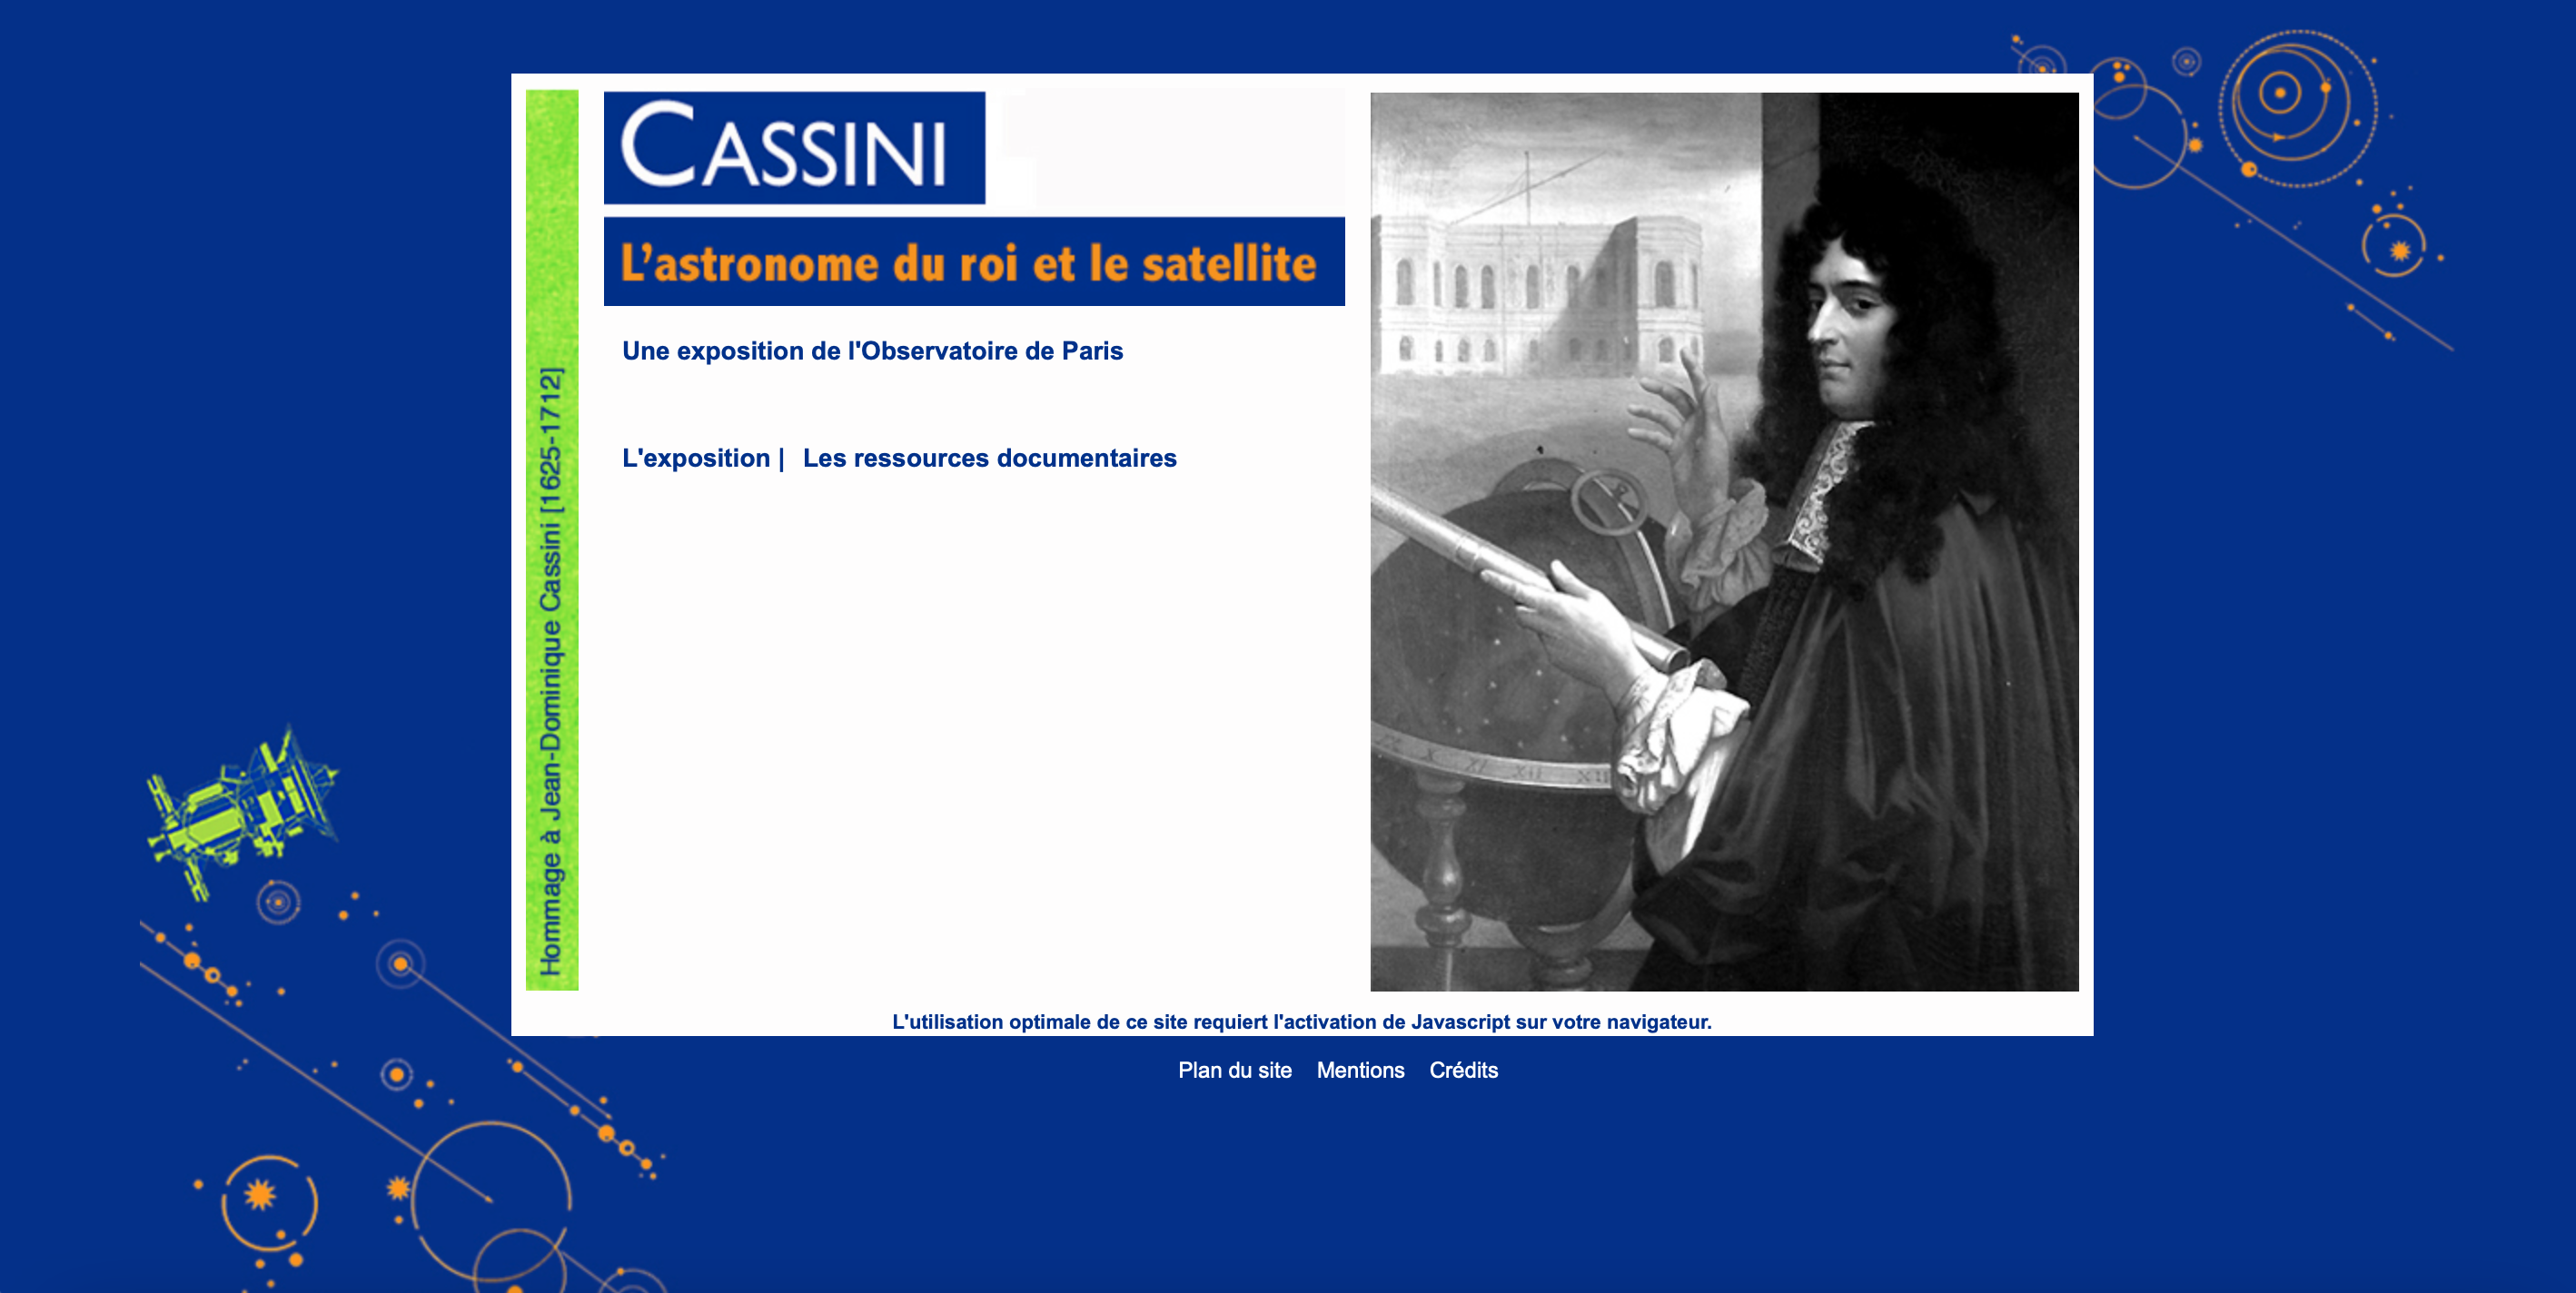
\includegraphics[scale=0.3, angle=0]{images/partie1/expositions/expo-cassini.png}
    \centering
    \end{figure}
	Cette exposition dont la scénographie a fait l'objet du stage de Loriane Buffet en 2012 a été conçue à l'occasion du tricentenaire de la mort de Jean-Dominique Cassini \footnote{\cite{buffetHommageJeanDominiqueCassino2012}. L'exposition peut quant à elle toujours être visitée \href{http://expositions.obspm.fr/cassini/index.php}{ici}.}. Elle accompagne une exposition montée physiquement dans les locaux du bâtiment Perrault de l'Observatoire de Paris (bibliothèque et salle Cassini). Ainsi, elle correspond à un type d'exposition virtuelle différent mais pouvoir avoir accès à un projet précédent au sein de le même institution est tout de même utile. De plus, il est aussi intéressant de remarquer les changements entre l'interface de cette exposition il y a dix ans et ce qui doit être envisagé pour répondre aux attentes qui sont celles des visiteurs d'aujourd'hui. Cela montre aussi que les expositions, virtuelles ou non, sont des objets de leur temps et le reflet des exigences scénographiques alors en vigueur. Les expositions physiques sont limitées dans le temps et l'espace tandis que les expositions virtuelles ne le sont \textit{a priori} pas. Néanmoins, même si elle perdure, l'exposition peut rapidement ne plus satisfaire et devenir, elle aussi, un objet limité dans le temps. Ainsi, la visite de cette exposition sur Cassini peut inviter à se questionner sur la pérennité de ce type d'objet. 
	
	\subsubsection{\textit{Le monde en sphères} à la \acrlong{bnf}}
	\begin{figure}[h]
	\caption{Page d'accueil du site de l'exposition \textit{Le monde en sphères}}
	\includegraphics[scale=0.3, angle=0]{images/partie1/expositions/expo-monde-en-spheres.png}
    \centering
    \end{figure}
	Cette, magnifique, exposition peut,  tout en restant réaliste, représenter une sorte d'objectif en terme de rendu visuel. Réalisée en 2019, elle vient elle aussi accompagner une exposition \textit{in situ} à la \acrshort{bnf} François-Mitterrand. Outre son aspect visuel, l'exposition de la \acrshort{bnf} a pu être une source d'inspiration pour la richesse des pages annexes au contenu principal et notamment la page \textit{Repères}. Ce glossaire est une addition très utile pour aider les visiteurs dans leur navigation en expliquant en quelques mots des notions parfois difficiles et méconnues. De façon analogue, une page \textit{Portraits de savants} est également présente et propose aux visiteurs de courtes biographies de certaines figures majeures pour l'histoire des sciences. Ces guides sont indispensables pour permettre aux visiteurs d'avoir tous les codes en main pour saisir au mieux ce que les auteurs ont cherché à montrer.

	Du fait de sa thématique, elle est proche de l'exposition du projet \acrshort{alfa}. Si la période couverte est plus longue et les objets exposés plus variés, des points de rencontre existent notamment dans la troisième partie intitulée \textit{La sphère dans l'Occident médiéval}. Cela montre que les expositions ne sont pas isolées et qu'elles doivent être replacées dans un contexte global de valorisation de documents manuscrits et de vulgarisation de contenu scientifique. Sur la page d'accueil du site, certains documents à voir absolument sont proposés au sein d'un parcours \textit{En bref} : ce sont les images qui frappent le plus le visiteur, les textes sont là en soutien, pour guider si besoin mais ils ne sont pas le cœur du sujet. La mise en valeur des documents se manifeste aussi par l'existence d'une banque d'images sur le site qui recense l'ensemble des images exposées et permet au visiteur qui le souhaite d'en apprendre plus sur un des documents par un simple clic. À partir de là, le visiteur a également la possibilité de consulter l'image, et le manuscrit dont elle est issue le cas échéant, sur Gallica. C'est ce type de contenu qui est aussi attendu pour l'exposition \textit{Medival skies under(book)cover}.
	
	\subsubsection{\textit{The art of reasoning in medieval mansucripts} à l'Académie royale néerlandaise des arts et des sciences}
	\begin{figure}[h]
	\caption{Page d'accueil du site de l'exposition \textit{Cassini, l'astronome du roi et le satellite}}
	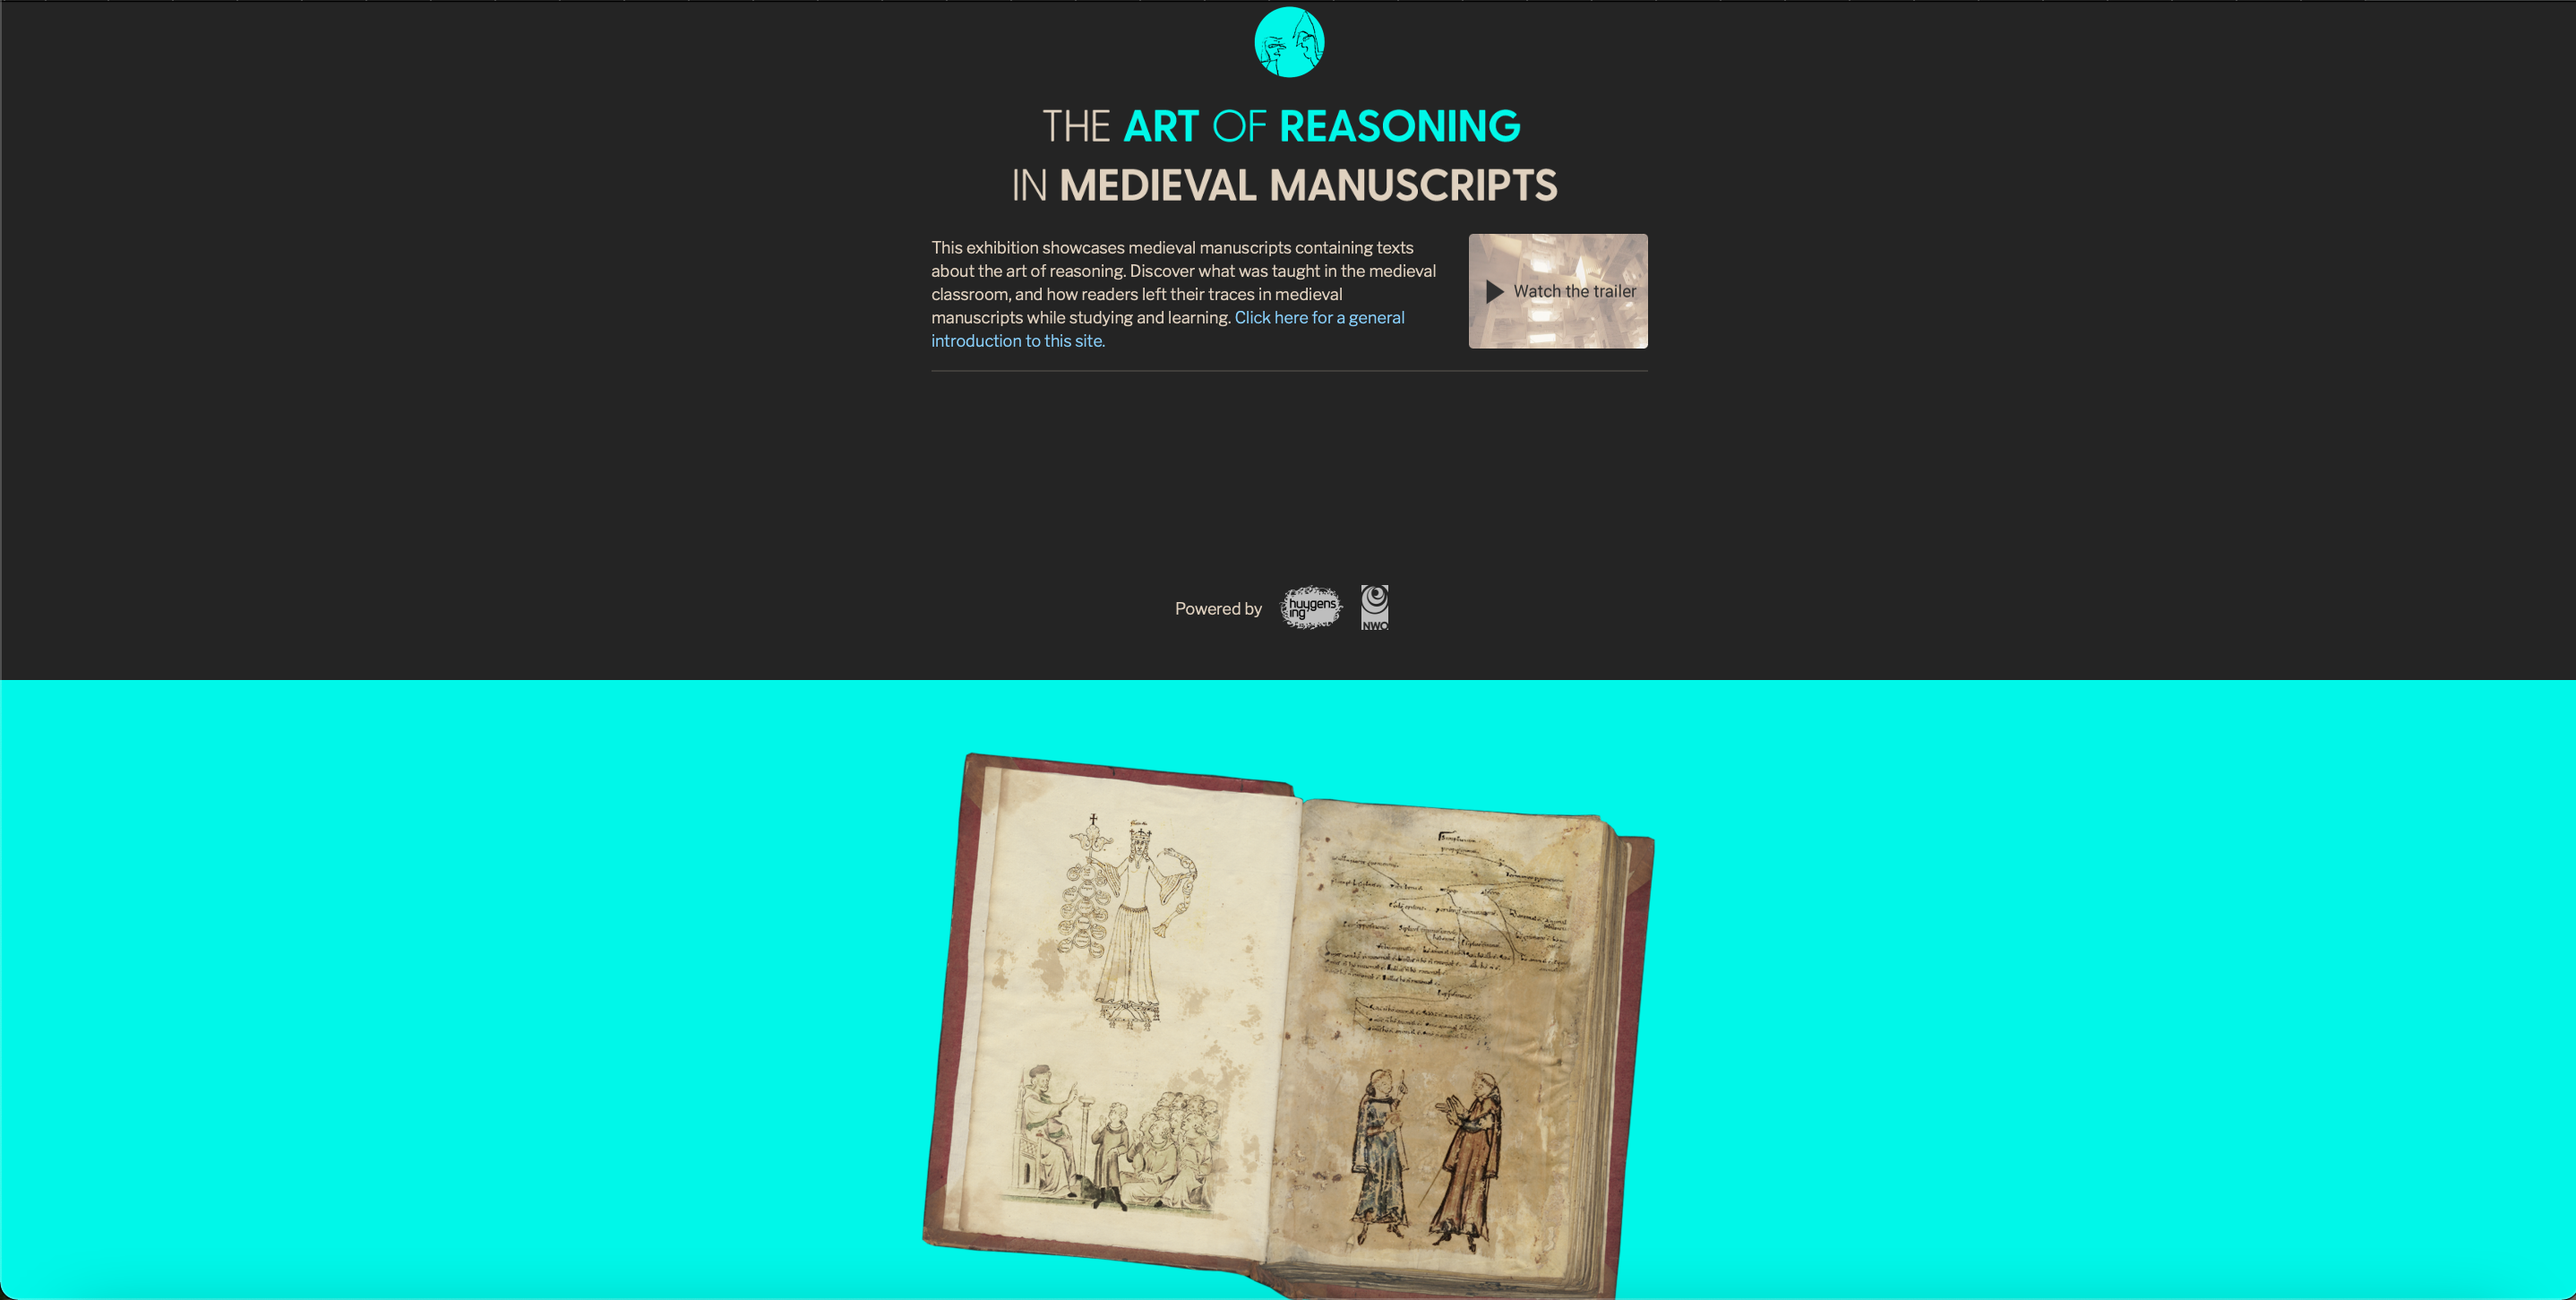
\includegraphics[scale=0.3, angle=0]{images/partie1/expositions/expo-art-of-reasoning.png}
    \centering
    \end{figure}
    Dernière exposition présentée ici, \textit{The art of reasonin in medieval mansucripts} est une exposition néerlandaise conçue dans le cadre du projet de recherche \textit{The Art of Reasoning: Techniques of Scientific Argumentation in the Medieval Latin West (400-1400)} financé de 2016 à 2020 par le Conseil néerlandais de la recherche. Le contexte de réalisation est donc très similaire à celui de l'exposition liée à ce stage. Le site est simple mais plutôt efficace avec quelques efforts pour rendre la navigation un peu interactive. Ainsi, le manuscrit de la page d'accueil est divisé en quatre parties cliquables qui donnent chacune accès à l'un des parcours de navigation du site. Un accès à chacun des manuscrits présentés est également possible via une page dédiée. Pour chaque manuscrit, le lecteur peut ensuite trouver des informations plus précises. C'est de cette exposition que vient l'idée d'une page d'accueil interactive pour l'exposition \acrshort{alfa}. Cela permet d'engager le visiteur et de lui faire prendre en main sa navigation dès son arrivée sur le site. 
    
    À travers les exemples de ces trois expositions, on peut avoir une idée de certains des enjeux liés à ce type de publication allant des simples considérations visuelles à des questions liées à la pérennité. \\
    
    Cette première partie a permis de poser les bases de ce mémoire en évoquant les éléments qui ont également été la base de mon stage. En effet, il était indispensable de cadrer le sujet en présentant le projet \acrshort{alfa} et les documents choisis par l'équipe pour figurer dans l'exposition et en définissant ce qu'est une exposition virtuelle. Une fois cela fait, il est désormais possible de poursuivre en s'intéressant plus concrètement à la scénographie de l'exposition \textit{Medival skies under(book)cover}.
	
	\part{Scénographie d'une exposition virtuelle}
	
	\chapter{Les parcours de l’exposition}
	Pour débuter, il convient de dire quels sont les différents parcours retenus pour naviguer au sein de l'exposition puis d'évoquer la manière dont les liens entre lesdits parcours sont envisagés.
	
	\section{Présentation des parcours}
	\subsection{Parcours patrimoine - \textit{Sensing}}
	Les parcours relatifs aux aspects patrimoniaux sont au nombre de 7, ils sont regroupés sous le nom de \textit{Sensing} au sein de l'exposition. Ces différents parcours se concentrent donc la matérialité des manuscrits (les manuscrits que l'on touche), sur des détails d'ordre visuel (les manuscrits que l'on voit) ou intellectuel (les manuscrits que l'on lit). 
	
	\subsubsection{\textit{Touching the manuscript: the material dimension of the corpus}}
	C'est la dimension matérielle des manuscrits qui est mise en avant dans ce parcours : la reliure ou bien la composition en cahier par exemple. L'un des buts est de souligner la complexité du livre manuscrit, en comparaison avec celle d'un livre imprimé. Il s'agit aussi de montrer comment les figures historiques présentent dans l'exposition utilisaient cette complexité au service de leurs travaux. 
	
	\subsubsection{\textit{Seeing manuscript: the visual dimension of the corpus}}
	Ici ce sont les principaux éléments visuels qui sont mis en valeur : mise en page, enluminures, décorations et illustrations, dispositif de lisibilité (ponctuation), diagrammes ou encore format des tables. C’est la richesse visuelle de ces documents qui est présentée aux visiteurs.

	\subsubsection{\textit{Student manuscript}}
	Produit dans un milieu universitaire par des étudiants, ces manuscrits peuvent être considérés comme des cahiers de cours. Bien que visuellement moins attractifs que d'autres au premier regard, ces manuscrits sont plus vivants avec notamment de nombreuses notes en marge indiquant des interventions des étudiants. Ils renseignent notamment sur l'organisation du cursus universitaire et sur les associations faites entre différentes disciplines : ainsi l'astronomie est souvent associée à d’autres disciplines mathématiques telles que l'optique, la géométrie ou l'arithmétique mais aussi parfois à des textes de médecine voire même de théologie. Certains de ces manuscrits d’étudiants ont appartenu à des acteurs majeurs dans l’histoire de l’astronomie alphonsine comme Conrad Heingarter par exemple.

	\subsubsection{\textit{University manuscript}}
	Ces manuscrits sont majoritairement produits au XVe siècle dans le milieu des universités. Le plus souvent, ils sont produits dans le cadre de la \textit{peccia} qui est un système qui permettait à plusieurs copistes de recopier en même temps un ouvrage, ce système s'est développé avec la nécessité de fournir aux étudiants les textes indispensables à leurs études, ces manuscrits constituent ainsi des sortes de manuels. Certains de ces manuscrits peuvent aussi être réalisés dans des ateliers spécialisés. Selon leur contexte de fabrication, ils peuvent être plus ou moins précieux. 

	\subsubsection{\textit{Presentation manuscript}}
	Ces manuscrits sont, en général, produits par des ateliers spécialisés où l'on trouve à la fois des copistes, des miniaturistes, des enlumineurs, etc.. Il en existe deux principales sortes. Les premiers sont directement produits par des cours pour en assurer le prestige intellectuel, pour la tradition alphonsine c'est le cas de la cour d'Alphonse X ou de celle de Charles V \footnote{Né en 1338 et mort en 1380, il est roi de France à partie de 1364.}. Ils peuvent faire l'objet de présents diplomatiques ou de prise de guerre. Les autre sont produits par des savants qui les destinent à des personnages riches et puissants susceptibles de leur accorder leur protection. 

    Ce sont de très beaux manuscrits, d’une grande valeur patrimoniale, qui permettent de mieux saisir le contexte dans lequel se développe alors l'astronomie qui n'est pas restreinte aux seuls cercles scientifiques mais connaît un développement social et culturel bien plus large. Là encore, certains des manuscrits présentés dans l'exposition ont appartenu à des figures historiques d'importance première pour l'astronomie alphonsine. 

	\subsubsection{\textit{Toolbox manuscript}}
	Ces manuscrits qui constituent la quatrième grande catégorie de manuscrits présents dans l'exposition sont des documents véritablement issus de la pratique de l'astrologie. En effet, ils sont produits par des astrologues lorsque ceux-ci se consacrent à leur activité et sont composés de leur outils de calcul. Certains sont spécialisés dans une question astronomique ou dans un outil tandis que d'autres ont vocation à être plus généralistes et l'on pourra y trouve des textes, diagrammes ou tables portant sur différents sujets. 
	
	\subsubsection{\textit{Exceptional manuscript}}
	Si tous les manuscrits présentés dans cette exposition sont à leur manière exceptionnels, ceux de cette catégorie le sont encore davantage. Certains ont une organisation codicologique particulière, c'est le cas du \textit{batbook}, très peu de manuscrits de ce type subsistent encore, ce qui les rend encore plus précieux. D'autres font figure d'exception par ce qu'ils contiennent : uniquement des instruments, une "histoire" de l'astronomie par les textes ou encore des autographes de Regiomontanus, Jean de Saxe ou Jean de Murs.

	\subsection{Parcours historique - \textit{Learning}}
	On peut distinguer plusieurs étapes dans le développement de l'astronomie alphonsine à travers d'abord des origines en al-Andalus en lien avec les traditions arabes, vient ensuite un moment parisien avec le passage au latin. Après cela, le corpus parisien a voyagé ailleurs en Europe où de nouveaux textes ont vu le jour. L'ultime étape intervient à la fin de la période et correspond à l'amorce d'une transition vers le monde de l'imprimé. 

	\subsubsection{\textit{Royal origins in al-Andalus}}
	En se plaçant à la cour d'Alphonse X, ce parcours vise à mettre en lumière les origines de l'astronomie alphonsine et ses liens avec l'astronomie arabe. Ce parcours s'appuie donc en majorité sur des manuscrits produits à la cour d'Alphonse X mais également sur d'autres s'ils contiennent des éléments issus de la tradition des tables de Tolède, d’Al-Khwarizmi ou d’Al-Battani.

	\subsubsection{\textit{Paris University}}
	Dans ce parcours, l'accent est mis sur l'étape parisienne de l'histoire de l'astronomie alphonsine et sur les œuvres de Jean Vimond, Jean de Lignères, Jean de Saxe et Jean de Murs qui ont participé à une première diffusion latine de l’astronomie alphonsine.
	
	\subsubsection{\textit{Fostering astronomical activities around Europe}}
	Le but de ce parcours est de montrer comment l'astronomie alphonsine s'est étendue à d'autres horizons européens en proposant aux visiteurs de s'intéresser à des manuscrits et des œuvres produits en Angleterre, en Italie ou en Europe centrale.  
	
	\subsubsection{\textit{Transition to the printing world}}
	Dans ce dernier parcours, il s'agit de se placer à la fin du XVe siècle quand des cercles humanistes ont assuré les premières impressions de textes issus du corpus alphonsins, Bianchini, Regiomontanus ou Peurbach par exemple.
	
	\subsection{Parcours scientifique - \textit{Understanding}}
	Les parcours de ce thème ont pour objectif de familiariser les visiteurs avec le contenu scientifique des manuscrits alphonsins. Par contenu scientifique, il faut entendre ici les phénomènes astronomiques étudiés aussi bien que les outils mathématiques indispensables à ces études. 
	
	\subsubsection{\textit{Spherical astronony}}
	C'est un type d'astronomie qui s’intéresse au lever et coucher des astres, aux différentes longueurs du jour et de la nuit selon la période de l’année et la latitude, aux ombres etc. C’est une partie essentielle de l’astronomie, elle permet notamment de déterminer l’ascendant, point clé de toutes prédictions astrologiques. L'objectif de ce parcours est de fournir aux visiteurs des notions de base sur cette astronomie en s'appuyant sur les manuscrits exposés et les outils qu'ils renferment. 

	\subsubsection{\textit{Planetary astronony}}
	À l'image du précédent, ce parcours donnera des notions de bases sur un autre type d'astronomie qui étudie la manière dont les mouvements en longitude et en latitude des planètes étaient modélisés et calculés. L'objectif est ici de montrer comment les textes, diagrammes et tables sont utilisés dans ce cadre.
	
	\subsubsection{\textit{Eclipse}}
	Là encore, en s'appuyant sur les manuscrits, ce parcours accompagnera les visiteurs verts la découverte de notions de base au sujet des éclipses. C'est le dernier parcours lié à un type d'astronomie en particulier.
	
	\subsubsection{\textit{Diagrams and instruments}}
	Ce parcours, comme les suivants, se concentre sur un outil intellectuel utilisé par les astronomes médiévaux pour étudier les phénomènes astronomiques plutôt qu'à un phénomène en particulier. Ici, on propose aux visiteurs de s'intéresser aux diagrammes et la manière dont ils sont utilisés. Certains de ces diagrammes sont en fait des instruments, parfois même des instruments de calculs.

	\subsubsection{\textit{Astronomical tables}}
	De la même manière, on souhaite ici attirer l'attention des visiteurs sur les tables et sur certaines des valeurs significatives qu’elles contiennent. Un autre point d'attention est le type de nombres utilisés.

	\subsubsection{\textit{Texts}}
	Dans ce dernier parcours lié à un type d'instrument, on présente aux visiteurs les différents types de textes présents dans le corpus alphonsin et la manière dont ils contribuent à mettre en mouvement et en relation les tables et les diagrammes.

	\subsubsection{\textit{Other disciplines}}
	Ultime parcours de cette section dédiée aux éléments scientifiques, ce parcours s'attache à montrer les liens qui existent, notamment dans le milieu universitaire, entre l'astronomie et d'autres sciences : autres disciplines mathématiques, médecine ou théologie.
	
	\subsection{Parcours manuscrits - \textit{Reading}}
	L'intégralité des manuscrits ayant été présentée dans le chapitre 2, les parcours relatifs à chacun d'entre eux ne seront pas détaillés une nouvelle fois. Il importe simplement de dire qu'un parcours est prévu pour chacun des quinze manuscrits, ces parcours permettront aux visiteurs de saisir la richesse qu'ils contiennent.

	\section{Matrice et \textit{deep linking}}
    Tous les parcours précédemment présentés peuvent fonctionner individuellement mais ils ne sont pas dépourvus de lien les uns par rapports aux autres. En effet, il est aisé de constater que ceux relatifs à un même thème peuvent être considérés comme les différentes parties d’un même parcours bien plus étendu mais d’un thème à l’autre il existe aussi des ponts notamment rendus possibles par la richesse de contenu des manuscrits : un manuscrit appartient souvent à plusieurs parcours. De plus, certains \textit{attention points} peuvent, eux aussi, être communs à différents parcours. Pour mettre cela un peu plus au clair, un tableau de ces \textit{attention points} communs \footnote{Ce tableau est disponible en annexe \ref{APcommuns}, à la page \pageref{APcommuns}.} a été réalisé pour venir compléter celui déjà produit par les chercheurs pour garder une trace de la répartition des \textit{attention points} au sein des divers parcours. Dans ce tableau, un code couleur simple est utilisé pour déterminer dans combien de parcours un \textit{attention point} peut être rencontré et des liens renvoient vers l’exacte position de cet \textit{attention point} dans chacun des parcours concernés. Ces liens précis sont essentiels pour la construction de l’exposition telle que l’équipe la souhaitait. En effet, l’idée n’est pas ici d’imposer aux visiteurs un unique sens de progression déjà tracé au sein de l’exposition. Au contraire, l’utilisateur, bien que guidé, est libre d’aller et venir entre les différents thèmes en commençant où bon lui semble. 
    
    Néanmoins, pour que chacun puisse prendre part à une visite complète de l’exposition, des pistes de poursuite de la navigation peuvent être suggérées. Ainsi, le visiteur peut être invité à une découverte plus approfondie des questions scientifiques après avoir visité le parcours ayant pour objet les manuscrits d’étudiants. Par ailleurs, pendant sa navigation au sein d’un parcours, le visiteur aura également la possibilité de changer de direction. Par exemple, si dans le parcours dédié aux tables astronomiques, un \textit{attention point} fait mention du manuscrit \acrshort{bnf} Mélanges Colbert 60, le visiteur aura la possibilité de bifurquer vers le parcours entièrement consacré à cet unique. Inversement, un visiteur qui serait en train de parcourir ce même manuscrit serait en mesure de se rendre vers le parcours relatif au moment parisien de l’astronomie alphonsine via un \textit{attention point} en faisant mention. 
    
    Certains des parcours envisagés par les chercheurs sont très longs et le temps à y consacrer dépasse nettement la quinzaine de minutes fixée au départ. Pour pallier les éventuels problèmes que cela pourrait engendrer, la solution suivante a été proposée : créer deux versions de ces parcours, une complète et une courte. Cette version raccourcie pourra satisfaire des visiteurs pressés et/ou novices en leur proposant de ne s’attarder que sur les pièces majeures du parcours. Pour ceux qui le souhaitent, à la fin de cette version réduite, l’accès à la version longue sera permis. Dans le même ordre d’idée, l’inclusion de \textit{must see} est également envisagée en s’appropriant l’approche de \textit{gateway object} décrite par les équipes du British Museum \footnote{\cite{battyObjectFocusedText2016}.} pour des expositions \textit{in situ} et en l’adaptant à une visite en ligne.  Il s’agit de désigner quelques objets représentatifs de l’ensemble et attractifs pour le visiteur qui pourra s’intéresser à chacun d’eux dans l’ordre de son choix et accéder à la fois aux principaux objets en tant que tels mais également, à travers eux, aux principales clés de compréhension de l’astronomie alphonsine. Qu’il s’agisse de la sélection de \textit{must see} ou de la création de certains parcours dans une version plus courte, le travail doit encore être poursuivi mais l’idée est là et des tests ont pu être réalisés pour leur mise en œuvre concrète sur le site de l’exposition. 
    
    En suivant toujours cette même logique de ne pas imposer d’unique manière d’appréhender cette exposition aux visiteurs, ce qui a en revanche déjà été implémenté est un affichage des parcours relatifs à un thème dans un ordre aléatoire sur la page dédiée. Cela souligne bien qu’il n’est pas nécessaire d’avoir visité un parcours pour en comprendre un autre, chacun peut être positionné où le visiteur le souhaite dans sa visite. Néanmoins, certains parcours sont plus accessibles que d’autres, ainsi pour un visiteur n’ayant peu ou pas de connaissances en astronomie, commencer par les parcours à caractères scientifiques pourrait rendre la progression plus difficile voire la stopper par perte d’intérêt devant la complexité de certaines notions. C’est pour cela que sans rien imposer, ces parcours arrivent en troisième position dans la barre de navigation : si le visiteur suit la progression ainsi suggérée, il aura déjà pu se familiariser avec les documents avant de s’engager dans les parcours les plus techniques. 

    Ainsi, cette exposition est conçue pour être une sorte de matrice ouvrant des possibilités multiples aux visiteurs qui peuvent choisir de se laisser pleinement guider par les chercheurs ou se laisser porter par leur propre curiosité. 

	
	\chapter{Analyse des besoins des publics}
	Vient à présent le temps de se consacrer de façon plus détaillée aux attentes des publics en précisant d'abord qui ils sont avant de s'engager dans quelques réflexions sur l'expérience qui doit être celle des utilisateurs et sur la fréquentation des expositions. 
	
	\section{Public(s) ciblé(s)}
    Certaines réflexions avaient déjà été portées en amont et quatre catégories de public avaient ainsi pu être déterminées : étudiants, chercheurs, professionnels du livre et une dernière catégorie bien plus large faisant référence à des visiteurs variés. Une première étape a été d’essayer d’établir quels pouvaient être les intérêts et les besoins de tous ces potentiels visiteurs. 
    Ainsi, pour les différents publics envisagés, il est apparu nécessaire de chercher à savoir quelles étaient leurs activités principales, où est-ce qu’ils travaillaient, par quels moyens seraient-ils être en mesure d’entendre parler de l’exposition, quelles pourraient être leurs attentes ? Il était également important de songer dès lors à des idées pour que lesdites attentes soient satisfaites. 

    \subsubsection{Les professionnels du livre}
    Viennent premièrement les professionnels du livre. On suppose qu’ils travaillent dans des bibliothèques ou des institutions patrimoniales et que c’est probablement sur leur lieu de travail qu’ils auront connaissance de l’exposition. Ils sont susceptibles d’être demandeurs d’informations bibliographiques précises, ce qui peut être fait en indiquant des ressources extérieures telles que les notices des manuscrits publiées sur les site web des institutions de conservation ou encore les pages wikipedia des manuscrits lorsqu’elles auront fait l’objet d’une mise en ligne. Un autre intérêts pour eux peut résider dans la mise en valeur de leurs propres collections. Néanmoins, cela ne constitue pas nécessairement une motivation pour visiter l’exposition mais sans doute plutôt pour y prendre part. 
 
    \subsubsection{Les chercheurs}
    À l’instar des précédents, les chercheurs constituent un public de professionnels ayant déjà acquis des connaissances sur au minimum une des principales thématiques de l’exposition : considérons donc ici les chercheurs dans les domaines de l’histoire des sciences ou de la codicologie par exemple. Leurs attentes sont donc plutôt portées vers des explications détaillées accompagnées de ressources extérieures permettant d’aller plus dans le détail encore. Si le renvoi vers des ressources extérieures est tout à fait envisageable, ce n’est pas forcément le cas des explications complexes puisque cela rendrait l’accès beaucoup plus difficile à d’autres types de publics. Or, le but de cette exposition étant de valoriser des manuscrits astronomiques, il semble essentiel que l’audience puisse être la plus large possible jusqu’à toucher des personnes tout à fait novices sur les thématiques proposées. 

    Ainsi, et également pour satisfaire d’autres besoins de ce projet, en particulier le temps à passer sur chacun des parcours, le choix a été fait de se focaliser sur une audience large qui chercherait à découvrir l’astronomie alphonsine plutôt que de s’adresser vraiment à des spécialistes. En effet, dès la conception de l’exposition l’idée était plutôt d’avoir des textes simples et idéalement assez courts permettant de saisir les éléments essentiels et non d’entrer dans des détails peu accessibles à une audience non spécialiste. Néanmoins, les spécialistes ne sont pas exclus. En effet, l’ajout d’une section bibliographique sur le site web de l’exposition autorise un accès à des informations bien plus précises et à des ressources extérieures apportant plus de détails. De plus, l’idée étant, \textit{in fine}, d’avoir à la fois des versions longues et des raccourcis, au moins pour les parcours les plus longs, un public spécialisé pourra également être davantage intéressé par ces versions longues.

    \subsubsection{Les étudiants}
    Au sein de cette audience plus large finalement désignée comme public cible, il est possible de détacher un groupe particulier : les étudiants qui sont un public très éclectique, demandeur à la fois de contenu éducatif avec des exemples concrets et d’éléments plus ludiques. Cela en fait un public tout à fait intéressant pour une exposition en ligne. En effet, l’aspect interactif et immersif est propice à capter l’attention et à la maintenir plus longtemps. Par ailleurs, une telle exposition peut potentiellement être utilisée comme un support d’illustration par des professeurs ou parents dans le cadre du parcours scolaire. 

    \subsubsection{Un large public}
    En choisissant un public de visiteurs variés plutôt qu’un groupe précis comme public cible, l’équipe en charge de l’exposition est consciente qu’il sera difficile de répondre à des attentes aussi variées que le sont les visiteurs. Néanmoins, il est possible de mettre en avant certains souhaits communs, à commencer par la volonté de découvrir et d’en apprendre davantage sur l’astronomie ou sur les manuscrits. Ce public peut également être tout simplement désireux de porter un regard nouveau sur le Moyen Âge.  À l’image des étudiants, ce public novice peut aussi être friand et demandeur d’une dimension ludique. Aussi, une section de jeux a été envisagée, bien que celle-ci ne soit pas encore implémentée. 
    Néanmoins, face à un public si large, il n’est pas possible de cerner parfaitement les besoins et par conséquent de satisfaire les attentes de tous les éventuels visiteurs. Par ailleurs, si l’on veut vraiment inclure ce public le plus large possible, il est essentiel de garder en tête que si le numérique peut attirer, il peut aussi représenter un frein pour d’autres. Un plan du site ou bien un guide d’utilisation mériteraient donc d’être ajoutés. 

	\section{Expérience utilisateur}
	Pour répondre au mieux aux diverses attentes précédemment évoquées, des réflexions sur l’\textit{UX design} peuvent se révéler très utiles. 				\og{} L’expérience utilisateur est une forme spécifique d’expérience humaine qui naît de l’interaction avec une technologie ou un service. Le design UX a pour objectif de rendre cette expérience la plus positive possible en la pensant avant le produit\fg{} \footnote{\cite{gronierMethodesDesignUX2017a}.}. L ‘utilisateur est donc au cœur du processus de développement. Le produit en tant que tel ne se suffit plus à lui-même et l’expérience qui sera celle de l’utilisateur a toute son importance. Pour définir au mieux, les besoins de ces futurs utilisateurs, la méthode des personas peut-être utilisée. C’est un outil qui peut être défini ainsi : 

    \begin{quote}
	    Les personas [permettent] de produire des connaissances sur l’utilisateur, connaissances pouvant aider les concepteurs à développer des fonctionnalités utiles à la conception d’applications informatiques innovantes \footnote{\cite{brangierEffetsPersonasContraintes2012}.}. 
    \end{quote} 

    C’est un outil qui est de plus en plus utilisé et intégré dans les phases de conception d’objets numériques. S’il présente de nombreux avantages et permet de considérer de manière plus importante les utilisateurs, c’est un outils imparfait qui s’appuie en partie sur des idées préconçues sur le(s) public(s) ciblé(s). 


    Cette expérience utilisateur n’est pas qu’une question de rendu esthétique final, il s’agit aussi de prendre en compte les exigences du public en terme de navigation. Comme cela a été mentionné, le public ciblé cherche à découvrir de nouvelles choses mais sans que cela ne paraisse rébarbatif. Pour cela, la navigation se doit d’être fluide et intuitive. De plus, le temps passé sur chacun des parcours ne doit pas excéder une quinzaine de minutes afin de maintenir les visiteurs attentifs et captivés. L’utilisateur doit constamment être engagé et se sentir maître de sa déambulation au sein de l’exposition : il est le narrateur de l’histoire qu’il visualise. Les personnes en charge du développement du site web se doivent donc prendre cela en considération et faire en sorte que le visiteur puisse avoir accès à une véritable expérience. Les enjeux doivent être clairs et s’ils ne le sont pas, ils doivent être accompagnés d’explication. : cela participe au confort des visiteurs qui constitue l’un des points essentiels des réflexions sur l’\textit{UX design}. Il en va de même pour les éléments de navigation qui ne seraient pas intuitifs. Un plan du site peut s’avérer être une addition non négligeable pour permettre aux visiteurs d’avoir une idée d’ensemble de ce qui leur est proposé au sein de l’exposition. Quoi qu’il en soit, l’image doit être première au sein de l’exposition : elle doit faire sens et séduire le visiteur.

    \section{Fréquentation des expositions}
    L’exposition est une forme de médiation qui rencontre le plus souvent son public. En effet, les expositions à succès ne sont pas des faits rares, notamment dans le monde muséal. Les expositions conçues par les équipes de grandes bibliothèques telles que la \acrshort{bnf} connaissent aussi un vif succès et dans le cas de la \acrshort{bnf}, les documents mis en valeur peuvent être similaires à ceux mis en scène dans l’exposition \textit{Medieval skies under(book)cover}, cela prouve l’existence d’un public pour ce type d’opération de valorisation. 

    Comme le rapporte le Ministère de la Culture le 26 juin 2020, la pandémie de Covid-19 a marqué un changement important pour la fréquentation en ligne des collections patrimoniales. En effet, qu’il s’agisse des collections elles-mêmes ou des pages qui recensent ces mêmes collections, les chiffres ont été grandement multipliés : par exemple, la page du site Musées \footnote{\cite{ministeredelacultureetdelacommunicationChiffresClesStatistiques2021}.} où sont indiquées les expositions virtuelles a vu sa fréquentation augmenter de 2000\%. Le Ministère indique aussi que 
    \begin{quote}
    Même s’il est prévisible que ces chiffres baisseront après la réouverture des musées, certains internautes, séduits par la qualité des contenus, continueront de fréquenter les sites Internet des musées. 
    \end{quote}
    Si la note vaut pour les musées, une tendance similaire est observable pour la \acrshort{bnf}. En effet, en 2021, la fréquentation de Gallica a diminué de 2\% par rapport à 2020 mais en comparaison à 2019, elle est supérieure de 19\%. Cela montre bien que même si le contexte du confinement était particulier, certaines habitudes prises se maintiennent notamment en terme de consommation de la culture. C’est un paramètre à prendre en compte lors du développement d’une exposition en ligne. Ainsi, on peut supposer que le succès de l’exposition conçue pour le projet \acrshort{alfa} sera plus important que ce qu’il aurait pu être il y a quelques années du fait de ces nouvelles habitudes. C’est aussi l’une des raisons qui peut justifier de s’adresser à un large public pour cette mise en valeur de manuscrits astronomiques. Toutefois, pour garder vivante cette consommation en ligne, les données proposées aux visiteurs doivent l’être selon des modalités qui en plus de les mettre en valeur les rendent attractives aux visiteurs.
	
	\chapter{Gestion de projet}
	Parmi les missions confiées au cours de ce stage figurent des tâches relatives au suivi et à la gestion du projet au cours de différentes phases de développement. Seront évoquées tour à tour la question du dialogue avec les chercheurs et  celle de la rédaction de documentation.
	
	\section{Dialogue avec les chercheurs}
	\subsection{Intermédiaire entre ingénierie et recherche}
	Dans le cadre d'un projet de recherche, le dialogue est primordial pour coordonner les avancées et répartir le travail à effectuer. Ici, le dialogue doit aussi se faire entre les chercheurs et les ingénieurs, chacun est engagé dans le projet mais avec des missions à la fois différentes et complémentaires. Le rôle qui a été le mien était celui d'intermédiaire. En effet, il s'agit d'identifier, de comprendre et d'analyser les besoins des chercheurs tout en ayant des connaissances de la réalité du terrain qui permettent de mettre en perspective ces besoins et de se questionner sur leur faisabilité. C'est aussi l'occasion d'avoir un point de vue plus englobant prenant en compte les différents besoins et positions de chacun. Il faut donc faire preuve d'analyse et de synthèse pour garder à l'esprit les objectifs du projet et mettre en œuvre les solutions qui semblent les plus adaptées pour y parvenir. 
	
	Si recherche et ingénierie sont souvent perçues comme deux disciplines que l'on ne peut réunir, les humanités numériques, dont la place est grandissante, sont une preuve qu'un dialogue est possible et surtout bénéfique à l'un et l'autre de ces milieux. Cette dichotomie est assez caractéristique du paysage universitaire français \footnote{\cite{foucherAtlasInfluenceFrancaise2013}, p. 44}. Le développement de rapprochements entre ces deux sphères permet aux ingénieurs de mettre leurs compétences techniques au service des sciences humaines tandis que les chercheurs peuvent bénéficier d'outils qui leur étaient jusqu'alors inaccessibles mais qui se révèlent utiles pour leur travaux. Les possibilités permises et horizons ouverts ne cessent de croître par la présence plus visible de projets interdisciplinaires. C'est le cas du projet \acrshort{alfa} où histoire des sciences et valorisation numérique sont intrinsèquement liées. La présence sur place d'une \textit{\acrshort{dh} team} souligne cela. Tous les lundis un point hebdomadaire est fait sur le travail réalisé au cours de la semaine passée et sur les objectifs pour la semaine à venir pour les membres de cette petite équipe. Ces réunions ont lieu avec Matthieu Husson, chef du projet de recherche \acrshort{alfa}, et Ségolène Albouy, cheffe de projets numériques. Ces rendez-vous sont aussi l'occasion de discuter des idées et ainsi statuer sur celles qui sont à explorer et celles qui sont à exclure. 
	
	\subsection{Séminaires DH}
	Des temps d'échange avec l'ensemble de l'équipe sont également prévus notamment par le biais de séminaires internes à l'équipe et ayant pour objet les \acrlong{dh}. Lors de ces séminaires, des outils informatiques peuvent être présentés mais ils peuvent aussi être l'occasion pour l'équipe en charge de l'ingénierie de présenter son travail aux chercheurs. Pour des projets réellement communs comme cette exposition, ce séminaire est un moment important d'échange et de réflexion. Au cours de mon stage, trois séminaires \acrshort{dh} ont eu lieu : le premier, animé par Ségolène Albouy, présentant le protocole \acrshort{iiif} et les deux autres relatifs à l'exposition et que j'ai pu préparer et présenter, accompagnée de la cheffe de projet numérique. 
	
	Le premier a eu lieu en mai et le but était alors de faire un point sur les ressources à disposition au début du stage et de poser les questions qui étaient les miennes à propos de ces dernières, de présenter à l'ensemble de l'équipe, chercheurs et ingénieurs, des idées de scénographie et de proposer d'utiliser Exhibit plutôt que Storiies Editor. Les riches discussions survenues au cours de ce séminaire ont grandement participé aux réflexions alors en cours relatives à la scénographie et à l'expérience qui doit être celle des visiteurs. L'éventuelle création de versions écourtées pour les parcours les plus longs a notamment été évoquée lors de ce séminaire, de même que la question du titre à donner à l'exposition. 
	
	Le second a, quant à lui, eu lieu en juillet donc à un stade plus avancé du stage. La première partie a été consacrée à une présentation du site de l'exposition tel qu'il était alors : en construction. Cela a permis de réfléchir ensemble aux ajouts à faire et aux éléments à améliorer. De plus, ce séminaire a donné l'occasion de faire un point sur les manuscrits sélectionnés pour apparaître dans l'exposition et sur les modalités de communication pour ceux qui n'étaient pas numérisés ou alors dont la numérisation n'était pas libre de droit. La deuxième partie du séminaire s'est déroulée sous forme de \textit{workshop} pour permettre aux chercheurs de prendre en main l'outil Exhibit avec la possibilité d'être guidés et d'obtenir une réponse immédiate à leurs éventuelles questions. La préparation de ce séminaire a donné lieu à la rédaction de documentation relative à Exhibit pour également fournir aux chercheurs un document écrit auquel se référer. Celui-ci a pu être complété suite aux questions posées au cours du \textit{workshop} \footnote{Les présentations utilisées en support de ces deux séminaires sont disponibles en annexe \ref{Séminaires}, à la page \pageref{Séminaires}.}.

	\section{Rédaction de documentation}
	\subsection{À destination des chercheurs}
	Comme mentionné juste au dessus, au cours de mon stage j'ai eu l'occasion de rédiger de la documentation adressée avant tout aux chercheurs. Le projet et l'équipe étant internationaux, l'ensemble des documents a été rédigé en anglais. La principale documentation à destination des chercheurs est un tutoriel pour réaliser des \textit{exhibits} grâce à l'outil du même nom \footnote{Ce document a été reproduit tel quel, donc en anglais, en annexe \ref{Tutoriel}, à la page \pageref{Tutoriel}.}. Ce document propose treize étapes qui doivent permettre de construire ou de modifier un parcours de l'exposition, selon les règles qui ont été discutées avec l'ensemble de l'équipe au cours du \textit{workshop}. Les treize étapes sont les suivantes : 
	\begin{enumerate}
    \item Trouver ou créer un \textit{exhibit}
    \item Définir les paramètres
    \item Ajouter un \textit{manifest} à l'\textit{exhibit}
    \item Rédiger une \textit{caption}
    \item Ajouter des questions
    \item Ajouter des \textit{pinpoints}
    \item Traduire et harmoniser l'utilisation de l'italique et des guillemets 
    \item Changer l'ordre des \textit{attention points} d'un parcours
    \item Trouver des titres
    \item Ajouter des liens dans les \textit{captions}
    \item Dupliquer un \textit{exhibit}
    \item Rédiger ou compléter les \textit{attention points}
    \item Conserver les liens 
    \end{enumerate}

    Toutes ces étapes ne sont pas obligatoires à chaque fois, cela dépend du parcours sur lequel le chercheur est en train de travailler. Si certains de ces éléments seront détaillés davantage dans le chapitre suivant, ce n'est pas le cas de tous et ceux dont il ne sera plus questions vont donc faire l'objet de quelques précisions dès maintenant. Les manuscrits exposés sont des manuscrits en latin, or on peut supposer que l'intégralité des visiteurs ne sera pas pleinement confortable avec la lecture de cette langue. Ainsi, toutes les citations latines doivent être traduites en respectant ces règles : la citation latine est retranscrite entre guillemets tandis que sa traduction est ajoutée entre parenthèses. Les titres sont quant à eux donnés en italique. Définir ces règles simples permet une harmonisation à l'échelle de l'exposition alors que différentes pratiques pouvaient être observées du fait des différentes mains ayant pris part à la rédaction des \textit{attention points}. Un autre point à expliciter est le numéro 8. Cela concerne notamment les parcours thématiques. En effet, à l'intérieur de ces parcours les \textit{attention points} ont été insérés dans les \textit{exhibits} manuscrit par manuscrit, ce qui n'est pas une solution optimale pour capter l'attention des visiteurs. Une progression thématique mélangeant les différents manuscrits est à privilégier. Concernant le point numéro 9, certains \textit{attention points} s'étaient vus attribuer des titres, là encore selon la personne qui a procédé à leur rédaction. C'est une bonne idée qui aiderait les visiteurs à se repérer dans l'exposition et trouver des titres pour les \textit{attention points} n'en disposant pas encore serait une manière d'améliorer les \textit{exhibits}. Enfin, pour certains manuscrits la totalité ou une partie des \textit{attention points} ne sont pas rédigés et il conviendrait donc d'y remédier.

    En complément de ce document, d'autres relatifs aux \textit{exhibits} ont été produits : un tableau récapitulatif de tous les \textit{attention points} communs à plusieurs parcours \footnote{Déjà évoqué,ce tableau récapitulatif est disponible en annexe \ref{APcommuns}, à la page \pageref{APcommuns}.} et un autre, qui, pour chaque figure historique mentionnée, indique le folio et donc l'\textit{exhibit} concerné en fournissant le lien, les liens vers les ressources telles que Biblissima et Wikipedia sont également indiqués.

	\subsection{À destination d'ingénieurs}
	Une documentation avec un caractère plus technique et donc davantage destinée à des ingénieurs a également été rédigée avec en premier lieu l'élaboration d'un document de spécifications. Ce document vise à lister le contenu des pages du site web, les liens qui devront être disponibles sur chacune de ces pages mais également les éléments à vérifier pour le fonctionnement. Ce document permet d'avoir une base des attentes à laquelle se référer dans toutes les étapes ultérieures du développement du site web. S'il peut aussi être utile aux chercheurs, ce document présente un véritable intérêt pour de futurs développeurs chargés de compléter le site de l'exposition en y ajoutant notamment les pages envisagées mais pas encore implémentées : ils auront alors accès aux informations nécessaires concernant la place de ces pages dans l'architecture globale du site web et le contenu qui doit être le leur \footnote{Ce document a été réalisé après avoir analysé les différentes ressources à disposition et avant d'entamer la phase de réalisation, il peut être consulté en annexe \ref{Spécifications}, à la page \pageref{Spécifications}}. 
	
	Outre cela, une documentation du code de l'application est également disponible sur le \textit{repository} du projet d'exposition, accessible sur le GitLab de l'Observatoire de Paris. Git est un outil de \textit{versionning} qui permet le développement informatique à plusieurs mains en travaillant sur différentes branches. La possibilité d'accéder à des versions antérieures du projet peut constituer en soi une forme de documentation. Néanmoins, la véritable documentation accessible via GitLab correspond aux Wikis qui ont été rédigés. Ils contiennent des informations relatives à l'installation de l'application mais pas seulement. Toutes sortes d'éléments y sont décrits qui doivent être en mesure de permettre à d'autres ingénieurs, plus tard dans ce même projet ou pour un autre projet, de comprendre l'arborescence des dossiers ou encore de savoir quels sont les changements à effectuer pour ajouter, supprimer ou modifier un élément. \\
	
	Cette seconde partie a permis de mettre en lumière des questionnements liés à la scénographie virtuelle de cette exposition en évoquant tour à tour la navigation entre les parcours et les besoins du public. Enfin, la question du dialogue entre recherche et ingénierie a été posée et on a montré combien ces discussions ont pu être constructives pour l'élaboration d'une mise en scène satisfaite des ciels médiévaux. 
	

	
	\part{Développement de l'interface}
	
	\chapter{L’utilisation d’images IIIF}
	Ce chapitre a pour objet le protocole \acrshort{iiif} (\acrlong{iiif}. Il s'agit de présenter d'abord la communauté \acrshort{iiif} et certaines institutions qui en font partie avant de se consacrer à la présentation d'outils qui s'appuient sur des images \acrshort{iiif} et qui sont utiles à la conception d'une exposition virtuelle. 
	
	\section{Communauté IIIF}
	\subsection{Généralités}
	\acrshort{iiif} \footnote{Les informations générales présentées ici sont issues de la documentation relative à ce protocole et accessible sur le \href{https://iiif.io/get-started/how-iiif-works/}{site web du \textit{framework}}.} peut désigner deux choses : un consortium dont font partie de nombreux acteurs des humanités numériques et un protocole \textit{open source}. On se focalisera ici sur les images mais ce protocole existe aussi pour des fichiers audio. \acrshort{iiif} est un modèle \textit{open source} qui donne accès à grande échelle, en ligne, à des objets numériques. Outre la haute qualité de ces objets, l'une des forces des objets \acrshort{iiif} est de permettre à ceux qui les visualisent d'interagir avec les images ainsi accessibles : il est notamment possible de zoomer à différentes échelles tout en conservant l'excellente qualité de l'image visionnée ou bien de les annoter. La comparaison d'images est également possible et intuitive y compris pour des images originellement conservées dans des institutions différentes qui deviennent ainsi manipulables de façon homogène. C'est là l'un de points forts de ce protocole : son interopérabilité. C'est quelque chose qui faisait défaut aux institutions patrimoniales mais qui s'est révélé nécessaire à l'heure où les échanges numériques se font de plus en plus fréquents. Un autre atout est de pouvoir réutiliser des images hébergées par un autre projet. \acrshort{iiif} offre aussi un cadre pour la description des ressources en ligne avec des métadonnées standardisées. 
	
	On note deux composantes principales du protocole \acrshort{iiif} : une \acrshort{api} image et une \acrshort{api} présentation. L'\acrshort{api} image est la norme qui permet la communication entre le serveur et le client : le premier stocke les images tandis que le second les affiche dans un navigateur web. L'image peut ou non être entière, il peut s'agir d'une portion zoomée, d'une version inclinée différemment ou encore en noir et blanc, ce sont les paramètres de l'\acrshort{url} qui déterminent cela. 

    L'\acrshort{api} présentation correspond quant à elle aux métadonnées associées à la ressources et à sa structure grâce au \textit{manifest}. C'est un fichier \acrshort{json} qui contient des informations relatives au stockage des images, à leur affichage, à l'ordre des pages mais également des métadonnées élémentaires comme le titre, la description et les droits de l'image. L'\acrshort{api} présentation comporte aussi un autre fichier \acrshort{json} nommé info qui, lui, indique quelles sont les manipulations de l'image autorisées par le serveur image. 
    
    En plus de proposer un cadre et des recommandations, la communauté \acrshort{iiif} est aussi à l'origine de la création de guides et tutoriels pour créer des contenus \acrshort{iiif} ou pour réutiliser ceux qui existent déjà. Parmi ces outils, il faut évoquer la semaine de \textit{workshops} animée par Glen Robson \footnote{Ces \textit{workshops} ont lieu plusieurs fois par an et sont accessibles gratuitement \href{https://training.iiif.io/iiif-online-workshop/}{en ligne}.} pour présenter ce qu'il est essentiel de connaître et de comprendre pour se lancer dans l'utilisation de ressources \acrshort{iiif}.

	\subsection{IIIF dans les institutions patrimoniales}
	Ainsi, nombreuses sont les institutions qui prennent part à cette communauté. C'est par exemple le cas de bibliothèques nationales comme la \acrlong{bnf}, l'\acrlong{onb}, la \acrlong{bl} ou encore la \acrlong{lc} mais aussi de musées ou d'universités. Pour une institution conservant des manuscrits ou des chercheurs travaillant sur ce même type de source, un intérêt d'utiliser des images \acrshort{iiif} réside dans la possibilité offerte par ce \textit{framework} de reconstituer des manuscrits. Il est possible de réunir en une collection des pages désormais séparées dans plusieurs institutions de conservation afin de recréer numériquement le manuscrit de départ. 
	
	Tous les manuscrits choisis pour l'exposition \acrshort{alfa} ne sont pas accessibles en \acrshort{iiif}. Ceux qui le sont sont conservés à la \acrlong{bnf} et à l'\acrlong{ub} d'Erfurt. Dans ces cas là, la récupération des \textit{manifests} est simple et se fait directement via le visualiseur Mirador où l'on peut obtenir l'\acrshort{url} du \textit{manifest}. Autre bibliothèque proposant un accès à ses documents au format \acrshort{iiif}, la \acrlong{bav} présente pourtant des difficultés pour l'utilisation de ces ressources à des fins d'exposition en ligne. En effet, le manuscrit Pal. lat. 1375 est consultable sur le site Digivatlib, bibliothèque en ligne de la \acrlong{bav}, grâce au visualiseur Mirador. De même, sur le \textit{survey} réalisé pour le projet \acrshort{alfa}, la visualisation \acrshort{iiif} fonctionne elle aussi. Néanmoins, lorsqu'on reporte l'\acrshort{url} dans l'outil Exhibit, choisi pour réaliser l'exposition, la visualisation ne fonctionne pas. Cela peut venir de l'\acrshort{api} Authentification. En effet, cela permet de bloquer certaines réutilisations et c'est ce qui semble se passer ici. Ainsi, si l'accès est bloqué, pour un contenu intégré, seule une icône d'image apparaît sans que l'image ne se charge. Cela peut être considéré comme une participation particulière au consortium \acrshort{iiif} car cela ne correspond pas aux principes de réutilisation et d'\textit{open source}. De plus, l'intégralité des numérisations de la \acrlong{bav} sont revêtues d'un \textit{copyright}, ce qui, là encore, semble aller à l'encontre de l'\textit{open source}. Aussi pour ce manuscrit ainsi que pour ceux dont les numérisations existent mais ne sont pas au format \acrshort{iiif}, il a fallu créer des \textit{manifests.}
	
	\subsection{Créer un \textit{manifest}}
	La création d'un \textit{manifest} peut se faire en suivant les indications du \textit{workshop} précédemment mentionné. Cela peut être fait en quelques étapes assez simple à commencer par le téléchargement de la numérisation du manuscrit pour lequel on veut créer un \textit{manifest}. Il faut ensuite se rendre sur \href{https://workbench.gdmrdigital.com/}{IIIF Workbench} et se connecter avec son compte Github, ou en créer un le cas échéant. À partir de là, il est possible de créer un nouveau projet ou d'en sélectionner un déjà existant que l'on souhaiterait retravailler. L'étape suivante est un chargement des images, une fois une image chargée, on peut obtenir le lien du fichier \texttt{info.json}.  
	
	Une fois ce lien obtenu, il faut se rendre sur le \href{https://digital.bodleian.ox.ac.uk/manifest-editor/#/?_k=xqu304}{Bodleian Manifest Editor} et choisir \textit{New manifest} et attribuer un nom au \textit{manifest} dans les paramètres liés aux métadonnées du \textit{manifest}. Un canva vide a normalement été créé et les métadonnées liées à celui-ci peuvent à leur tour être complétées. Après avoir cliqué sur le bouton \textit{+ Add Image to Canvas}, une fenêtre \textit{popup} s'ouvre et elle permet d'ajouté le fichier \acrshort{json} précédemment créé en utilisant \textit{From \texttt{info.json} URI} puis en cliquant sur \textit{Submit URI}. Un titre doit ensuite être ajouté au canva. Il faut procéder de la sorte pour toutes les images qui doivent être ajoutées au \textit{manifest}. Quand c'est chose faite, un simple clic sur \textit{Save Manifest} permet d'enregistrer le \textit{manifest}. Il est également posisble d'éditer un fichier \texttt{manifest.json} déjà existant en procédant de la même manière.
	
	Pour terminer la création, il faut retourner sur \href{https://workbench.gdmrdigital.com/}{IIIF Workbench} et cliquer sur le bouton \textit{Manifests} dans la barre de navigation. Il est alors possible de charger le \textit{manifest} qui vient d'être sauvegardé. Enfin, le lien du fichier \texttt{manifest.json} peut enfin être obtenu et être ensuite utilisé dans différents outils. 
	
	Pour cette exposition, j'ai donc pu créer des \textit{manifests} pour quatre manuscrits : ceux conservés à la \acrlong{bav}, à l'\acrlong{onb}, à la \acrlong{bne} et à la \acrlong{rbme}. Cela m'a permis à la fin de mon stage de créer les \textit{exhibits} de ces manuscrits et d'ajouter les \textit{attention points} dans les parcours concernés \footnote{Des précisions sur la création des \textit{exhibits} sont apportées à la fin de ce chapitre.}.
	

    \section{Outils IIIF pour développer une exposition en ligne}
    Les outils \acrshort{iiif} sont nombreux et permettent aux utilisateurs d'avoir accès à différentes fonctionnalités comme annoter ou recadrer une image sur une partie précise. Certains outils ont aussi été développés pour aider à la création de contenu d'exposition virtuelle, ce sont ceux qui vont donc nous intéresser. 
    
	\subsection{Outils envisagés}
	\subsubsection{Storiiies Editor}
	Parmi ces outils, il faut commencer par présenter Storiiies Editor qui est décrit comme une plateforme de \textit{storytelling} en ligne permettant de créer des visites guidées à l'aide d'annotations relatives à un unique \textit{manifest}. C'est cet outil qui avait été envisagé dans un premier temps pour préparer le contenu de l'exposition par l'équipe du projet \acrshort{alfa}. En effet, les \textit{attention points}, texte et image, avaient été entrés sur cette plateforme pour un certain nombre de manuscrits. 
	
	\begin{figure}[h]
	\caption{Interface d'édition de Storiiies}
	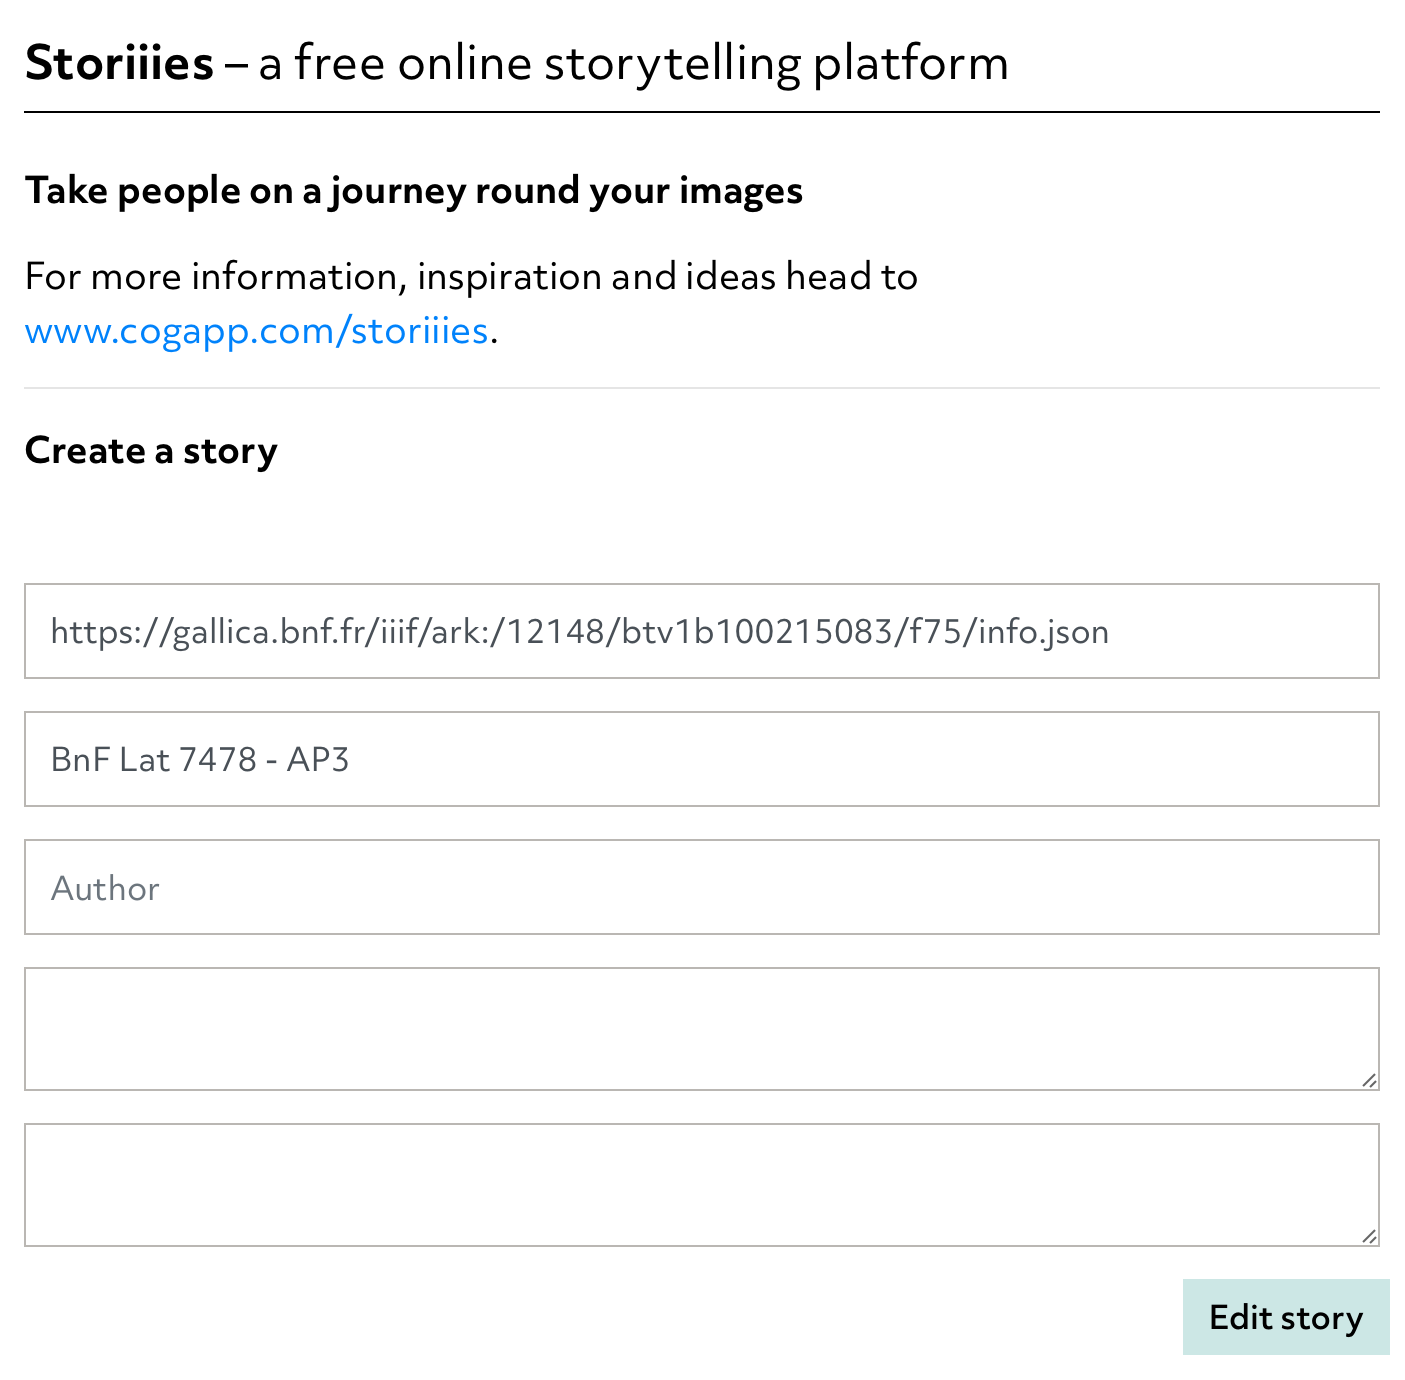
\includegraphics[scale=0.4, angle=0]{images/partie3/storiiies/storiiies-editor.png}
    \centering
    \end{figure}
	
	L'interface d'édition est minimale, ce qui rend sa prise en main très simple. Il suffit d'ajouter le lien du fichier \texttt{manifest.json}, récupéré sur le site d'une institution ou créé selon la méthode tout juste décrite. Il convient ensuite de préciser un titre à donner à la \textit{story} ainsi créée et d'indiquer qui en l'auteur. Enfin, le texte qui accompagnera l'image peut être inséré dans les cases prévues à cet effet. Une fois tout cela fait, cliquer sur \textit{Edit story} permet d'accéder à une nouvelle page par le biais de laquelle l'auteur peut visualiser la \textit{story} créée et obtenir le lien pour la réutiliser notamment dans un site web grâce à une balise \texttt{<iframe>}. 
	
	Storiiies Editor est donc un outil qu'il est aisé de prendre en main et qui permlet d'aboutir à un résultat tout à fait satisfaisant mais il présente néanmoins un inconvénient majeur : il permet de réaliser des \textit{stories} à partir d'un unique \textit{manifest}, or dans le cadre de cette exposition cela peut rapidement poser problème puisqu'au sein d'un même parcours il est question de plusieurs manuscrits. En effet, cela nécessiterait de créer un \textit{manifest} pour chaque parcours et ne permettrait pas de réutiliser ceux qui existent déjà. 
	
	\subsubsection{Omeka Classic - Exhibit Builder}
	Un autre outils compatible avec l'utilisation d'images \acrshort{iiif} est le \textit{plugin} Exhibit Builder d'Omeka Classic. C'est un outil qui permet lui aussi le développement en ligne d'exposition. Contrairement à Storiiies, ce \textit{plugin} permet de concevoir le site web dans son intégralité et pas seulement le contenu des différents parcours. Les \textit{exhibits} créés sont composés d'une ou plusieurs page(s) et la mise en page peut être personnalisée grâce à l'utilisation de différents blocs permettant d'insérer du texte ou des images.  
	
	Omeka est l'outil qui a été choisi par plusieurs institutions françaises pour le développement de leurs expositions en ligne, notamment dans le monde universitaire. Parmi elles, on peut citer \acrshort{psl}, l'\acrshort{inha}, la \acrshort{bis} ou encore l'\acrshort{ens}. Faire ce même choix serait donc cohérent avec les pratiques actuelles de la recherche française en sciences humaines. Malgré cela, ce n'est pas non plus l'outil qui a été retenu par l'équipe du projet notamment du fait de l'aspect plus statique que peuvent avoir les expositions ainsi réalisées par rapport à ce qu'il est possible d'obtenir en utilisant un outil pour le seul contenu des parcours et en développant intégralement le site web.
	
	\subsection{Exhibit}
	\subsubsection{Choix de cet outil}
    Exhibit est un outil qui utilise le protocole \acrshort{iiif} et dont le fonctionnement est très proche de celui de Storiiies Editor avec notamment la même possibilité d'intégrer les \textit{exhibits} à un site web. Néanmoins, une différence majeure est à noter : il est possible de créer un \textit{exhibit} à partir de plusieurs fichiers \texttt{manifest.json}. C'est donc en partie ce qui a justifié le choix de travailler avec cet outil. Une autre fonctionnalité intéressante est la possibilité de dupliquer un \textit{exhibit}, cela se révélera utile quand surviendra la création de versions longues et courtes de certains des parcours.
    
    Par ailleurs, quatre \textit{templates} sont disponibles pour créer un \textit{exhibit} : \textit{kiosk}, \textit{scroll}, \textit{slides} et \textit{quiz}. \textit{Kiosk} permet permet de déterminer un temps pour chaque \textit{slide} et le défilement est automatique une fois l'\textit{exhibit} lancé. Comme son nom le suggère, le \textit{template scroll} permet de parcourir l'\textit{exhibit} grâce au \textit{"scrollytelling}, c'est à dire que le visiteur navigue dans le parcours en faisant défiler les différentes \textit{slides} sur son écran. Le \textit{template slides} quant à lui permet de passer d'une \textit{slide} à l'autre en utilisant les flèches du clavier ou celles qui sont à disposition sur l'écran. Enfin, le \textit{template quiz} fonctionne de la même manière que le précédent mais il est possible d'ajouter des \textit{pinpoints} qui sont des marqueurs qui peuvent être placés sur des points précis de l'image que l'on souhaite signaler au visiteur. De plus, il est possible d'intégrer des questions. Or, l'une des idées évoquées lors de la préparation de cette exposition était d'intégrer des jeux pour rendre ludique la navigation. Ce \textit{template} apparaît donc comme une bonne solution pour y parvenir.
    
    \begin{figure}[h]
	\caption{Paramètres de création d'un \textit{exhibit}}
	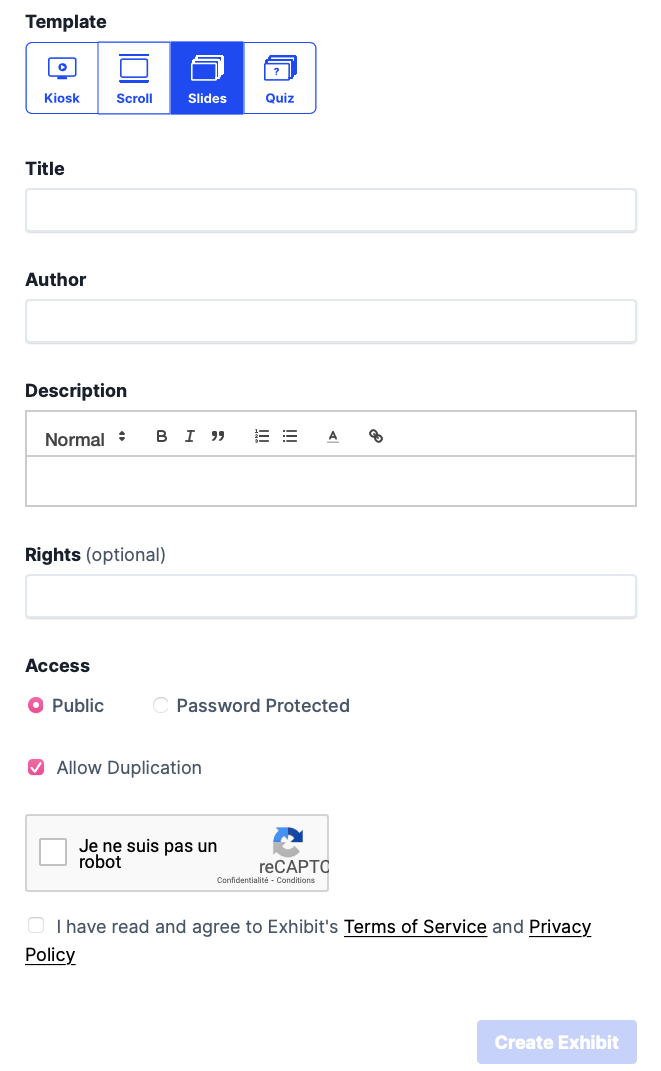
\includegraphics[scale=0.5, angle=0]{images/partie3/exhibit/exhibit-settings.png}
    \centering
    \end{figure}
    
    Avant de commencer à ajouter du contenu, il faut donc définir certains paramètres, en premier lieu le \textit{template}. Dans le cadre de l'exposition \textit{Medieval skies under(book)cover}, seul le \textit{template quiz} est utilisé. Il est ensuite nécessaire de définir un titre pour l'\textit{exhibit}, c'est le nom du parcours correspondant qui peut donc être utilisé. Un auteur et une description font aussi partie des éléments requis avant de pouvoir créer un \textit{exhibit}. 
    
	\subsubsection{Création de contenu grâce à cet outil} 
	Une fois l'\textit{exhibit} créé, du contenu peut y être intégré. Par contenu, on entend ici les \textit{attention points} du parcours que l'on souhaite ajouter. Comme précédemment précisé, il est possible d'ajouter plusieurs \textit{manifests}. Toutefois, il faut être vigilant à bien sélectionner le bon \textit{manifest} lorsque l'on veut ajouter des \textit{attention points} afin de pouvoir associer le texte rédigé en amont au folio correspondant. 
	
	\begin{figure}[h]
	\caption{Interface d'ajout d'un \textit{manifest}}
	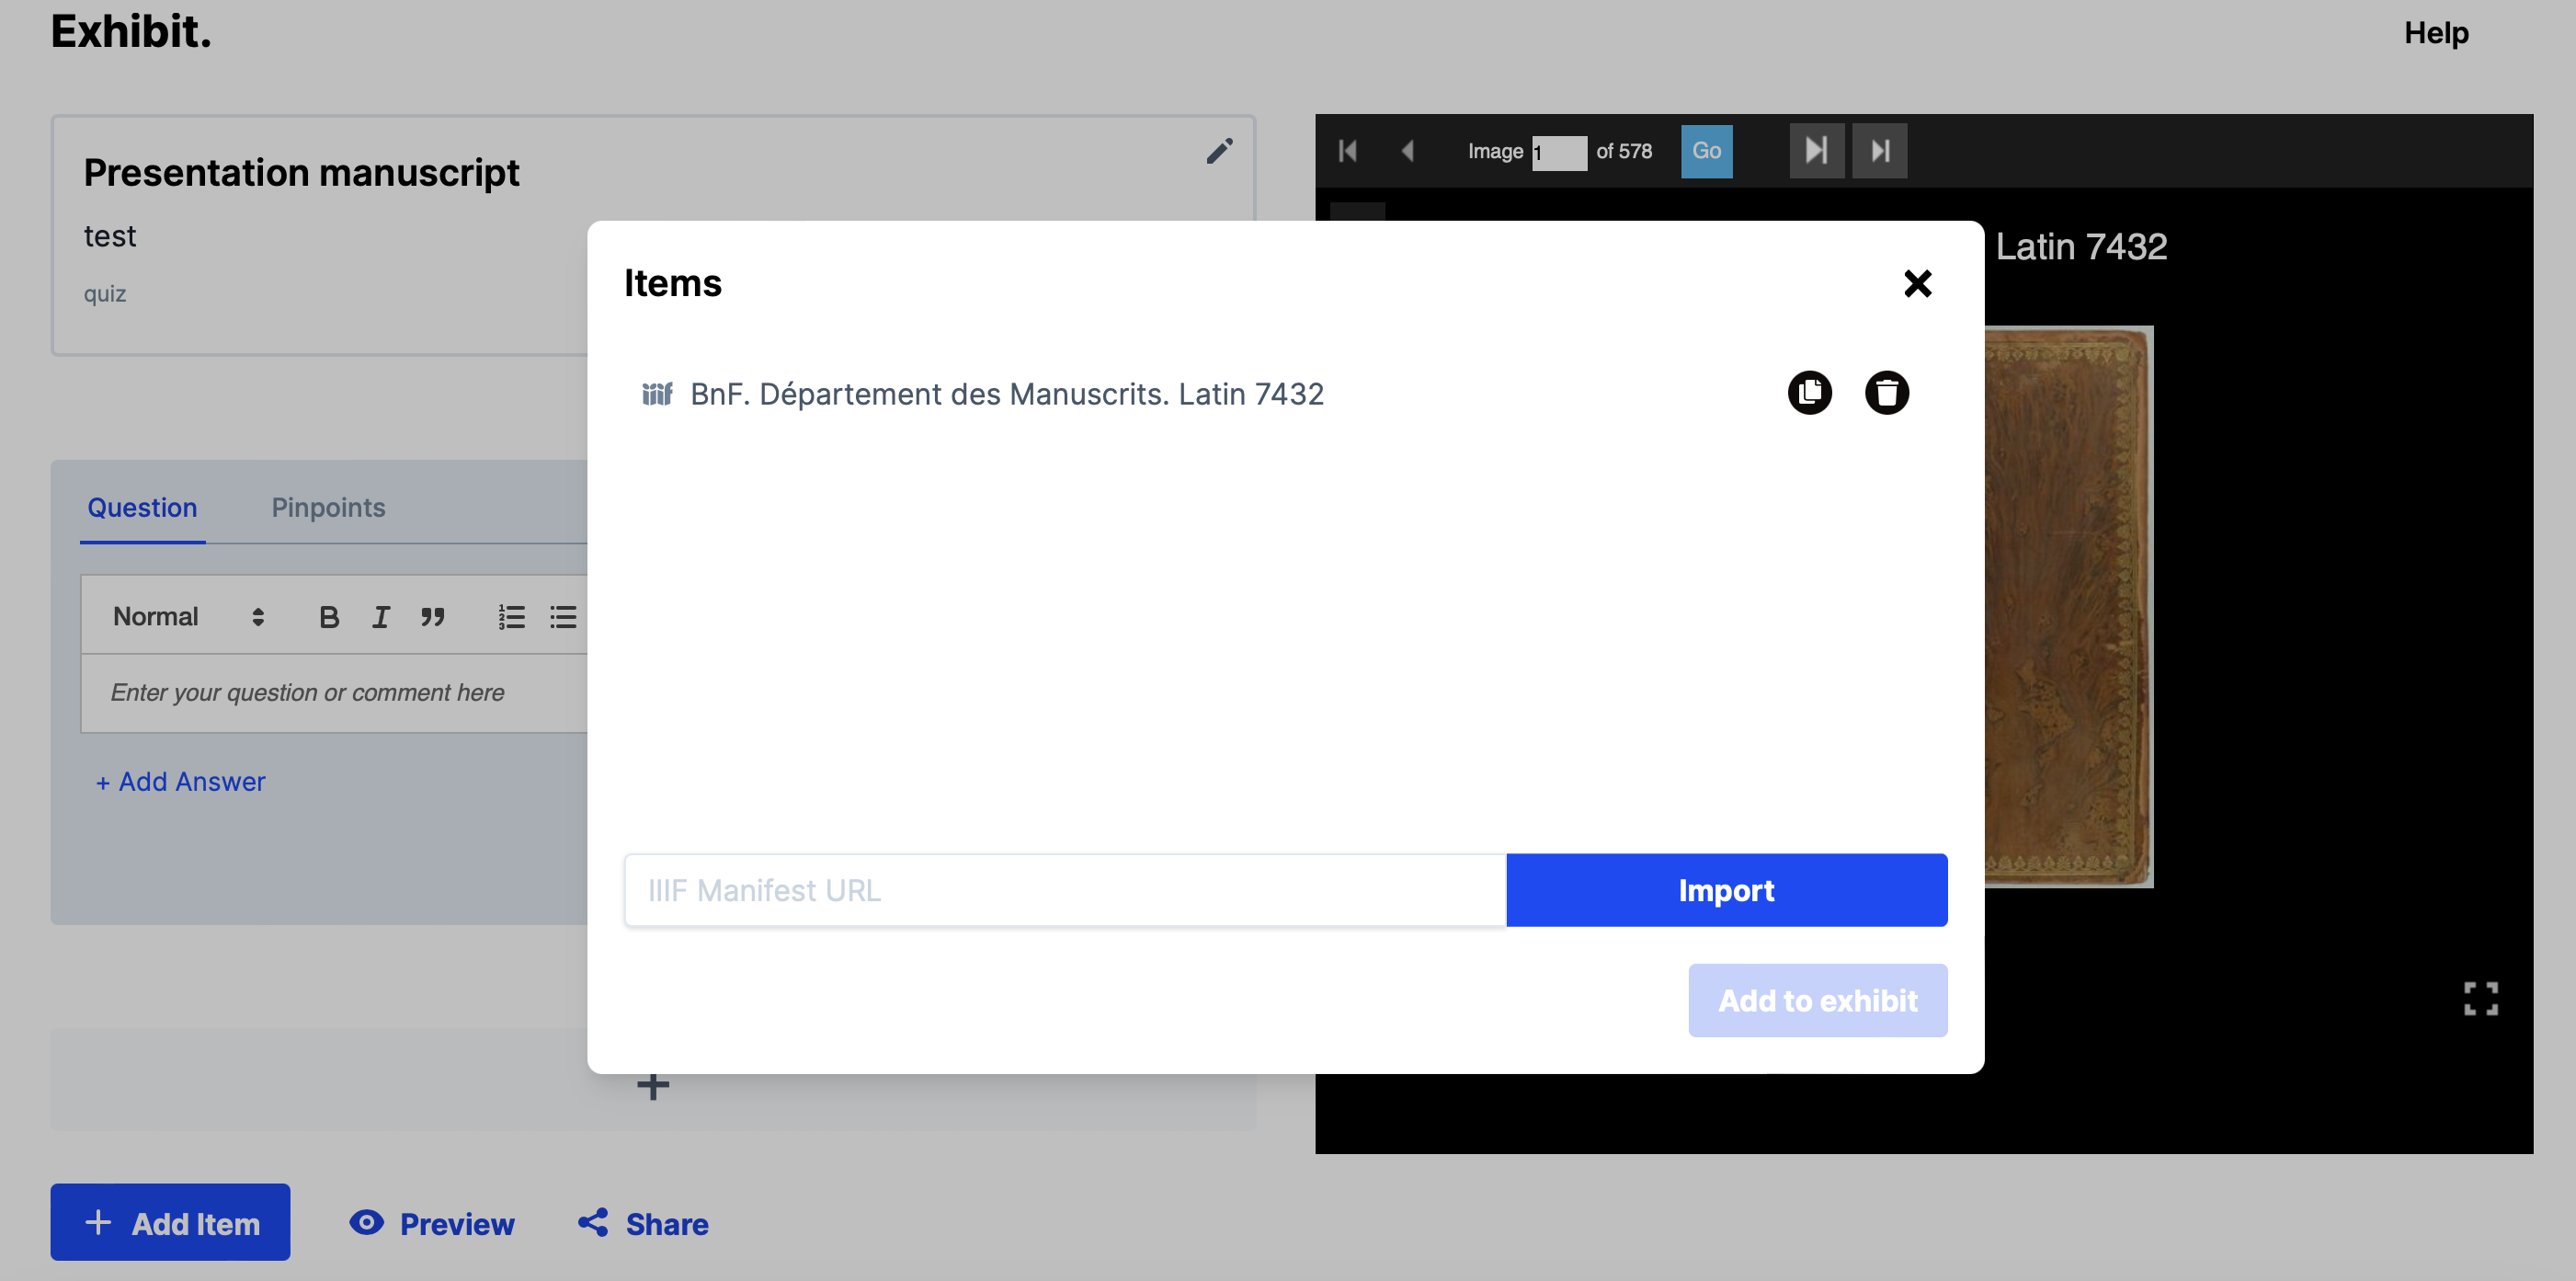
\includegraphics[scale=0.2, angle=0]{images/partie3/exhibit/exhibit-manifest.png}
    \centering
    \end{figure}
    
    
    \begin{figure}[h]
	\caption{Interface d'ajout de \textit{captions}}
	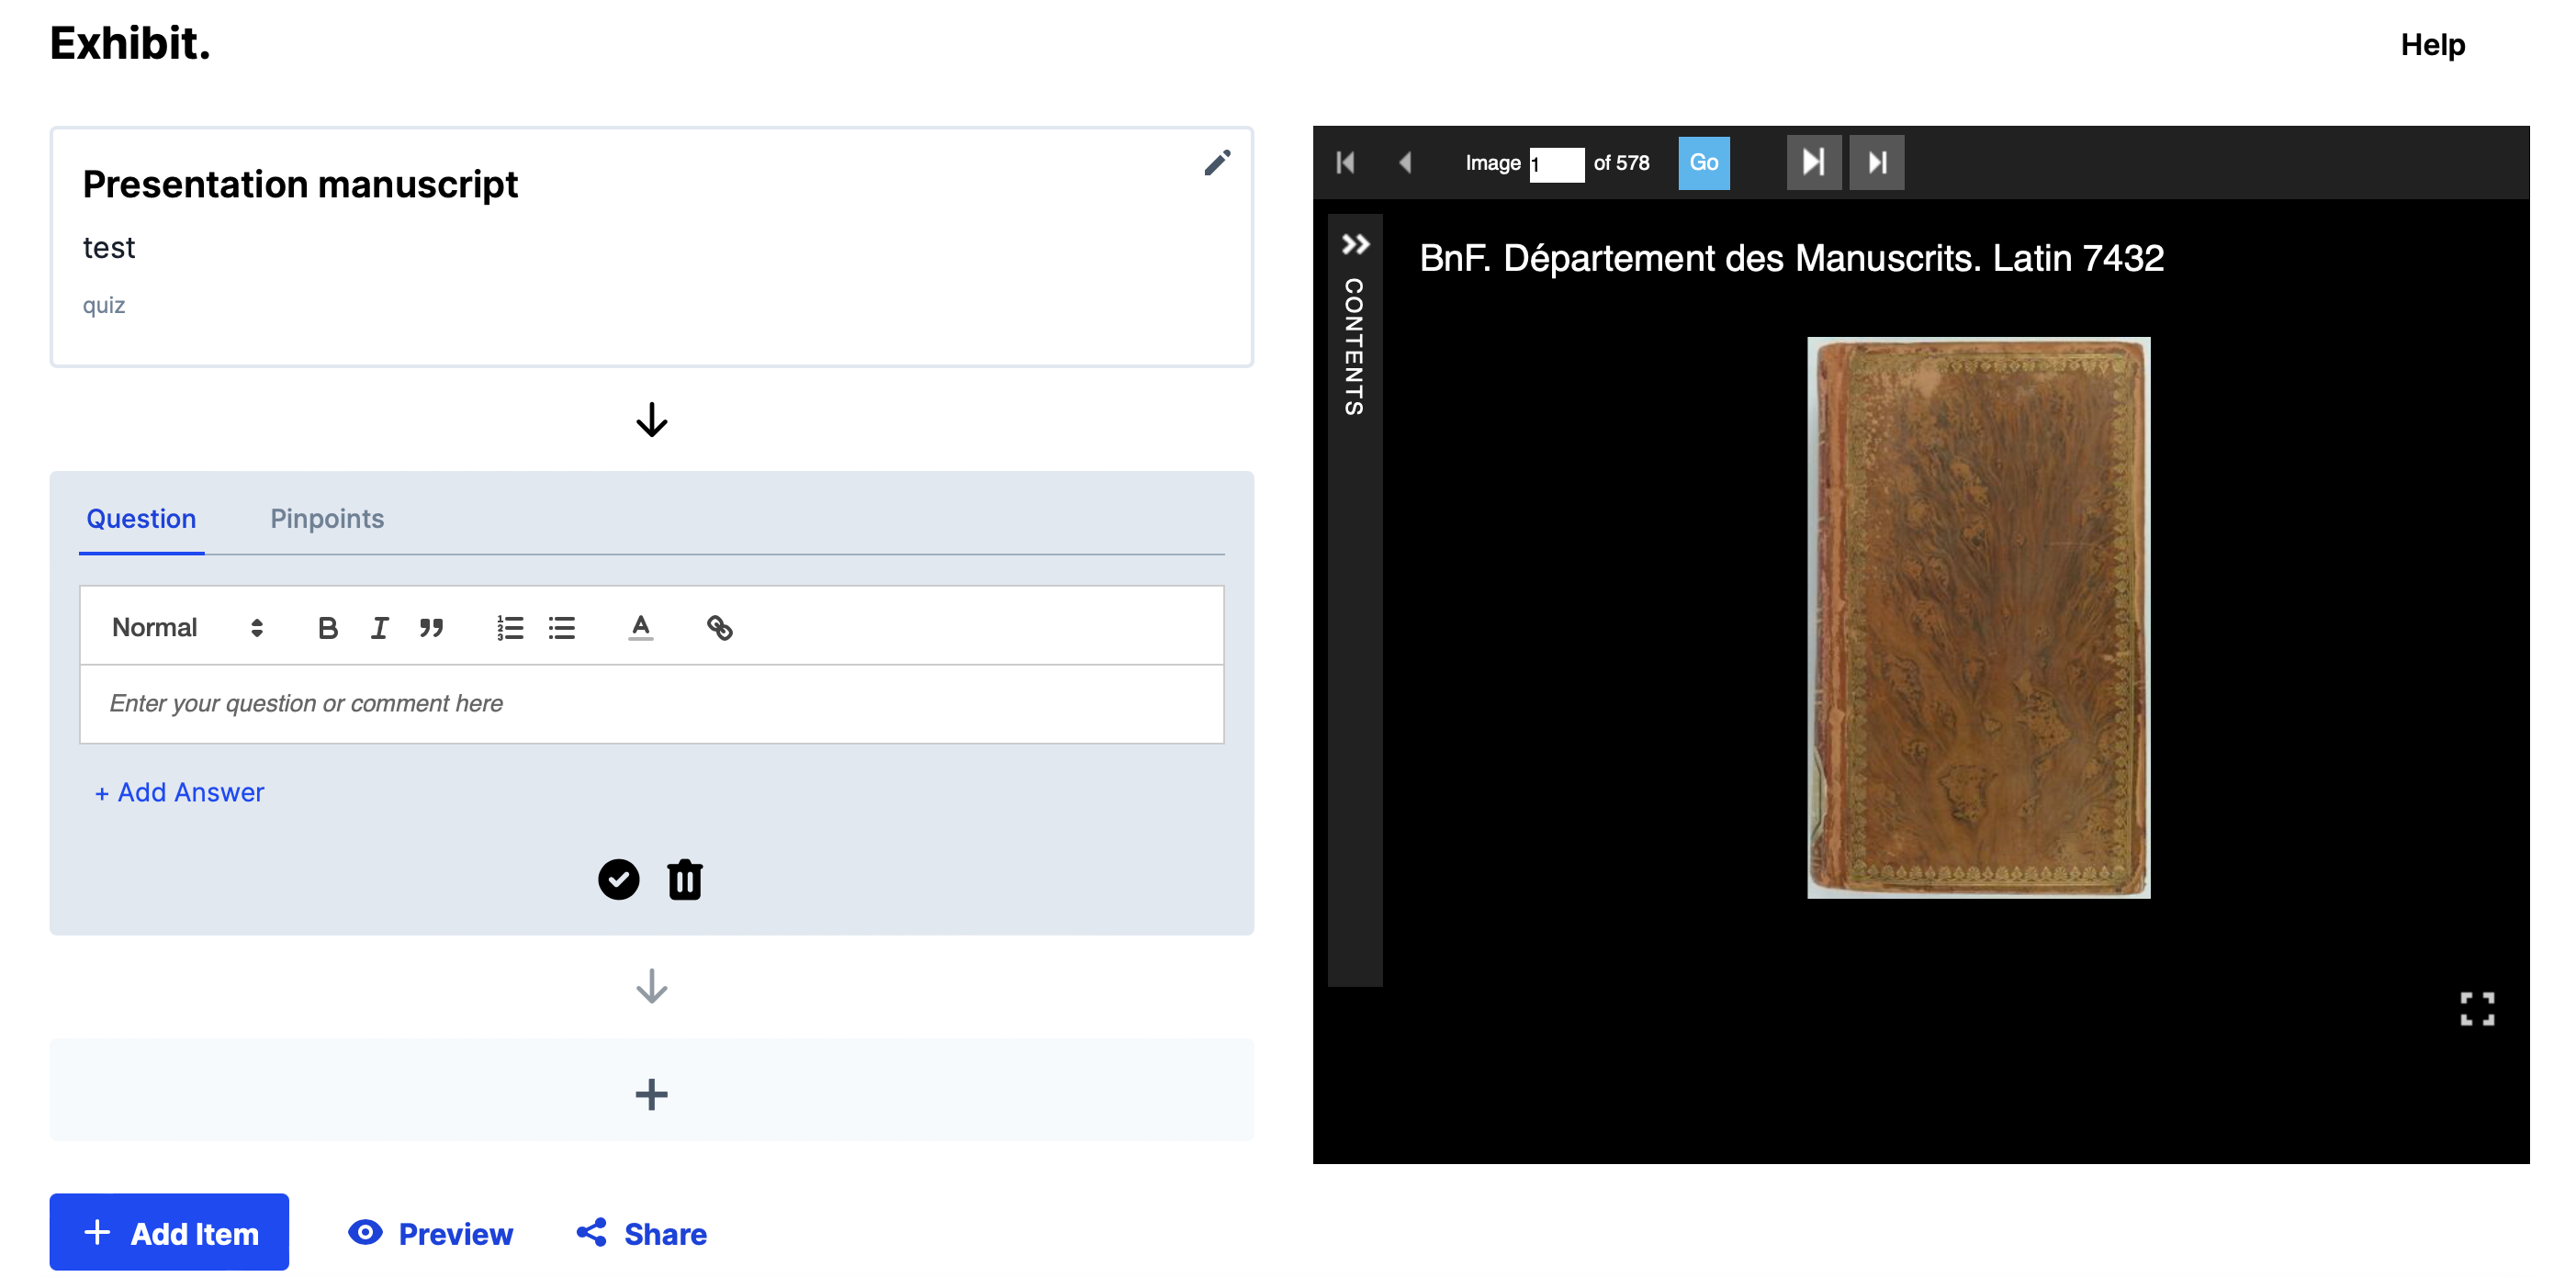
\includegraphics[scale=0.3, angle=0]{images/partie3/exhibit/exhbit-captions.png}
    \centering
    \end{figure}
    
    Sur l'interface d'Exhibit, les descriptions associées aux images sont appelées des \textit{captions}. C'est donc là que les \textit{attention points} sont recopiés et qu'ils vont pouvoir être mis en forme. En effet, il est possible de mettre des éléments en gras ou en italique pour souligner leur importance aux yeux du lecteur. C'est également dans cette interface que l'auteur pourra choisir le folio à associer et choisir, s'il le souhaite, de zoomer sur une partie précise de celui. Comme indiqué, pour plus de précisions encore, l'utilisation de \textit{pinpoints} est possible et c'est dans cette même interface que cela se fait. 
    
    Pour satisfaire les besoins de la scénographie, les \textit{attention points} ne sont pas toujours utilisés tels qu'ils ont été produits par les chercheurs. En effet, s'ils sont trop longs notamment ils peuvent être découpés en plusieurs \textit{captions}, chacune associée à un zoom qui est donc plus précis du folio liée à l'\textit{attention point} \footnote{Pour plus de précision concernant les transformations des \textit{attention points} lors de leur intégration aux \textit{exhibits}, voir annexe \ref{Tutoriel}, à la page \pageref{Tutoriel}.}. La création des \textit{exhibits} pour chacun des parcours thématiques et manuscrits et la formalisation de recommandations pour les phases de relecture par les chercheurs ont occupé une grande partie de mon stage à l'Observatoire. Néanmoins, les \textit{attention points} n'ont, pour la plupart, été intégrés que dans leur version initiale et il reviendra aux chercheurs de les retravailler pour mettre en lumière les éléments qui méritent de l'être. Par ailleurs, quand des parcours raccourcis seront ajoutés, les \textit{exhibits} devront de nouveau faire l'objet d'une relecture pour ajouter si nécessaire des liens permettant aux visiteurs de naviguer d'un \textit{shortcut} à un autre. 
    
	\subsubsection{Ajout de fonctionnalité}
	Évoquée au début de cette partie, la communauté \acrshort{iiif} est véritablement active et participative. Ainsi, prendre contact avec l'un des développeurs d'Exhibit, Edward Silverton, s'est fait sans encombre. L'objectif était alors de discuter de la possibilité d'ajouter une fonctionnalité à Exhibit : le \textit{deeplinking} ou la création de liens spécifiques à chaque \textit{slide} d'un \textit{exhibit}. En effet, jusqu'alors le lien renvoyait systématiquement au début. La perspective de ces liens plus précis représente un atout important pour le futur de l'exposition et la création de versions courtes pour certains parcours. Cette fonctionnalité a pu être implémentée rapidement, bien avant la fin du stage, ce qui a permis de la tester et de valider ainsi la proposition faite par Edward Silverton. Chaque \textit{slide} a donc désormais un identifiant qui lui est propre, à la fin de son url \acrshort{url}. 
	
	Cet ajout est déjà utilisé dans l'exposition pour le glossaire. En effet, dans celui-ci sont référencées toutes les mentions des différentes figures historiques au sein de l'exposition et pour chacune il a donc été possible d'indiquer le folio exact d'un manuscrit en renvoyant le visiteur avec précision vers la \textit{slide} concernée.

	
	\chapter{Élaboration de l’application web}
	Le présent chapitre est consacré au développement effectif de l'application web destinée à la visite de l'exposition \textit{Medieval skies under(book)cover}. Il y sera alors principalement question du code et de la manière dont il a été pensé et élaboré. 
	
	\section{Architecture de l’application flask}
	
    \subsection{Pages HTML}
    \subsubsection{\textit{Homepage}}
    \begin{figure}[h]
	\caption{Page d'accueil du site \textit{Medieval skies under(book)cover}}
	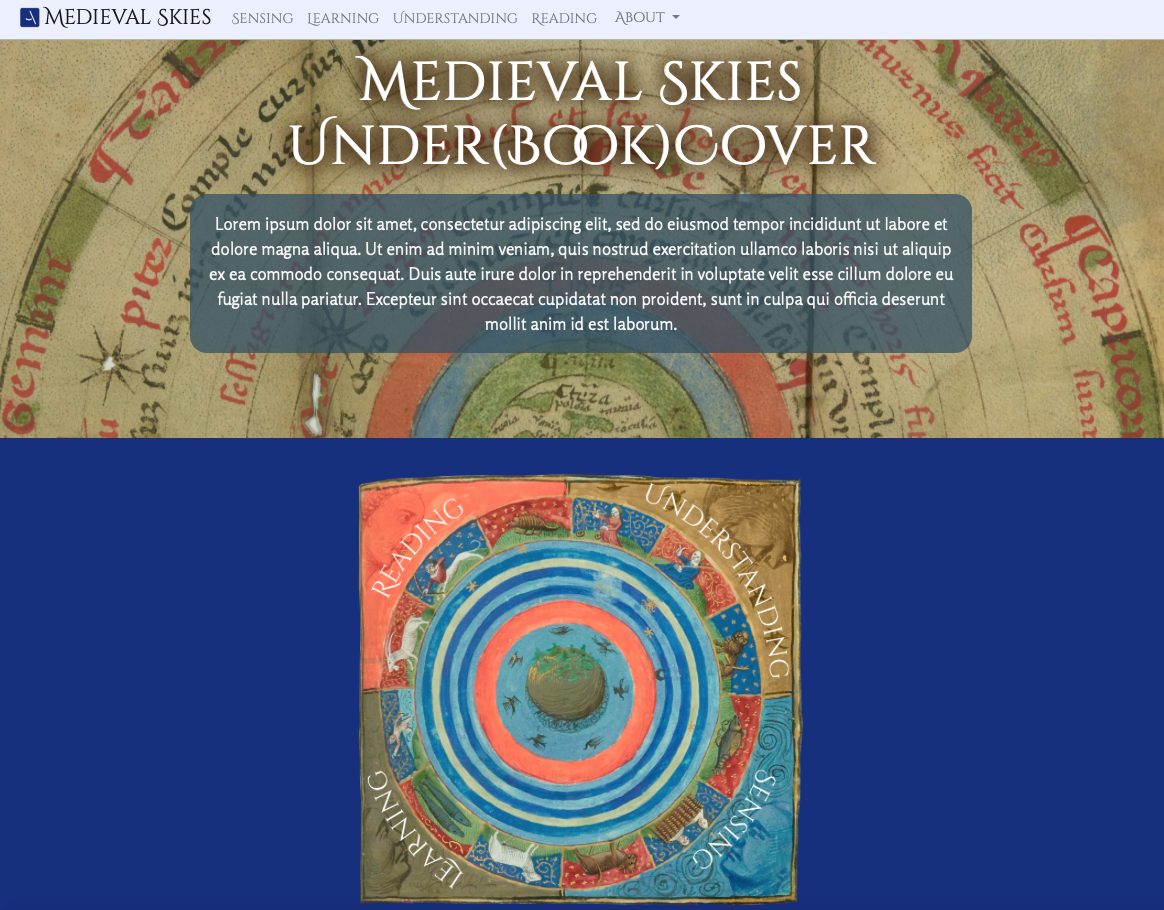
\includegraphics[scale=0.3, angle=0]{images/partie3/website/expo-homepage.png}
    \centering
    \end{figure}
    
    C'est ainsi que débute la visite de l'exposition. Dès le départ, le visiteur a donc face à lui des morceaux de manuscrits, l'une et l'autre des images choisies sont issus du manuscrit de présentation de Conrad Heingarter \footnote{Il s'agit du manuscrit Paris, BnF | Lat. 7432.}. Une description générale de l'exposition accompagnera bientôt le titre dans la partie haute de la page. La partie centrale est quant à elle interactive : les utilisateurs ont la possibilité de cliquer sur l'une des quatre parties\footnote{\textit{Sensing} renvoie aux parcours patrimoniaux, \textit{Learning} à ceux liés à l'histoire de l'astronomie alphonsine, \textit{Understanding} à ceux qui expliquent les notions scientifiques et \textit{Reading} à ceux qui mettent en lumière les manuscrits un à un.} de l'image, où sont représentés des vents, pour accéder au thème indiqué sur la partie choisie. Ces quatre thèmes sont également accessibles en cliquant sur le nom souhaité dans la barre de navigation. Grâce à cette même \textit{navbar}, la page d'accueil est accessible depuis toutes les pages du site web en cliquant sur le titre dans une version raccourcie, \textit{Medieval skies}. Cela respecte les attentes notées dans le document de spécification. Que le visiteur choisisse la barre de navigation ou la miniature interactive, une très brève description des thèmes est affichée au survol avec la souris, permettant de le guider dans son choix. Plus bas, la possibilité est offerte aux visiteurs de se rendre directement sur la page d'un des parcours désignés comme étant à voir absolument. Enfin, le pied de page, commun à l'ensemble du site web, permet de connaître les principaux partenaires et d'accéder à leurs propres sites web par un clic sur le logo. 
    
    \subsubsection{\textit{Themes}}
    Après avoir choisi un thème à visiter, l'utilisateur découvre l'une de ces quatre pages \footnote{Elles sont accessibles : \href{https://alfa-exhibition.herokuapp.com/heritage}{\textit{Sensing}}, \href{https://alfa-exhibition.herokuapp.com/historical}{\textit{Learning}}, \href{https://alfa-exhibition.herokuapp.com/scientific}{\textit{Understanding}} et \href{https://alfa-exhibition.herokuapp.com/manuscripts}{\textit{Reading}}.}, chacune construite selon le même principe. 
    
    \begin{figure}[!h]
    \centering
    \begin{subfigure}[h]{0.4\textwidth}
        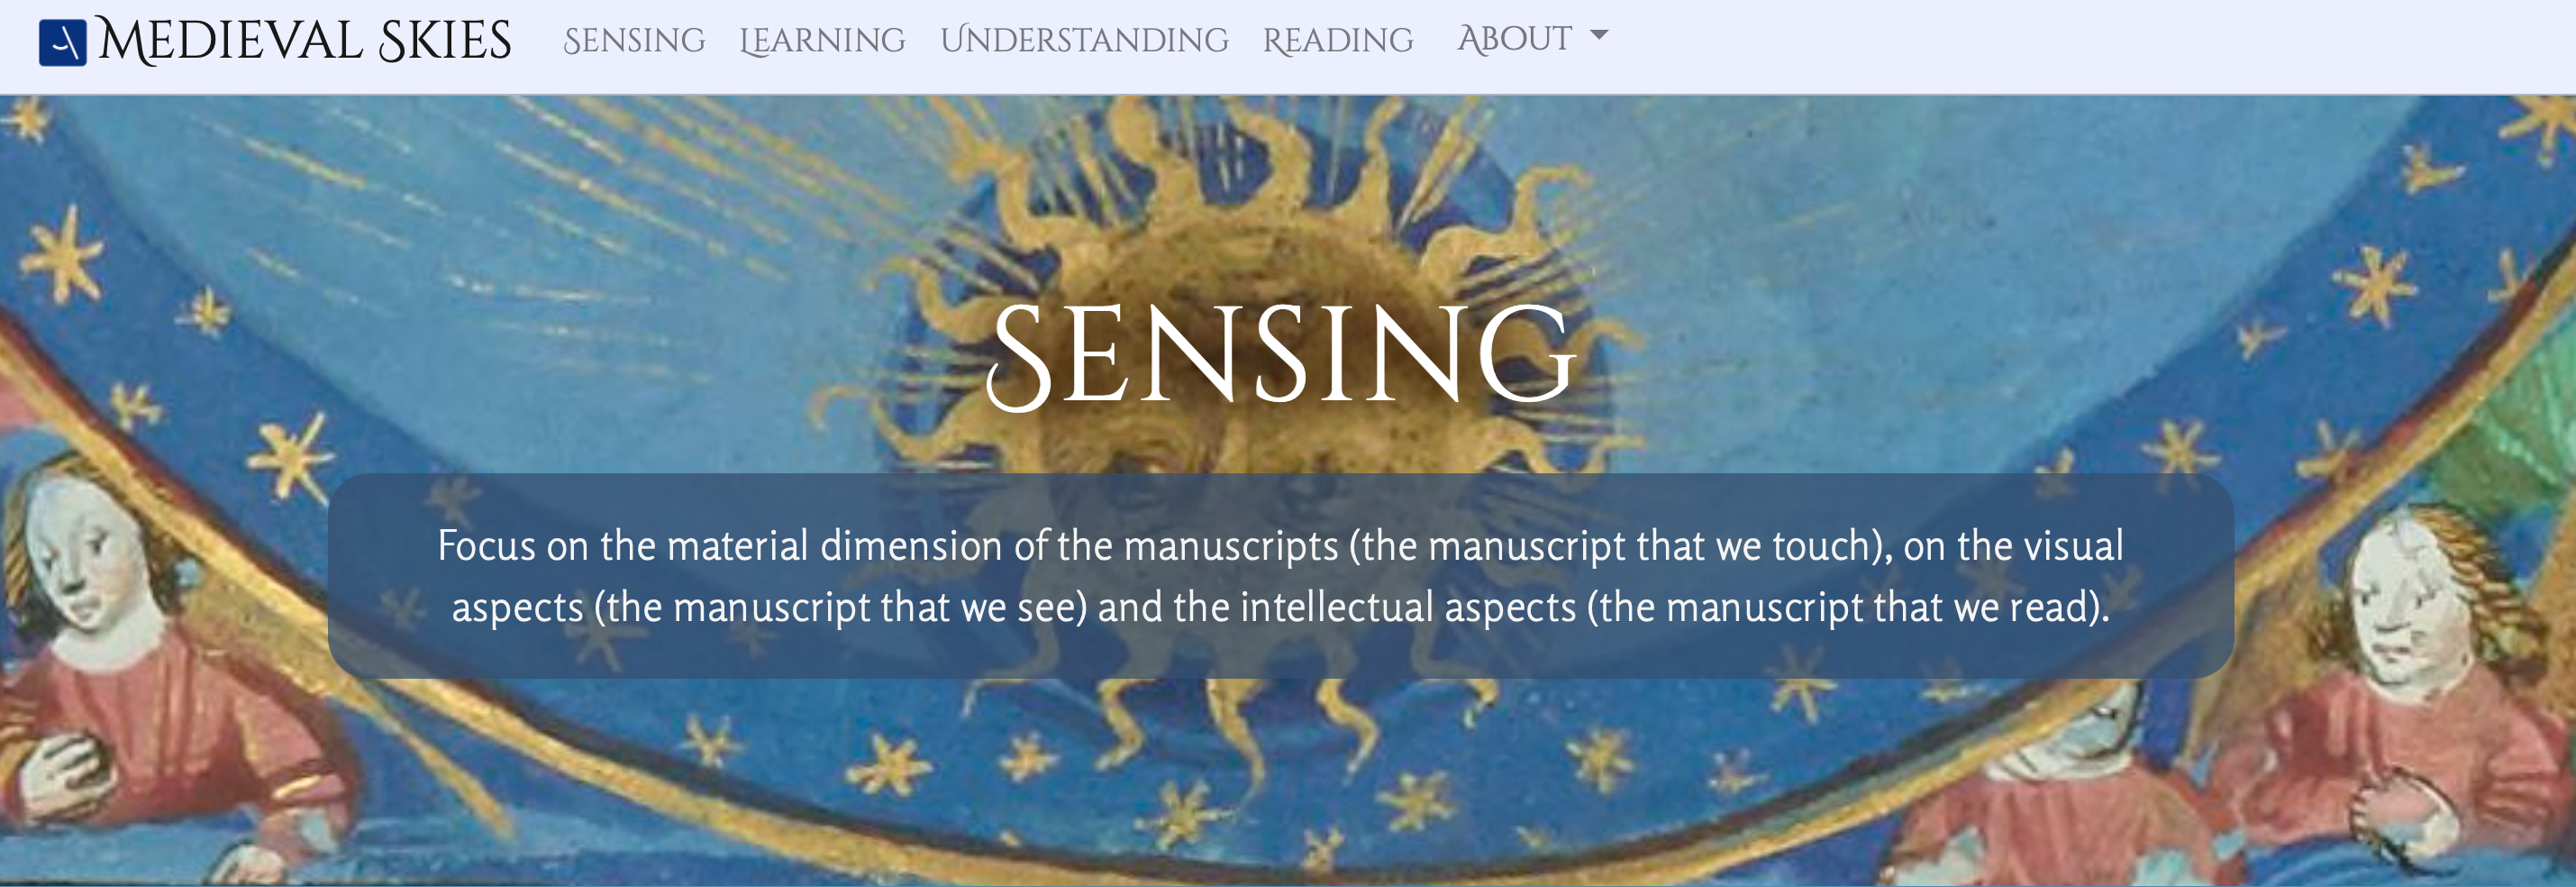
\includegraphics[width=\textwidth]{images/partie3/website/expo-sensing.png}
    \end{subfigure}
    \begin{subfigure}[h]{0.4\textwidth}
        \includegraphics[width=\textwidth]{images/partie3/website/expo-learning.png}
    \end{subfigure}
    \begin{subfigure}[h]{0.4\textwidth}
        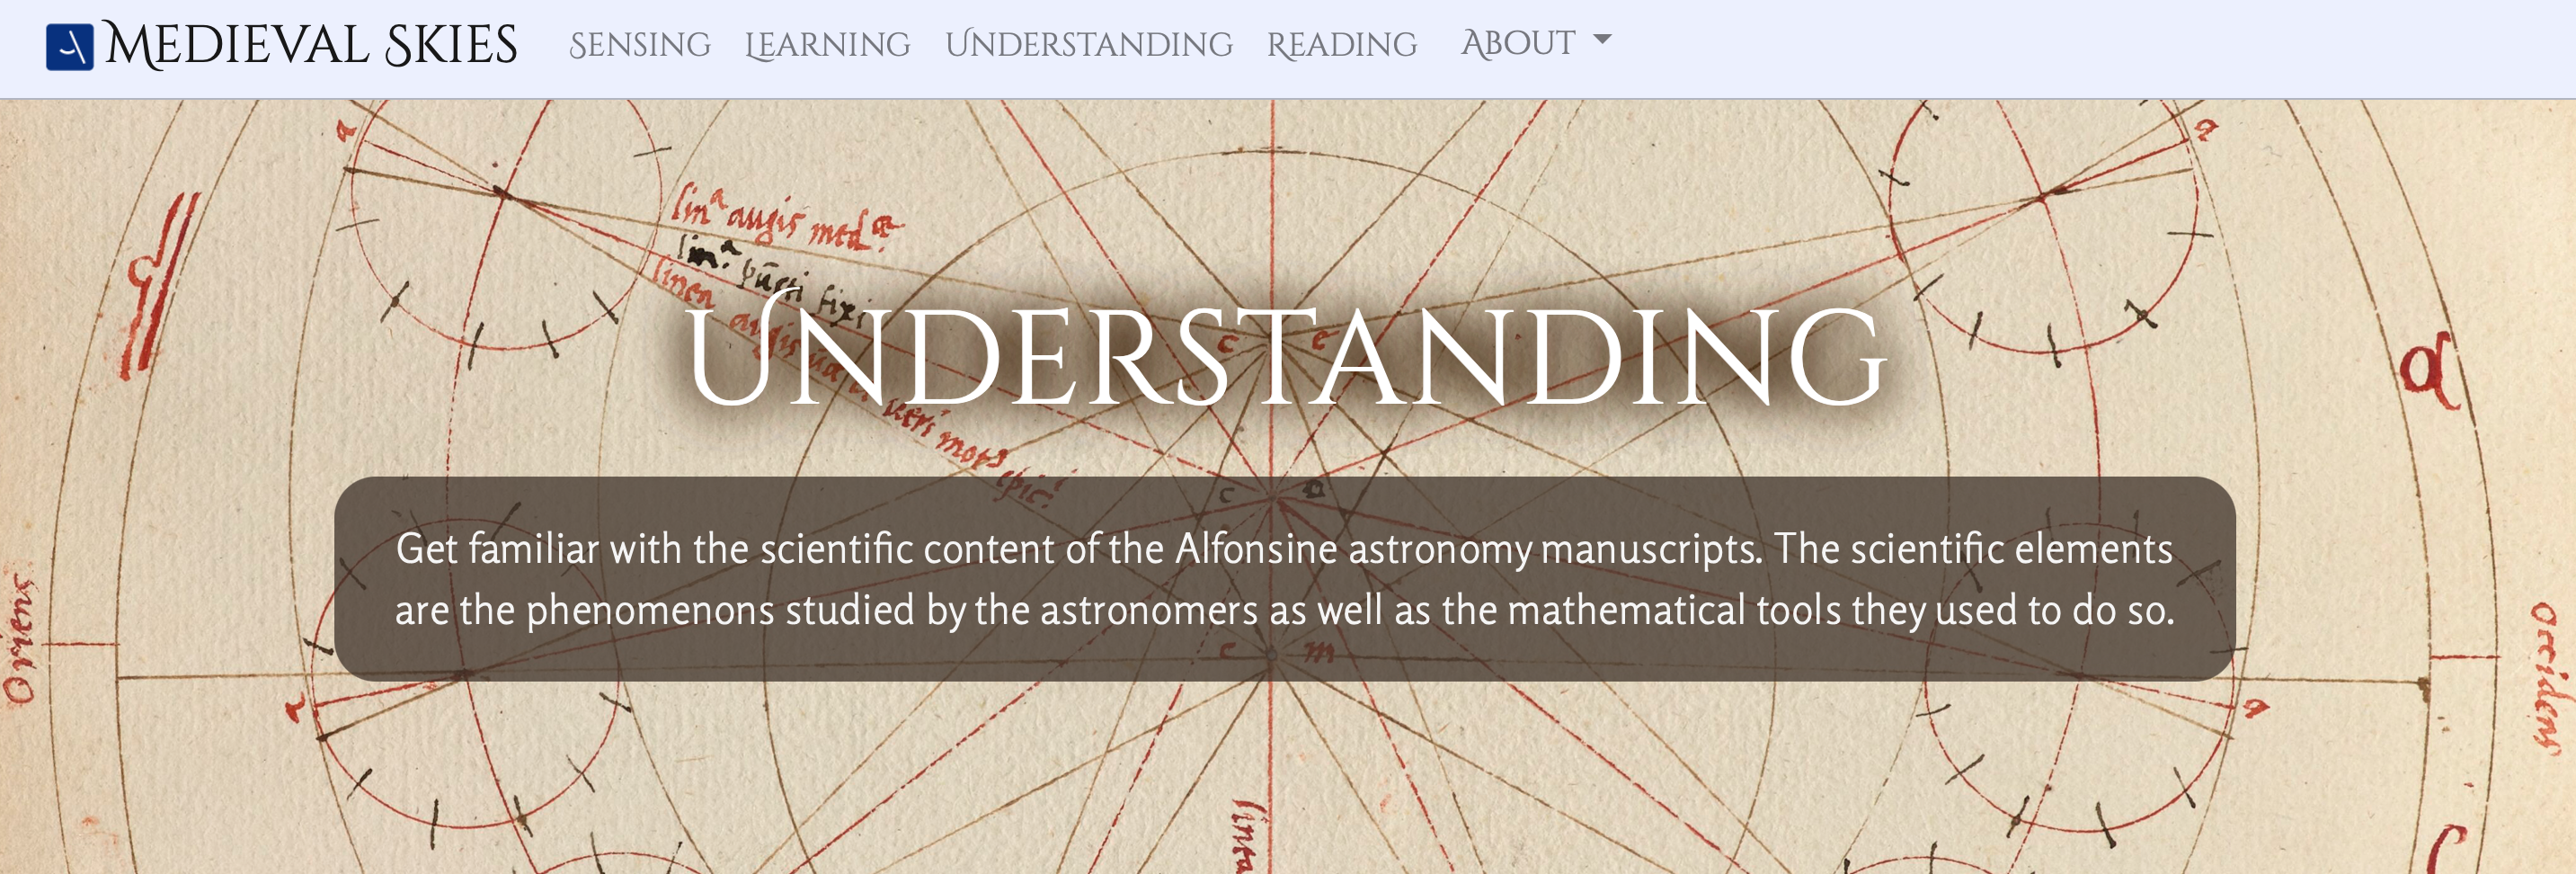
\includegraphics[width=\textwidth]{images/partie3/website/expo-understanding.png}
    \end{subfigure}
    \begin{subfigure}[h]{0.4\textwidth}
        \includegraphics[width=\textwidth]{images/partie3/website/expo-reading.png}
    \end{subfigure}
    \caption{Pages \textit{Sensing}, \textit{Learning}, \textit{Understanding} et \textit{Reading} du site \textit{Medieval skies under(book)cover}}
    \end{figure}

    Les captures d'écran présentées ici correspondent à la partie supérieure de chacune de ces pages. On peut remarquer que la \textit{navbar} est toujours présente. Sous le titre des thèmes, une description plus longue du contenu est proposée afin d'aiguiller les visiteurs. Les images choisies proviennent à chaque fois d'un manuscrit exposé dans au moins un des parcours du thème choisi. 
    
    Plus bas sur chacune de ces pages, le visiteur a le choix parmi les différents parcours qui composent le thème où il se trouve.
    
    \begin{figure}[h]
	\caption{Page \textit{Reading} du site \textit{Medieval skies under(book)cover}}
	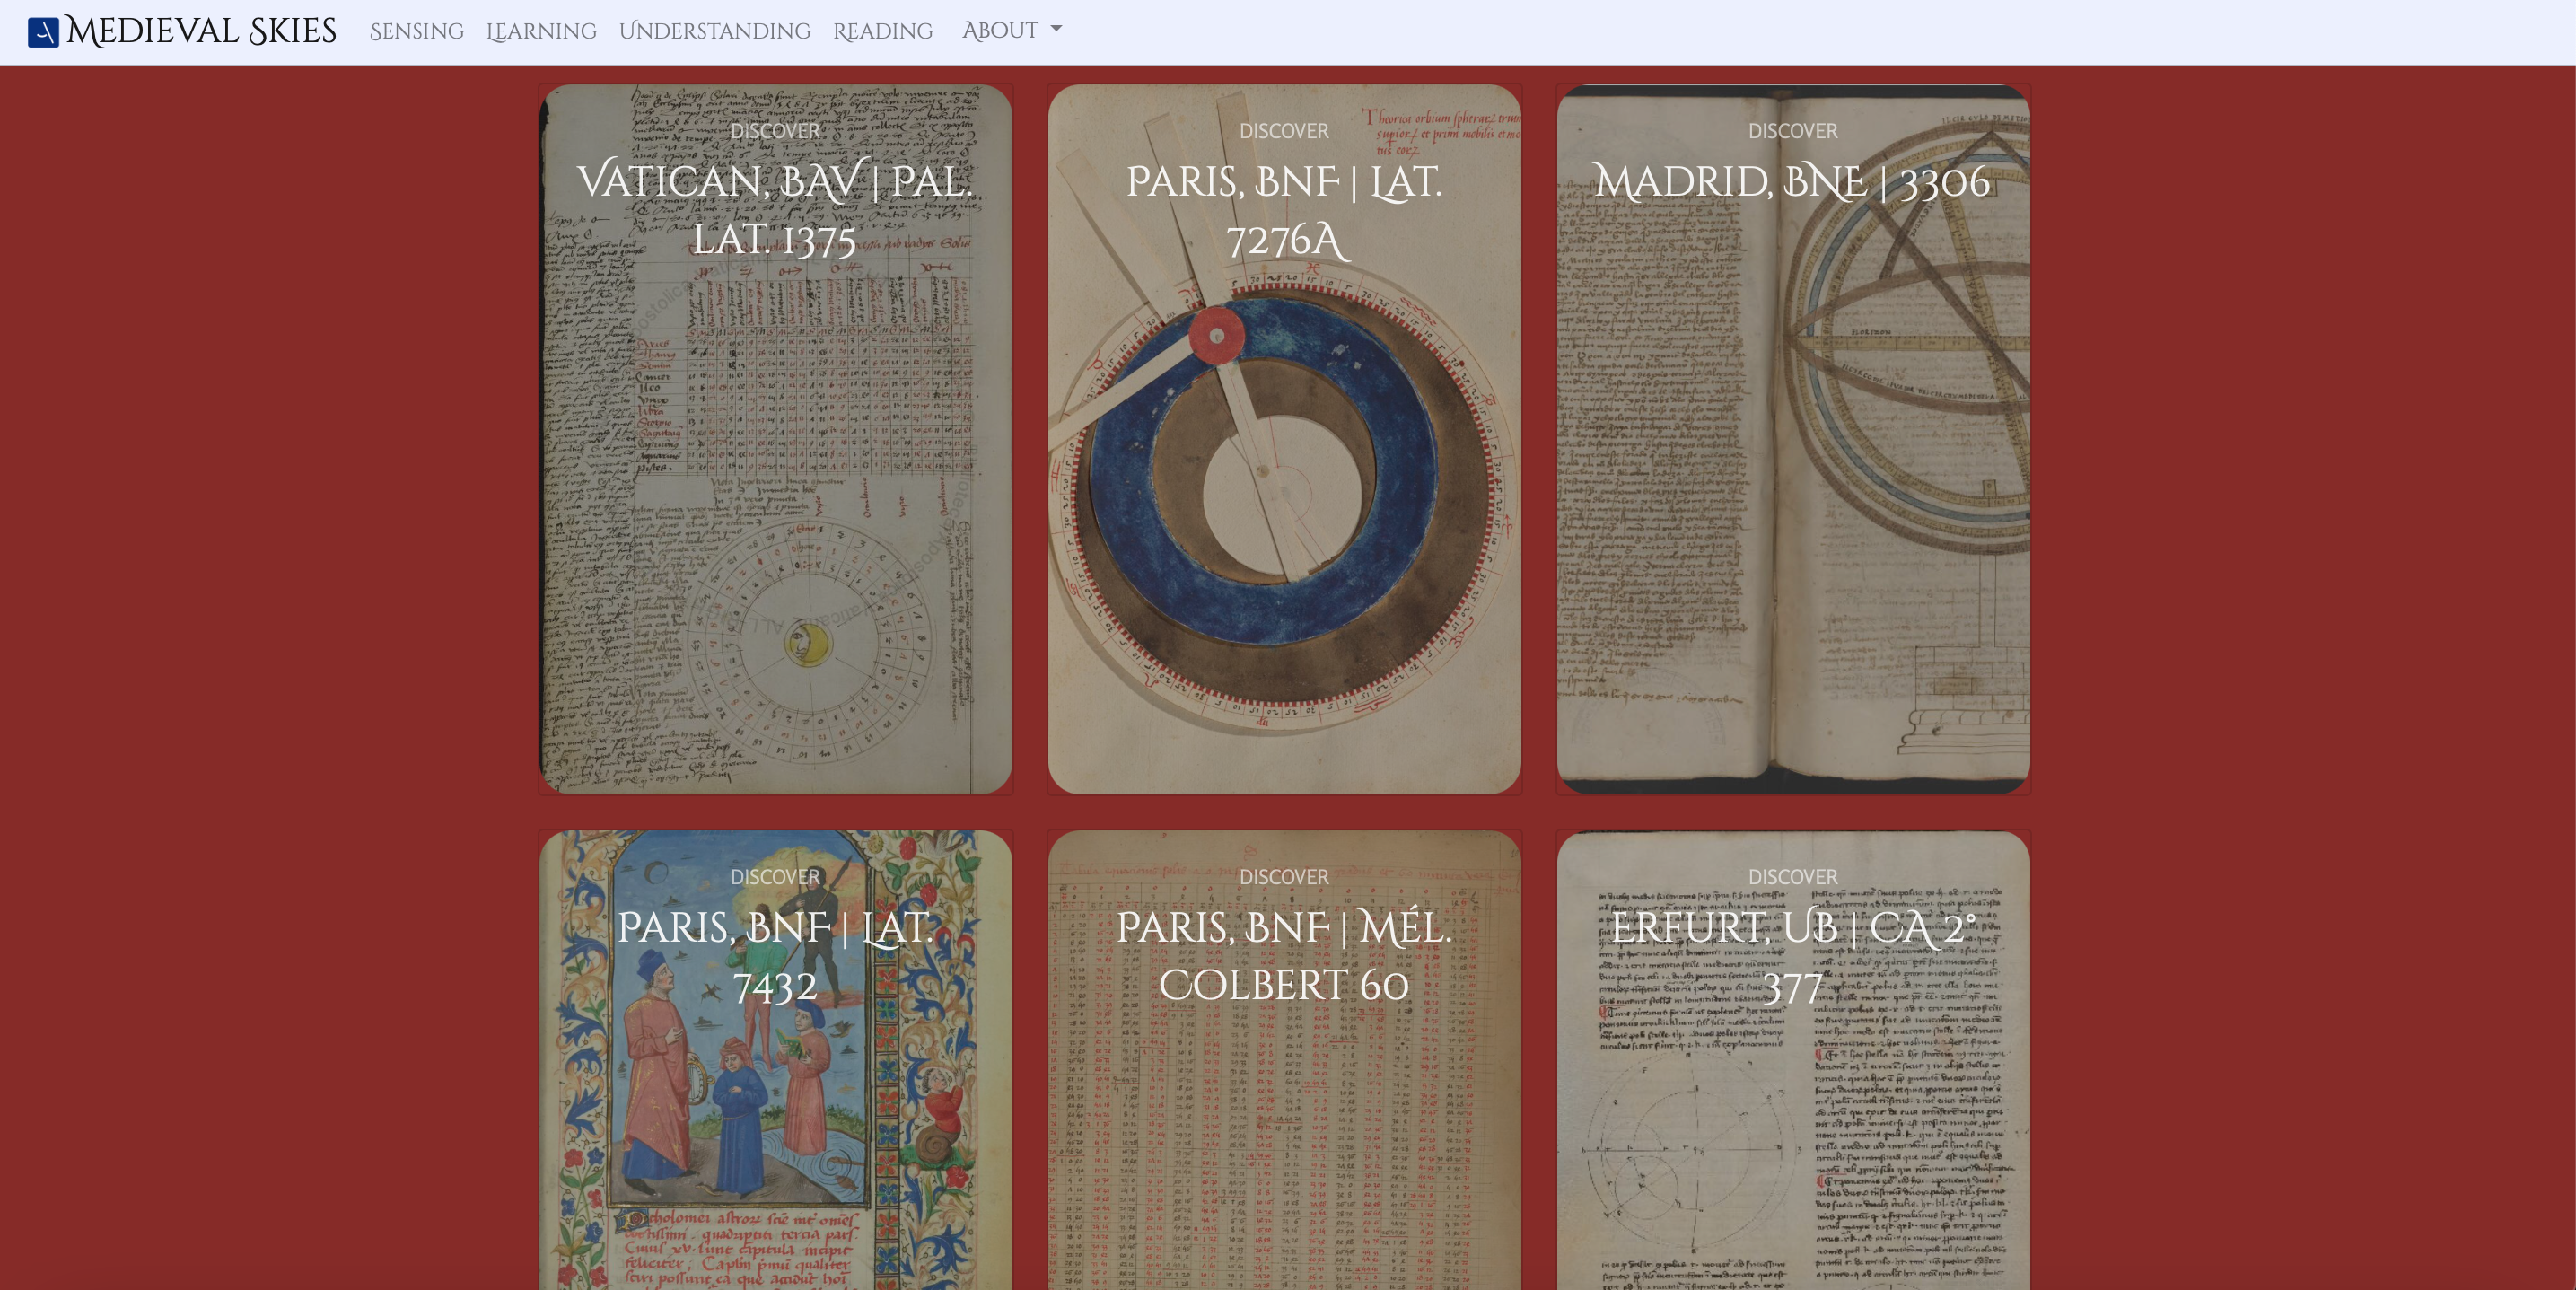
\includegraphics[scale=0.3, angle=0]{images/partie3/website/expo-reading-cards.png}
    \centering
    \end{figure}
    
    Seul est ici pris l'exemple du thème \textit{Reading} mais l'organisation est presque identique sur chacune des quatre pages : la seule différence étant le nombre de parcours, et donc de cartes cliquables, disponibles.
    
    Enfin, en bas de chacune de ces pages, le visiteur a à sa disposition un carrousel qui lui permet d'accéder aux trois autres thèmes depuis celui où il se trouve.  Prenons l'exemple de la page dédiée aux aspects patrimoniaux :
    
    \begin{figure}[h]
	\caption{Page \textit{Sensing} du site \textit{Medieval skies under(book)cover}}
	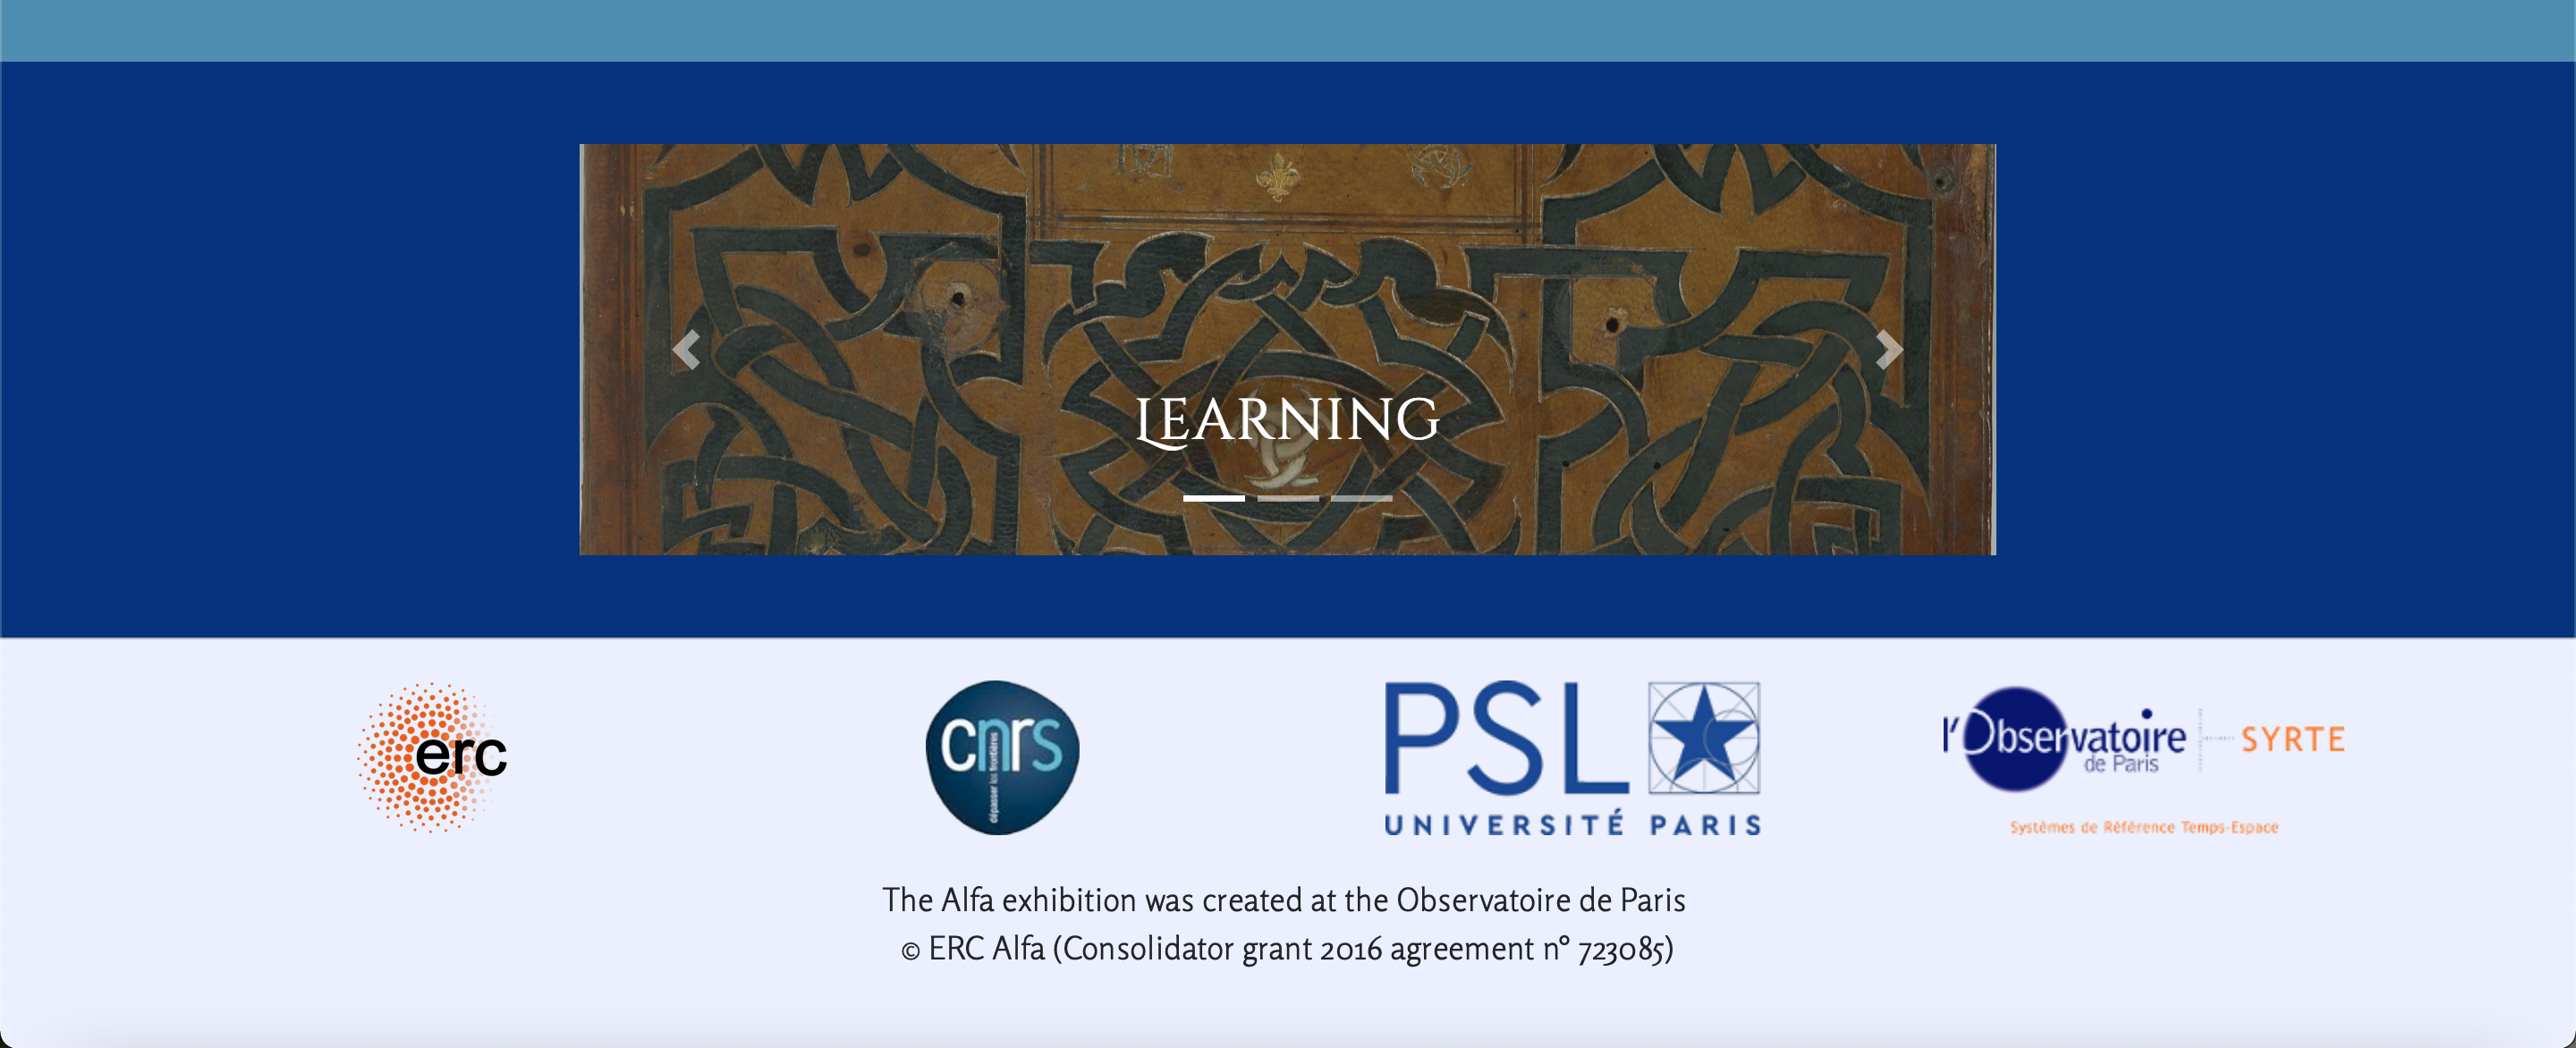
\includegraphics[scale=0.3, angle=0]{images/partie3/website/expo-sensing-carrousel.png}
    \centering
    \end{figure}
    
    On peut remarquer que l'image utilisée, ici pour le thème \textit{Learning} est la même qu'au début de la page de ce thème : c'est un autre moyen de guider les utilisateurs, en maintenant un cadre cohérent où ils peuvent se repérer aisément. 
    
    \subsubsection{\textit{Paths}}
    Pour accéder au parcours de son choix, le visiteur est appelé à cliquer sur la carte qui correspond à celui-ci. Là encore, tous les parcours se présentent de la même manière donc un unique exemple sera pris pour illustrer ce type de page.
    
    \begin{figure}[h]
	\caption{Page \textit{Exceptional manuscript} du site \textit{Medieval skies under(book)cover}}
	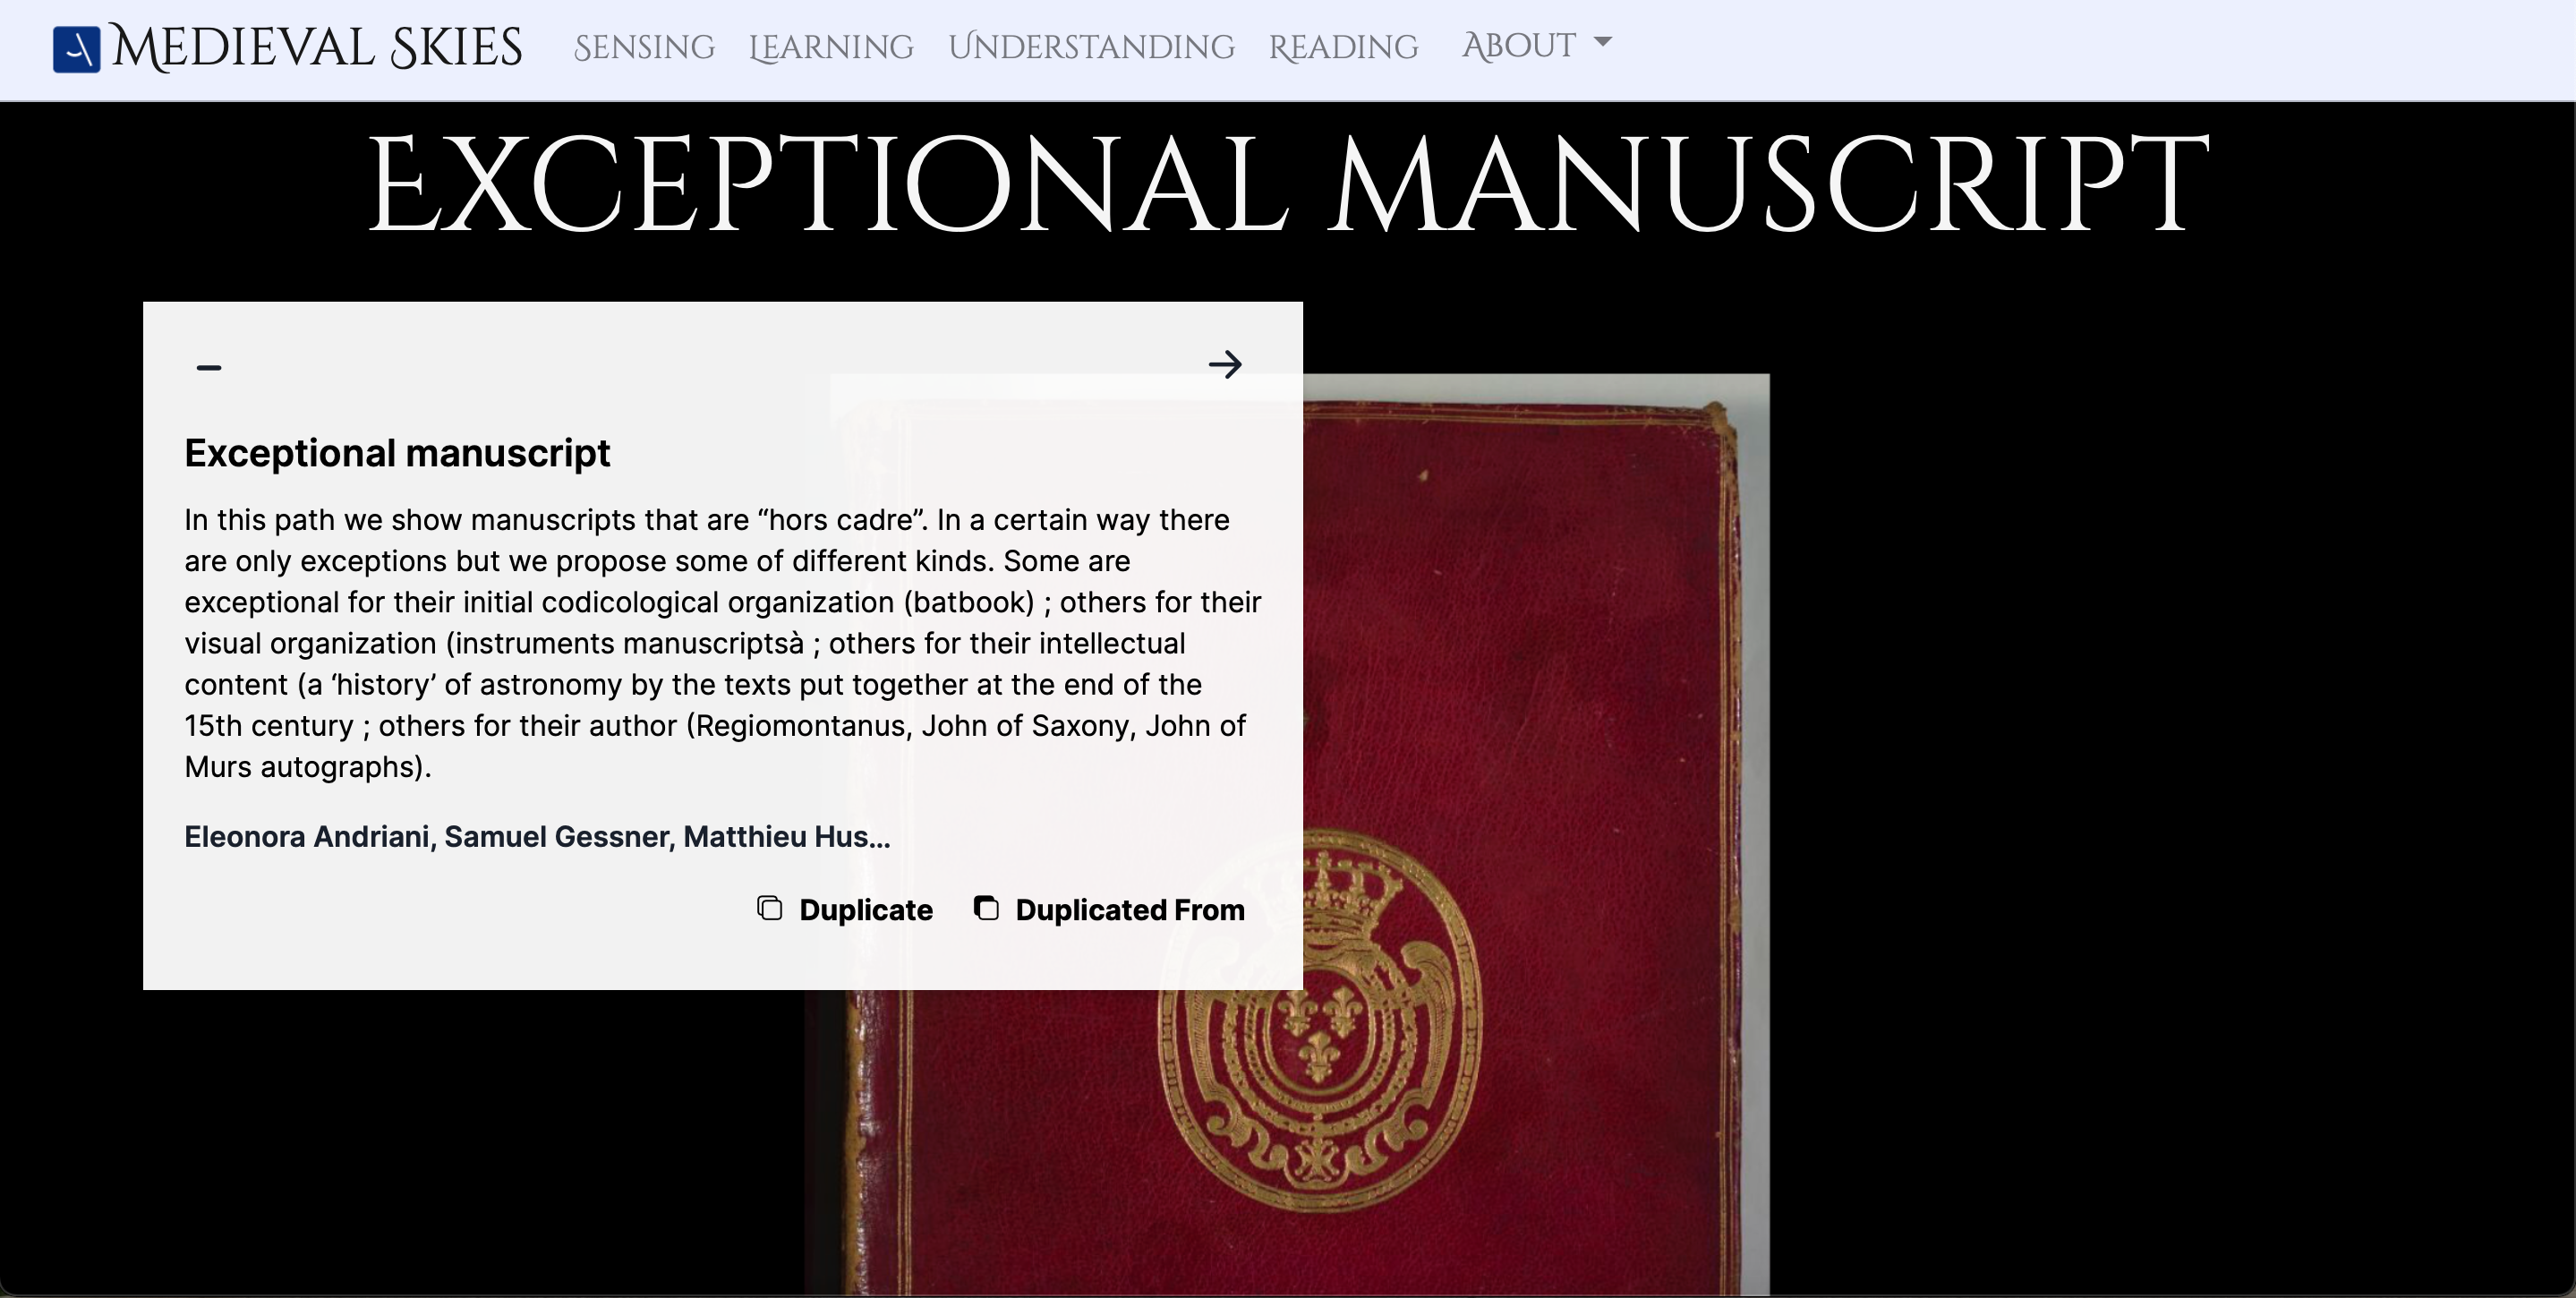
\includegraphics[scale=0.3, angle=0]{images/partie3/website/expo-paths-exceptional.png}
    \centering
    \end{figure}
    
    Outre la \textit{navbar} qui est toujours présente. Le visiteur accède ici à l'\textit{exhibit} créé pour ce parcours selon la méthode évoquée au précédent chapitre. Il peut ainsi découvrir les \textit{attention points} définis par les chercheurs. Une fois ce parcours terminé, il peut accéder aux autres parcours du même thème par le biais d'un carrousel en bas de page, de la même manière que ce qui a été montré pour les pages relatives aux quatre grands thèmes.
    
    \subsubsection{\textit{About}}
    Un élément de la \textit{navbar} n'a pas encore été évoqué : \textit{About}. C'est un menu déroulant qui permet d'accéder à trois autres pages qui ne contiennent pas de contenu directement inclus dans l'exposition. Ces pages sont les suivantes : \textit{About this project}, \textit{Glossary} et \textit{Bibliography} \footnote{Elles sont également accessibles : \href{https://alfa-exhibition.herokuapp.com/about}{\textit{About this project}}, \href{https://alfa-exhibition.herokuapp.com/glossary}{\textit{Glossary}} et \href{https://alfa-exhibition.herokuapp.com/bibliography}{\textit{Bibliography}}}. Ces pages ne sont pas encore finalisées : leur contenu doit être rédigé par l'équipe scientifique mais la structure est, elle, déjà en place. 
    
    Pour la page \textit{About this project}, l'idée est d'avoir une première section donnant aux visiteurs des précisions sur le projet \acrshort{alfa} au delà de l'exposition puis d'avoir un \textit{listing} des membres de l'équipe avant de terminer par quelques mots sur les institutions qui conservent les manuscrits utilisés dans cette exposition. 
    
    La page \textit{Bibliography} est la plus incomplète. Comme son nom le suggère, y seront renseignés des éléments bibliographiques qui permettront aux divers visiteurs d'accéder à des ressources complémentaires, plus précises et externes à l'exposition. Une seule référence est à ce jour visible dans le but de faire un test. Cela fait partie des éléments qui seront à compléter par l'équipe scientifique mais là encore, l'architecture de la page est prévue.
    
    Enfin, la page \textit{Glossary} qui, bien qu'incomplète, est la plus avancée des trois. C'est une sorte de répertoire des figures historiques : les liens des \textit{attention points} de l'exposition qui font mention de ces différents personnages y sont reportés, de même que ceux des notices Wikipedia et Biblissima, quand ces ressources existent. Les biographies qui viendront compléter ces références devront, quant à elle, être rédigées.
    
    \begin{figure}[!h]
    \centering
    \begin{subfigure}[h]{0.5\textwidth}
        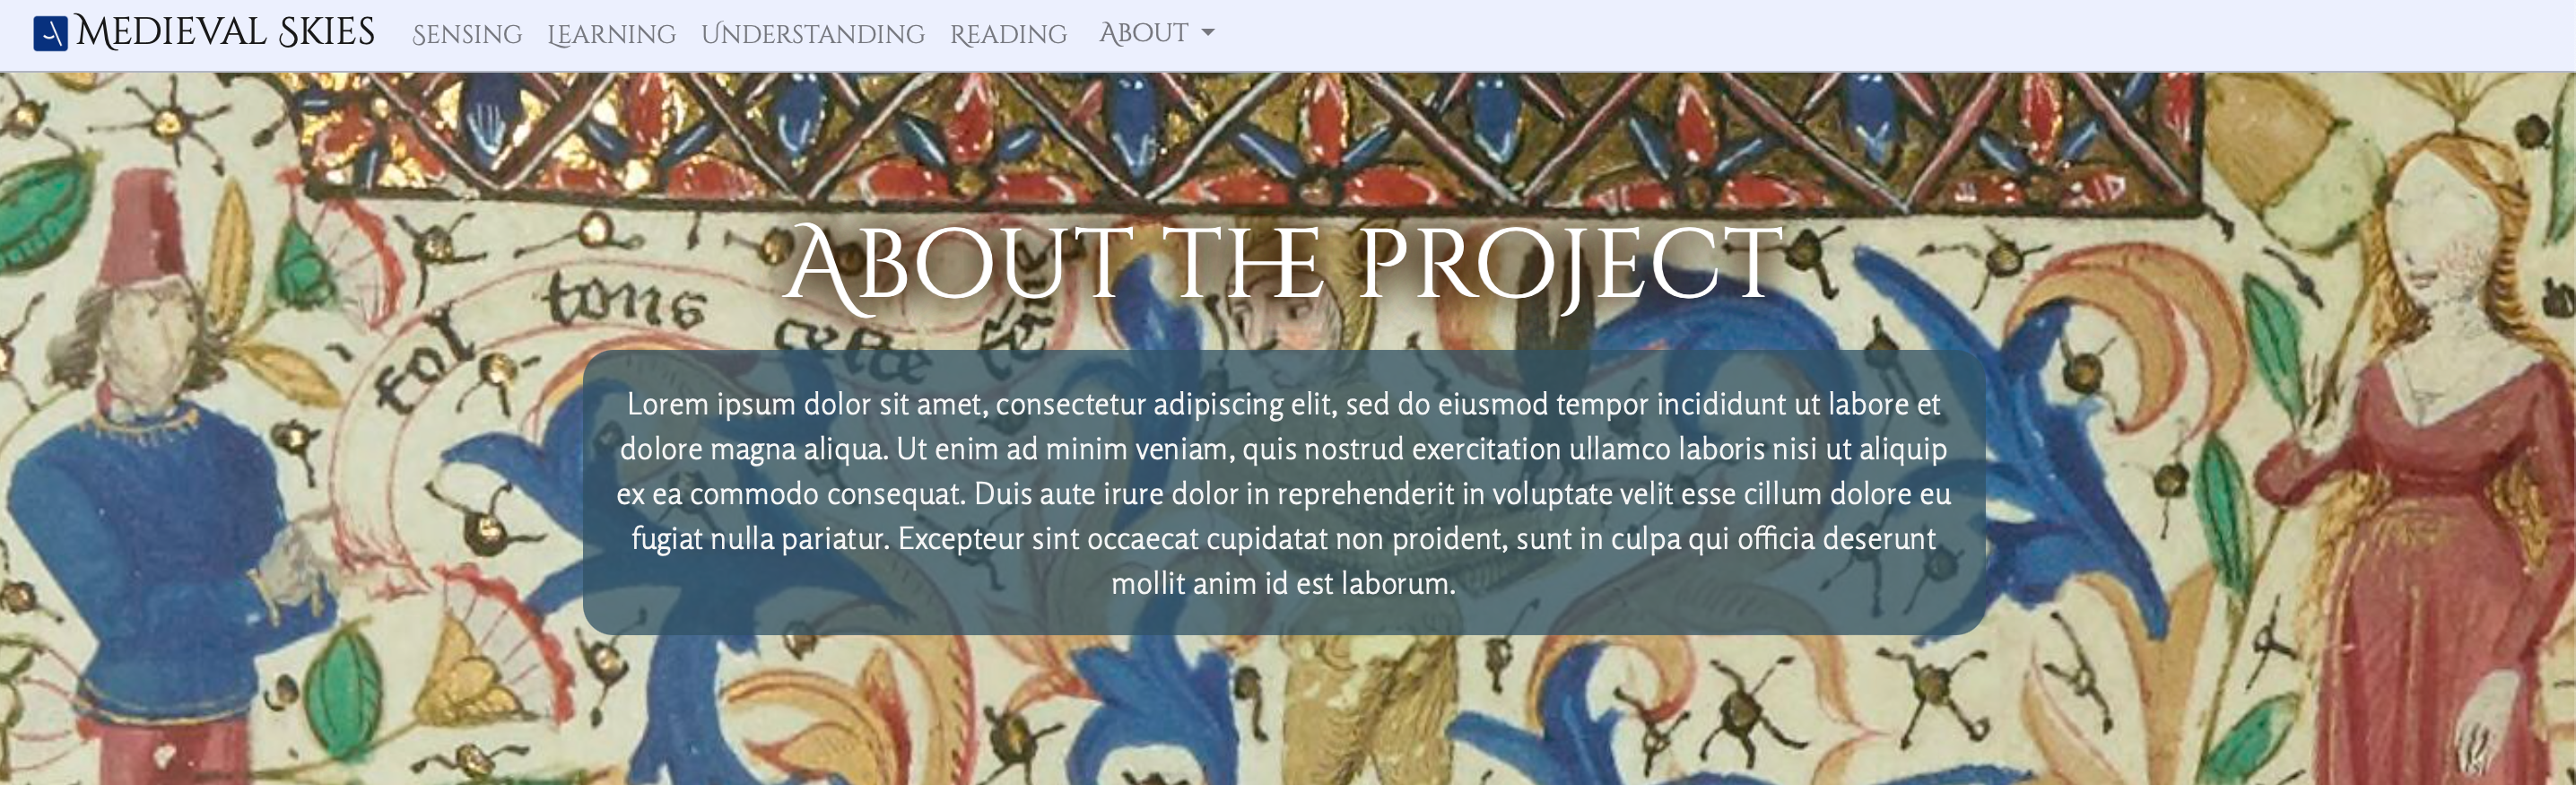
\includegraphics[width=\textwidth]{images/partie3/website/expo-about.png}
    \end{subfigure}
    \begin{subfigure}[h]{0.5\textwidth}
        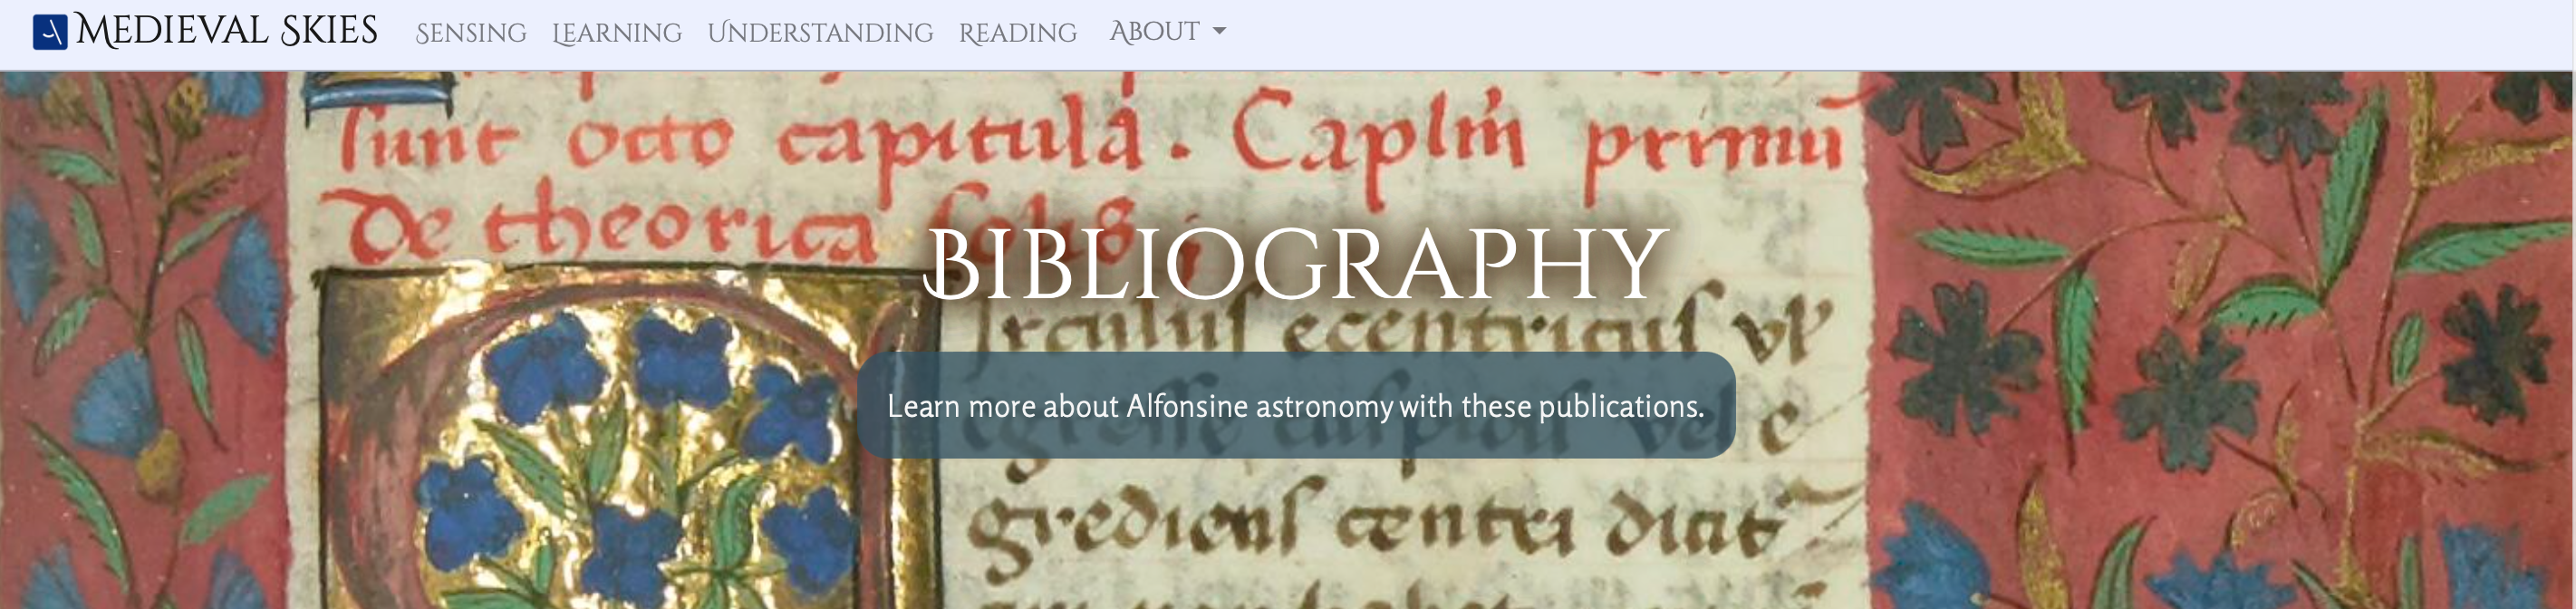
\includegraphics[width=\textwidth]{images/partie3/website/expo-bibliography.png}
    \end{subfigure}
    \begin{subfigure}[h]{0.5\textwidth}
        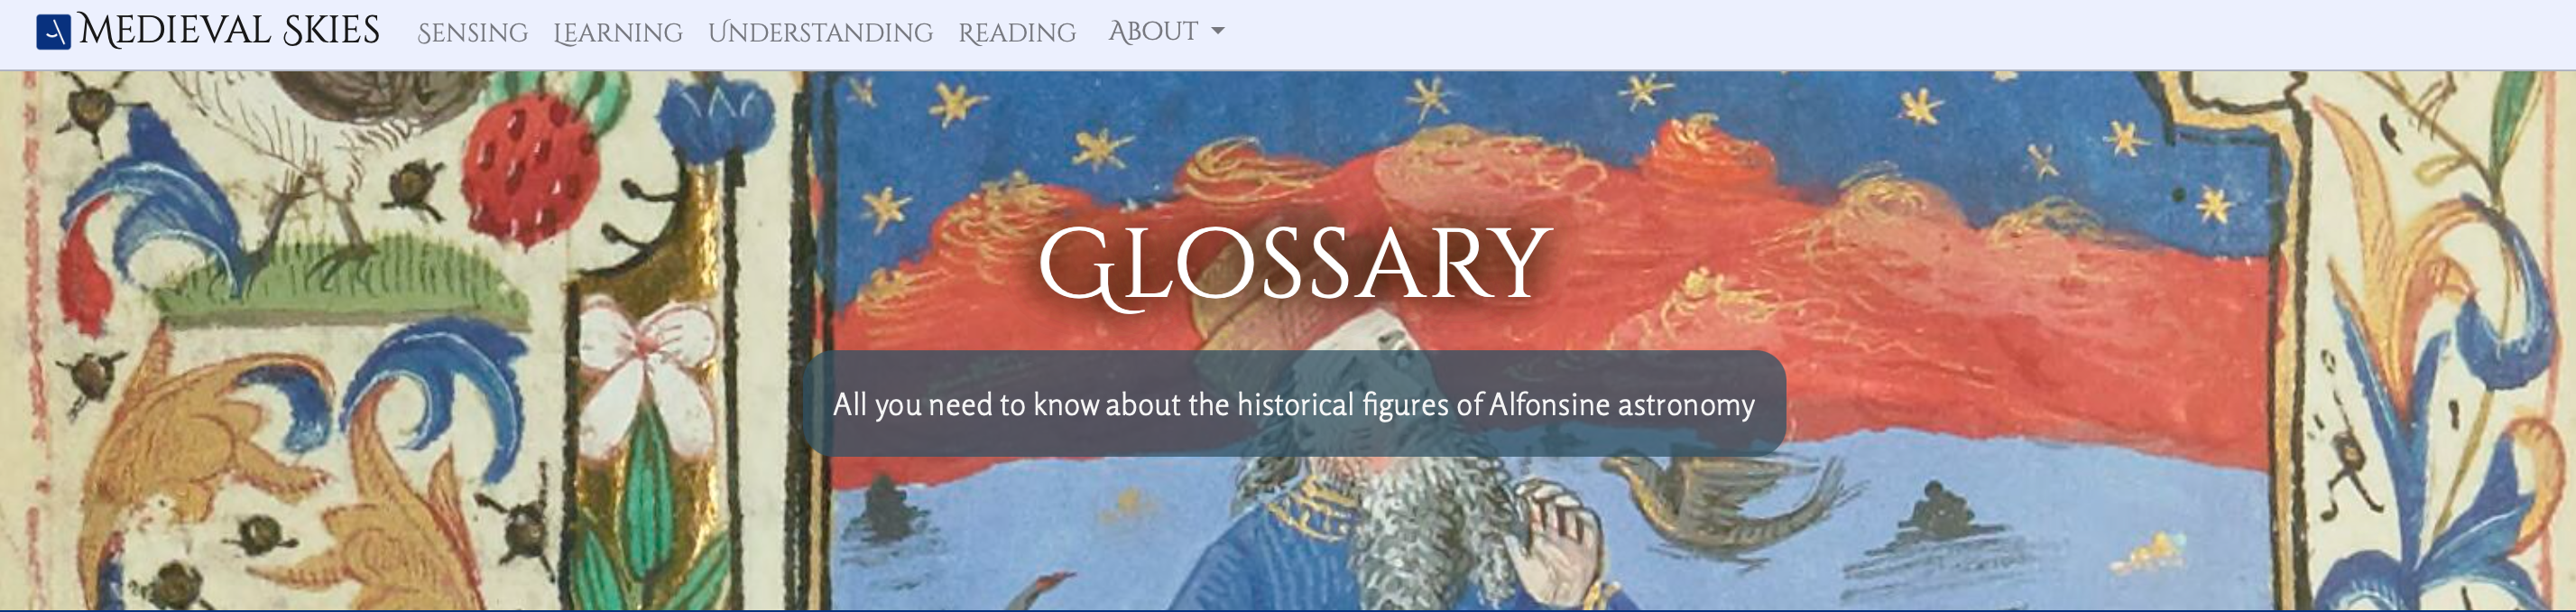
\includegraphics[width=\textwidth]{images/partie3/website/expo-glossary.png}
    \end{subfigure}
    \caption{Pages \textit{About this project}, \textit{Bibliography} et \textit{Glossary} du site \textit{Medieval skies under(book)cover}}
    \end{figure}

    \subsection{Ajouter, modifier ou supprimer des éléments}
    
    \subsubsection{Ajouter, modifier ou supprimer une page}
    On s'intéresse ici aux pages qui ne sont pas des thèmes ou des parcours, elles sont actuellement au nombre de quatre : \textit{Home}, \textit{About this project}, \textit{Bibliography} et \textit{Glossary}. Il sera possible d'en ajouter d'autres comme une page donnant accès à une carte précisant les lieux de conservation des manuscrits et ceux de production des textes qu'ils renferment, parmi les autres pages à créer on peut aussi évoquer la section jeu. L'ajout se fait en suivant quelques étapes : la première est de se rendre dans le fichier \texttt{routes.py} et d'y définir la fonction qui permettra d'inclure cette nouvelle page l'exposition. Prenons l'exemple de la page \textit{About}: 
    
    \begin{minted}{python}
    @app.route("/about", methods=["GET"])
    def about():
    return render_template(
        "pages/about.html",
         title="About",
         theme=main_pages["about"],
    )
    \end{minted}

    L'étape suivante consiste en une modification du fichier \texttt{paths.py}, il faut se rendre dans le dictionnaire appelé \texttt{main\_pages} où le nom de la page est utilisé comme clé et les informations relatives à la pages les valeurs.

    \begin{minted}{python}
    "about": {
    "url": "/about",
    "img": "static/img/cards/main-pages/about.jpg",
    "iiif": "https://gallica.bnf.fr/iiif/ark:/12148/btv1b100202503/f331/141,2291,1533,672/full/0/native.jpg",
    "header": "About this project",
    },
    \end{minted}

    Voici à quoi correspondent les différents éléments :
    \begin{itemize}
    \item \texttt{url} : \acrshort{url} de la page en cours de création
    \item \texttt{img} : image utilisée pour l'arrière plan du parallax
    \item \texttt{iiif} : lien vers l'image utilisée pour l'arrière plan du parallax au format \acrshort{iiif}
    \item \texttt{header} : titre de la page
    \end{itemize} 

    Si nécessaire, il faut ensuite ajouyter la page à la \textit{navbar} dans le fichier \texttt{navbar.html} où un élément \texttt{<a class="dropdown-item">}.

    \begin{minted}{html}
    <li class="dropdown">
        <button class="btn btn-secondary dropdown-toggle" type="button" id="dropdownMenuButton" data-toggle="dropdown" aria-haspopup="true" aria-expanded="false">About
        </button>
        <div class="dropdown-menu" aria-labelledby="dropdownMenuButton">
         <a class="dropdown-item" href="{{url_for('about')}}">About the project</a>
            <a class="dropdown-item" href="{{url_for('bibliography')}}">Bibliography</a>
            <a class="dropdown-item" href="{{url_for('glossary')}}">Glossary</a>
        </div>
    </li>
    \end{minted}

    Effectuer des modifications se fait de la même manière dans les différents fichiers mentionnés en laissant simplement de côté les étapes de création. 

    \subsubsection{Ajouter, modifier ou supprimer un thème ou un parcours}
    De façon assez analogue à l'ajout des autres pages, il faut d'abord définir une fonction dans le fichier \texttt{routes.py}. 
    
    Pour les thèmes, en prenant l'exemple du thème \textit{Sensing}\footnote{Avant d'avoir des noms définitifs pour les noms des thèmes, \textit{heritage}, \textit{historical}, \textit{scientific} et \textit{manuscripts} désignaient respectivement les thèmes \textit{Sensing}, \textit{Learning}, \textit{Understanding} et \textit{Reading}, c'est pour cette raison qu'ils sont ainsi désignés dans le code } : 
    \begin{minted}{python}
        @app.route("/heritage", methods=["GET"])
         def heritage():
            return theme_page("Heritage", "heritage", heritage_trails)
    \end{minted}
    
    Pour les parcours, avec l'exemple du parcours \textit{Seeing the manuscript} : 
    \begin{minted}{python}
        @app.route("/heritage/seeing", methods=["GET"])
        def seeing():
            return trail_page("Seeing the manuscript", "seeing", heritage_trails)
    \end{minted}
    
    Ensuite, le fichier \texttt{paths.py} doit à son tour être modifié. Pour ajouter un thème, il faut effectuer les modifications dans le dictionnaire \texttt{all\_themes}. Pour un parcours, il faut les effectuer dans le dictionnaire correspondant au thème dont fait partie ce parcours. 
    
    Pour les thèmes, en prenant l'exemple du thème \textit{Sensing} :
    \begin{minted}{python}
    "heritage": {
        "url": "/heritage",
        "img": "static/img/cards/main-pages/heritage.jpg",
        "iiif": "https://gallica.bnf.fr/iiif/ark:/12148/btv1b100202503/f459/133,1157,1262,490/full/0/native.jpg",
        "header": "Heritage trails",
        "category": "Focus on the material dimension of the manuscripts (the manuscript that we touch), on the visual aspects (the manuscript that we see) and the intellectual aspects (the manuscript that we read).",
        "color": "var(--heritage-color)",
        "parallax": "var(--parallax-heritage)",
    },
    \end{minted}
    
    Pour les parcours, avec l'exemple du parcours \textit{Seeing the manuscript} : 
    
    \begin{minted}{python}
    "seeing": {
        "url": "/heritage/seeing",
        "img": "static/img/cards/heritage/seeing.jpg",
        "iiif": "https://gallica.bnf.fr/iiif/ark:/12148/btv1b100202503/f261/159,197,322,555/800,/0/native.jpg",
        "category": "Discover",
        "header": "Seeing the manuscript",
        "color": "var(--heritage-color)",
        "exhibit": "https://www.exhibit.so/exhibits/3Ka2M3S7md6pdLZBy22C?embedded=true",
    },
    \end{minted}
    
    Les informations qui constituent les valeurs de ces dictionnaires sont tout à fait similaires qu'il s'agisse des thèmes ou des parcours : 
    \begin{itemize}
    \item \texttt{url} : \acrshort{url} de la page en cours de création
    \item \texttt{img} : image utilisée pour l'arrière plan du parallax ; l'image doit être enregistrée plutôt qu'utiliser celle au format \acrshort{iiif} car sinon le temps de chargement est bien trop important.
    \item \texttt{iiif} : lien vers l'image utilisée pour l'arrière plan du parallax au format \acrshort{iiif}
    \item \texttt{header} : titre du thème ou du parcours
    \item \texttt{category} : pour les thèmes, desciption de celui-ci ; pour les parcours, \og{}Discover\fg{} qui apparait sur les cartes
    \item \text{color} : couleur de fond de la page pour les thèmes, de fond de la section réservée au carrousel pour les parcours (la couleur utilisée est la même pour le thème et les parcours qui en font partie)
    \item \texttt{parallax} : couleur de fond du texte de description dans la section parallaax
    \item pour les parcours seulement, \texttt{exhibit} : lien vers l'\textit{exhibit} créé pour ce parcours
    \end{itemize} 
    
    Les couleurs sont définies comme variables dans le fichier \texttt{style.css}. Les thèmes doivent aussi être ajoutés à la barre de navigation afin d'être accessibles depuis l'intégralité des pages du site web. Le procédé est le même que pour les autres pages, à la différence que les thèmes ne sont pas ajoutés au menu déroulant. 
    
    \begin{minted}{html}
    <li class="nav-item">
        <a class="nav-link" href="{{url_for('heritage')}}" 
        title="Material aspect of the manuscript">Heritage</a>
    </li>
    \end{minted}
    
    Là encore, pour effectuer des modifications ou des suppression, ce sont les mêmes fichiers qui doit être retravaillés. 
    
    \subsubsection{Ajouter, modifier ou supprimer une entrée au glossaire}
    Dans ce cas, il n'y a pas de page à créer car la structure de la page \textit{Glossary} existe déjà, il s'agit simplement d'ajouter de nouvelles entrées ou de modifier celles qui sont déjà intégrées. Cela passe par le fichier \texttt{persons.py}. Dans le dictionnaire \textit{persons}, les informations liées à un personnage peuvent être ajoutées en valeurs tandis que son nom est la clé de ce couple clé/valeur :
    
    \begin{itemize}
        \item \texttt{name} : nom de l'astronome 
        \item \texttt{url} : \acrshort{url} de la page Wikipedia, si elle existe
        \item \texttt{biography} : éléments de biographie (à rédiger)
        \item \texttt{attention\_points} : folio(s) mentionnant le personnage et le lien de l'\textit{attention point} correspondant (il faut être vigilant à reporter le lien précis de l'\textit{attention point} et non pas celui qui renverrait le visiteur au début de l'\textit{exhibit}
        \item \texttt{id\_biblissima} : identifiant de l'astronome dans la base de données Biblissima, quand cette donnée est disponible
    \end{itemize}
    
    
    Illustrons cela avec la première entrée du glossaire : 
    \begin{minted}{python}
    "albumazar": {
        "name": "Abu Ma'shar",
        "url": "",
        "biography": "",
        "attention_points": {
            manuscripts_trails["bnf7281"]["header"]: {
                "f. 237v": "https://www.exhibit.so/exhibits/pByGoZQTs7Y0d5RA1EXk?screen=ywWveU59hwK7G4Aap3er"
            },
            manuscripts_trails["bnf7286c"]["header"]: {
                "f. 55r": "https://www.exhibit.so/exhibits/tPKyQQcpctVpM4tzsTnu?screen=qfI07VfoYKZX59dOJlEa"
            },
            manuscripts_trails["basel7"]["header"]: {
                "f. 82r": ""
            },
        },
        "id_bliblissima": "Q624",
    },
    \end{minted}
    
    Une fois les pages créées, il est donc aisé de modifier leur contenu. De plus quel que soit l'élément que l'on souhaite changer, les étapes à suivre sont très similaires ce qui rend la prise en main plutôt facile. 

	\section{Réalisation d’une exposition modulaire}
	Ce site est conçu grâce à une application flask. Flask est un module Python qui permet de développer des applications de manière plutôt simple. Au sein de cette application, des \textit{templates} sont utilisés pour différents éléments utilisés à plusieurs endroits. Procéder de la sorte rend la réutilisation de ces éléments simple quand elle est nécessaire. Lors de la conception de cette exposition, l'idée été de concevoir quelque chose qui puisse être modulé aisément selon les besoins, notamment pour être en mesure d'ajouter un manuscrit ou un parcours le cas échéant. Ainsi des \textit{templates} existent pour la création des pages de thèmes et de parcours mais aussi pour ajouter des carrousels, des \textit{cards} ou des \textit{exhibits}, par exemple. 
	
    \subsection{Création de fonctions}
    La création de contenu modulaire en python passe par la définition de fonctions. Pour les pages qui font appel à des \textit{templates}, ces fonctions prennent des paramètres plus nombreux comme le montre l'exemple de la fonction créée pour les pages des principaux thèmes \footnote{Les autres fonctions créées en suivant le même principe peuvent être consultées en annexe \ref{Fonctions}, à la page \pageref{Fonctions}.} :  
    \begin{minted}{python}
    def theme_page(title, theme_name, theme_trails, themes=all_themes):
        trails = list(theme_trails.values()) 
        #permet de placer les cards dans un ordre aléatoire:
        random.shuffle(trails) 
        return render_template(
            "pages/theme.html",
            title=title,
            id=theme_name,
            theme=themes[theme_name],
            cards=trails,
            #permet de retirer le thème où l'on se trouve du carrousel:
            carousel_items=remove_item(themes, theme_name),
        )
    \end{minted}
    
    Ces fonctions peuvent alors être appelées au gré des besoins et des évolutions du contenu de l'exposition. C'est le cas pour chacune des pages des principaux thèmes, ici avec l'exemple du thème \textit{Learning} :
    
    \begin{minted}{python}
    def historical():
        return theme_page("Historical", "historical", historical_trails)
    \end{minted}
    
    Si un thème vient à être ajouté, il suffira donc de créer la route dans le fichier \texttt{route.py}, comme expliqué dans la partie précédente, et de faire appel à la fonction \texttt{theme\_page}. De façon analogue, les pages des parcours font, quant à elles, appel à la fontion \texttt{trail\_page}. Là encore, pour ajouter un parcours les seules exigences sont la création de la route et l'appel de la fonction. 
    
	\subsection{Création de \textit{templates}}
	Une fois les fonctions en place, il est nécessaire de fournir le code \acrshort{html} qui permettra d'afficher le contenu sur le navigateur des visiteurs. Là encore, plutôt que de créer un fichier \acrshort{html} pour chacune des pages de l'exposition, le contenu commun a été mutualisé, sur les conseils de Ségolène Albouy. Cela constitue une bonne pratique qui permet de rendre le code plus clair et plus propre et qui facilite également sa modification et sa prise en main par des tiers. Ainsi des \textit{templates} ont, une fois de plus, été créés pour les pages de thèmes et de parcours. \footnote{L'ensemble des \textit{templates} utilisés pour le développement de l'interface de l'exposition fait partie des livrables techniques}.
	
	Au sein de ces \textit{templates} principaux, d'autres, plus petits car relatifs à un élément de la page plutôt qu'à son architecture complète, sont appelés et concernent notamment des éléments \acrshort{css} tels que les carrousels présents en bas de ces pages pour accéder aux autres thèmes ou autres parcours, les \textit{cards} qui permettent aux visiteurs de choisir un parcours au sein d'un thème ou encore les parallax qui sont la section supérieure de l'ensemble des pages du site où l'on trouve le titre et une description sommaire du contenu de la page. 
	De même pour les parcours, l'insertion des \textit{exhbits} se fait par le biais d'un \textit{template}. Pour la création du glossaire, c'est encore une fois ce même système qui est mis en place. 
	
	Les éléments à afficher sur les pages présentant un contenu similaire sont renseignés dans des dictionnaires regroupés dans le fichier \texttt{utils}. Le fait d'avoir des dictionnaires permet d'utiliser des boucles pour que le contenu associé à chacun des éléments soit affiché correctement mais en ayant seulement quelques lignes de code plutôt qu'un code très long avec un fichier \acrshort{html} pour chaque page qui contiendrait des répétitions nombreuses des mêmes morceaux de code. Ainsi, un \textit{template} utilisant une boucle indiquant ce qui doit être affiché pour chaque parcours dans le dictionnaire relatif à un thème est préférable à la répétition quatre fois, si il y a quatre parcours, d'un code identique dans sa structure mais où le contenu est spécifique à chaque parcours. Procéder ainsi permet enfin d'éviter, ou au moins de réduire, les erreurs qui se glisseraient inévitablement dans un code construit de la sorte. 
	
	\chapter{Mise en valeur des données}
	Dans cet ultime chapitre, on s'efforce de porter un regard critique sur la mise en valeur des données de la recherche grâce à l'exposition \textit{Medieval skies under(book)cover} en évoquant des questionnements sur le rendu esthétique du site web avant de dire quelques mots du futur de l'exposition.
	\section{Une interface au service des visiteurs}
	\subsection{Création d'une exposition \textit{responsive}}
	Un site web \textit{responsive} est un site qui peut s'accommoder à toutes les tailles et résolutions d'écran. Il s'agit d'adapter l'affichage des éléments d'une pages aux différents supports que les visiteurs peuvent utiliser : ordinateurs, tablettes et \textit{smartphones}. Le contenu n'est donc pas propre à chaque support mais il est adapté à chacun d'entre eux.  À l'heure où l'utilisation des \textit{smartphones} est omniprésente, il semble important de pouvoir proposer un contenu auquel les visiteurs pourront avoir accès depuis leur \textit{smartphones}. En effet, ne pas considérer cette possibilité serait exclure dès le départ une partie du public ciblé qui cherche a avoir accès à un contenu instantané. 
	
	À l'échelle globale du site web, l'affichage du contenu des pages est harmonisé pour les différentes tailles d'écrans dans le fichier \texttt{style.css} : 
	\begin{minted}{css}
	@media screen and (min-width: 900px) {
        .page-title {
            font-size: 4rem;
        }
        .main-content {
         max-width: 40vw;
        }
        .main-item {
            width: 55vw;
        }
        .div-main-content {
            height: 40vw;
        }
    }

    @media screen and (min-width: 500px) and (max-width: 900px) {
        .page-title {
            font-size: 5rem;
        }
        .main-content {
            max-width: 80vw;
        }
        .main-item {
            width: 85vw;
        }
        .div-main-content {
            height: 81vw;
        }
        #parallax-title {
            font-size: xxx-large;
        }
    }

    @media screen and (max-width: 500px) {
        .page-title {
            font-size: 10vw;
        }
        .main-content {
            max-width: 90vw;
        }
        .main-item {
            width: 90vw;
        }
        .div-main-content {
            height: 92vw;
        }
        .add-lg {
            display: none;
        }
        #parallax-title {
            font-size: xx-large;
        }
    }
	 \end{minted}
	 
	 Il est ainsi possible de paramétrer l'affichage des titres et du contenu selon selon la taille des écrans, pour avoir un résultat le plus adapté possible, on définit trois tailles d'écran qui correspondent plus ou moins aux ordinateurs, tablettes et \textit{smartphones}.
	 Néanmoins, pour des écrans de petite taille, il n'est pas exclu de faire le choix de pas afficher certains éléments : c'est le cas sur la page \textit{Glossary} pour les \textit{smartphones} où le listing des folios n'apparaît pas pour privilégier le contenu biographique\footnote{Une comparaison des trois écrans est disponible en annexe \ref{ResponsiveScreen}, à la page \pageref{ResponsiveScreen}.}. De la même manière, sur les pages des thèmes, le nombre de cartes affichées sur une même ligne varie selon la taille de l'écran. Ces paramètres sont à régler dans le \acrshort{css} du fichier à l'intérieur de la balise \texttt{<style>}.

    Néanmoins, malgré ces efforts il faut noter que tous les contenus ne sont pas parfaitement adaptés à tous les types d'écran. Par exemple, sur la page d'accueil, un manuscrit cliquable a été ajouté en utilisant une image vectorielle. Malgré des difficultés de calibrage du \acrshort{svg} pour que les zones cliquables correspondent aux bonnes coordonnées de l'image quelle que soit la taille de l'écran, ce problème a pu être résolu. Toutefois, demeure le fait que sur un écran tactile le visiteur n'a pas d'indication sur cette fonctionnalité alors que sur un écran non tactile, au survol de la souris la zone cliquable est grisée : cela indique au visiteur que c'est une zone cliquable.  

    \subsection{Réflexion sur l'esthétique du site web}
    Si le principal élément de mise en valeur des manuscrits vient des \textit{exhibits}, cela n'exclue pas le reste du site web d'y contribuer. En effet, l'objectif est donc de permettre aux visiteurs d'avoir une progression fluide jusqu'à la navigation au sein d'un \textit{exhibit} et donc d'un parcours. 
    Un code couleur très simple aide les visiteurs à se repérer dans leur navigation : la couleur principale utilisée pour un thème est également présente sur les pages des parcours issus de celui-ci. Cela aide les internautes à déambuler dans cette exposition en sachant rapidement que les pages qu'ils consultent sont ou non associées. Pour être bien sûre que les couleurs utilisées soient identiques quand elles doivent l'être des variables ont été créées afin de réutiliser très commodément ces couleurs lors de l'implémentation du \acrshort{css} des différents éléments des pages web. 
    
    \begin{minted}{css}
    --heritage-color: #518cb0;
    --parallax-heritage: rgba(55, 78, 113, 0.75);
    --historical-color: #757055;
    --parallax-historical: rgba(48, 52, 41, 0.75);
    --scientific-color: #dcccb5;
    --parallax-scientific: rgba(62, 51, 42, 0.75);
    --manuscripts-color: #862b28;
    --parallax-manuscripts: rgba(99, 26, 21, 0.75);
    \end{minted}
    
    La couleur étant un élément de cohérence, les couleurs choisies pour chacun des thèmes renvoient à celles du manuscrit \acrshort{svg} de la page d'accueil : dès le départ, le visiteur peut donc associer une couleur à une thématique. De plus, lors de l'ajout des \textit{shortcuts}, on peut envisager l'utilisation de ces mêmes couleurs pour signaler au vsiteur qu'il est conduit vers une autre thématique.
    
    Par ailleurs, pour les pages considérées comme annexes, dans le sens où elles ne concernent pas les parcours d'exposition, la couleur qui a été choisie est la nuance de bleu qui est utilisée sur d'autres site web du projet \acrshort{alfa} afin de, là aussi, créer de la cohérence à l'échelle globale du projet. \\
    
    Enfin, pour fluidifier la progression au sein de l'exposition, des titres clairs ont du être choisis pour les thèmes majeurs mais également pour l'exposition elle-même. Autre preuve du dialogue entre les différentes personnes prenant part au projet, tous ceux qui le souhaitaient ont pu proposer des titres qui ont ensuite été soumis à un vote parmi les membres de l'équipe. Ces titres devaient satisfaire les besoins scientifiques de clarté pour aiguiller les visiteurs tout en se pliant à des contraintes techniques, voire esthétiques, d'intégration au site web. Ainsi, le titre devait pouvoir avoir une version courte pour la barre de navigation. De même les titres des thèmes devant également être ajoutés à la \textit{navbar}, ils ne devaient pas non plus être trop longs, idéalement un seul mot.

	\section{Futur de cette exposition virtuelle}
	Si l'objectif d'avoir une interface d'exposition est atteint, cela ne signifie pas que ce projet de \textit{digital exhibition} est pour autant achevé. Premièrement, un certain nombre d'\textit{attention points} est encore à compléter. Ensuite doivent être envisagés l'ajout des parcours raccourcis, avec la sélection des \textit{attention points} qui en feront parti, et le choix des \textit{must see}. Le cas du manuscrit de l'Université de Bâle, disponible uniquement sous microfilms, doit aussi être statué car, en l'état, il ne peut être inclus à une exposition virtuelle. Les pages annexes devront aussi être complétées afin d'offrir aux internautes l'intégralité des ressources utiles à leur compréhension de l'astronomie alphonsine. Tout cela correspond à des points connus de l'équipe et leur réalisation est déjà prévue. 
	
	D'autre part, on peut également penser à des idées de plus grande envergure pour compléter cette première version de l'exposition. Un premier projet dont il est déjà question est de proposer aux internautes de visiter l'exposition \textit{Medieval skies} dans une autre langue que l'anglais. Le caractère international de l'équipe offre des possibilités pour le français, l'italien ou encore l'espagnol. Cela signifierait aussi une expansion de l'audience. En effet, si nombreuses sont les personnes qui peuvent comprendre l'anglais, avoir la possibilité de bénéficier de cette expérience dans sa langue maternelle serait une valeur ajoutée à l'exposition. De plus, le contenu de l'exposition a pu être évoqué comme possible complément d'un contenu pédagogique lié au programme scolaire et, là encore, la possibilité d'y accéder dans d'autres langues que l'anglais serait bienvenue. 
	
	Enfin, ce projet peut facilement être augmenté par l'ajout d'autres manuscrits ou d'autres parcours grâce à l'utilisation de \textit{templates}. Cette éventualité prendrait place au sein du projet \acrshort{alfa} mais ce n'est pas la seule possibilité. En effet, on peut aussi imaginer une vie en dehors de l'Observatoire de Paris, pour l'exposition peut-être mais pour son modèle plutôt. Ainsi, du fait de son architecture simple, facilement prise en main et aisément adaptable, \textit{Medieval skies under(book)cover} pourrait servir de modèle à une autre exposition qui serait construite de façon analogue avec des thèmes subdivisés en plusieurs parcours. Cela irait dans le sens des humanités numériques comme facteur de partage, de collaboration et de science ouverte. \\
	
	Cette ultime partie consacrée au développement effectif d'une interface permettant la mise en valeur du corpus alphonsin a permis de mettre en avant le dynamisme de la communauté \acrshort{iiif} et l'intérêt de ces images haute définition pour exposer de précieux manuscrits. Pour développer le site web, le choix a été fait d'une architecture simple et facilement modulable afin de rendre la réutilisation du code la plus simple posisble. Enfin, une réflexion a été portée sur la mise en valeur des données et les possibles axes d'amélioration pour le futur. 



	\chapter*{Conclusion}
	\addcontentsline{toc}{chapter}{Conclusion}
	Ce mémoire s'est efforcé de décrire le travail réalisé au cours du stage effectué au sein de l'équipe du projet de recherche \acrshort{alfa}, à l'Observatoire de Paris. Le principale mission était la scénographie d'une exposition virtuelle d'un corpus de manuscrits issus de l'astronomie alphonsine, courant scientifique européen qui se développe entre les XIIIe et XVIe siècles. Après avoir développé la plateforme \acrshort{dishas} pour valoriser les données produites dans le cadre de ce projet de recherche et conçu des outils comme le \textit{survey} ou \textit{Table transcriber}, l'équipe avait à cœur de mettre en scène une exposition. Les humanités numériques ayant une place de choix dans le projet \acrshort{alfa}, se tourner vers une exposition en ligne faisait sens, d'autant plus que la plupart des manuscrits sélectionnés pour en faire partie sont disponibles sous un format numérique. \\
	
	Plusieurs étapes se sont succédées pour aboutir à la création d'une plateforme d'exposition virtuelle accessible au public : une phase d'analyse, une phase de rédaction, une phase d'exécution, une phase de documentation et une phase de mise en production. \\
	
	La première partie du présent mémoire se rapporte ainsi plutôt aux premières phases d'analyse et de rédaction. En effet, après avoir pris connaissance du contexte et des principaux enjeux du projet, un important travail de reprise des données produites par les chercheurs a été effectué en vue de leur harmonisation et de leur réutilisation. C'est dans ce même temps qu'on pu être listées les exigences en matière de contenu sur le futur site web et qu'une réflexion a pu être entamée sur la définition à donner à l'objet d'exposition virtuelle. 
	
	La seconde partie touche, quant à elle, à la scénographie de façon concrète. En effet, les enjeux liés à l'expérience des visiteurs sont essentiels : la navigation au sein des différents parcours doit permettre un accès au contenu du corpus alphonsin. C'est aussi l'occasion de réfléchir au rôle des ingénieurs numériques dans un projet de recherche qui fait dialoguer considérations scientifiques et contraintes techniques et à leur mission de médiation entre les deux. Du fait de cette mission, la rédaction de documentation à destinations des chercheurs comme des ingénieurs a également occupé une place importante au cours de ce stage.
	
	Enfin, le descriptif et l'analyse du développement de l'interface viennent clore ce mémoire. L'utilisation du protocole \acrshort{iiif} a tenue une place de premier plan pour la mise en avant des numérisations. De plus, développer une plateforme \textit{responsive} et réutilisable était au centre des préoccupations afin de pouvoir concilier les besoins des utilisateurs et la recherche \textit{open source}. La proprification du code et des données est un moyen de mettre en valeur le travail des chercheurs, qui a lui-même pour objectif de dévoiler aux yeux d'un public plus large le corpus alphonsin. \\
	
	Ce stage a été une expérience très enrichissante du fait des connaissances acquises d'un point de vue technique mais également pour la découverte de ce corpus d'histoire de l'astronomie. De plus, avoir la possibilité d'évoluer dans un projet international est formateur pour aborder un milieu où l'anglais fait partie du bagage requis. \\
	
	La médiation numérique offre donc des possibilités grandissantes qui permettent de s'affranchir des barrières spatiales pour la réalisation d'une exposition. En effet, les œuvres mises en scène peuvent venir des quatre coins du monde et rester à l'abri dans leur lieu de conservation. De même, les visiteurs peuvent, depuis chez eux, accéder à de riches contenus. Malgré les avancées réalisées au cours de ce stage, de nombreuses possibilités restent à explorer pour parfaire la mise en lumière de ces manuscrits qui révèlent la richesse de l'astronomie alphonsine. 

	
	%les annexes
	\appendix
	
	\renewcommand{\appendixpagename}{Annexes}
	% permet de  renommer en "Annexes" la page de titre "Appendices"
	
	\renewcommand{\appendixtocname}{Annexes}
	% permet de renommer en "Annexes" le nom des annexes dans la table des matières
	
	\addappheadtotoc % permet d'ajouter les annexes à la table des matières
	
	\appendixpage % petmet de créer une page de titre pour les annexes

    	\chapter{\label{APcommuns}\textit{Attentions points} communs}
	Ce tableau, réalisé pour venir en aide aux chercheurs lors de l'élaboration de \textit{shortcuts} et \textit{must see}, présente pour la totalité des manuscrits de l'exposition les liens précis des \textit{attention points} tout en indiquant le nombre de parcours dans lesquels ils apparaissent.
	\begin{landscape}
		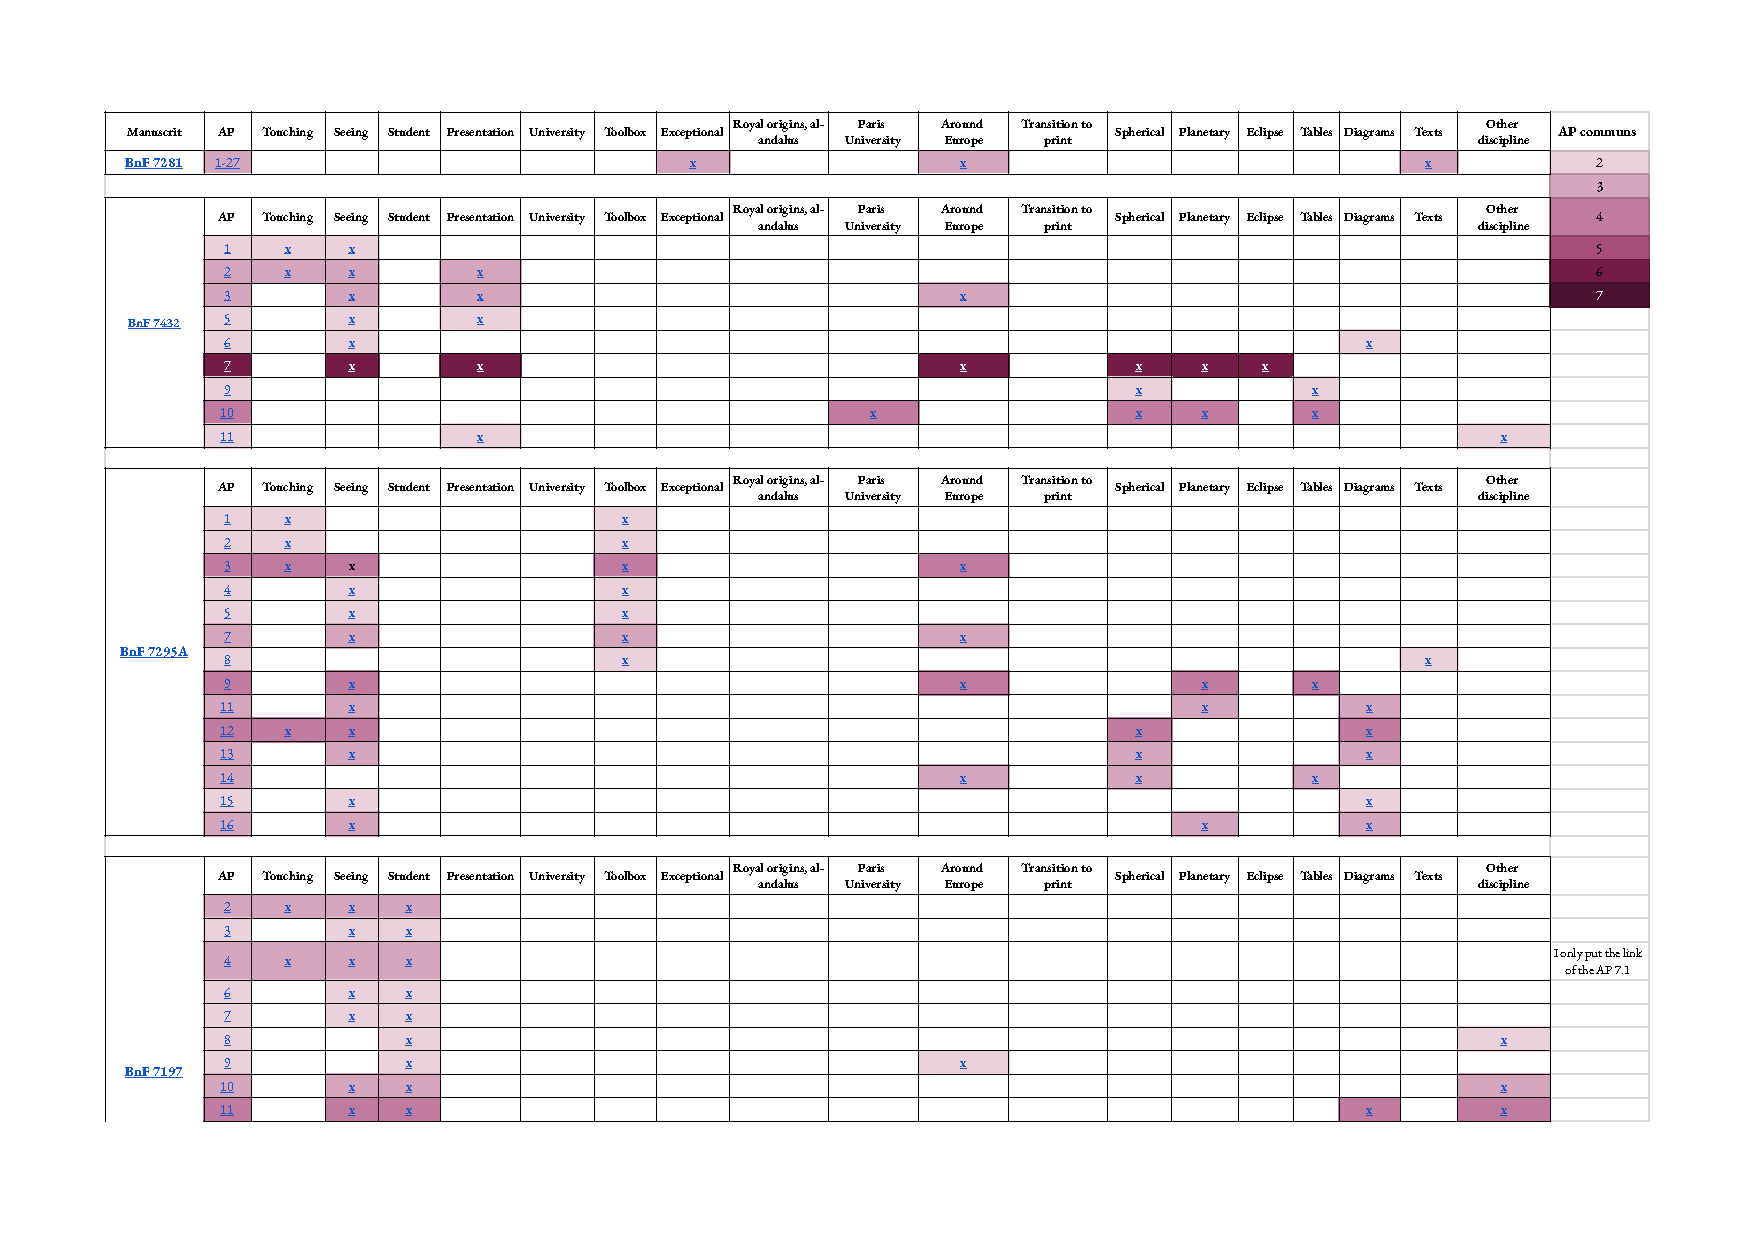
\includepdf[pages=-, scale=1,landscape=true]{annexes/APcommuns.pdf}
	\end{landscape}
	

	
    
    \include{annexes/Séminaires}
    	\chapter{\label{Tutoriel}Tutoriel Exhibit}
	\subsubsection{Find or create an Exhibit}
    Work directly on the Exhibit link that you’ll find in the third column here. The links found in this column are the one that will be used to make the improvements. For some of the paths, some modifications have already been made but mostly to try and see what could be made. The easier way to work is probably to begin with the manuscripts' paths rather than the thematic ones. Indeed, once the first category is done, you’ll be able to simply copy and paste the attention points as they’ve been improved in the specific paths they are part of (you’ll maybe have to add captions or do divide them but at least a part of the work will already be done). 
    You can also create a new Exhibit here if you want to add a new path to the exhibition. 

	\subsubsection{Complete the settings}
    If you create a new Exhibit, you land directly on the settings page. Otherwise, on the edit page of an Exhibit that already exists, the settings can be accessed and modified by clicking on the small pen at the top right corner of the box that contains the title and the description. 
    Then you can:
    \begin{itemize}
    \item select the quiz template if it is not already done
    \item modify the title
    \item complete or modify the authors list (for some I didn’t know the last names so I just wrote the first name followed by a question mark…)
    \item write or complete the description of the path (I only translated what had been written here so something else might have to be written, my translations have to be corrected because I left some things in French when I didn't know the proper way to translate…). The length of the text is limited to 1000 characters(for example, the University manuscript path description is too long so it has to be shortened.
    \item write an optional “Quiz Complete Message”: it is possible to have links in the message so an idea could be to allow the visitors to go to another path through this message 
    \item the “Rights” section is optional but maybe the libraries where the manuscripts are kept should be mentioned here ? 
    \item keep the “Access” as it is with the “Public” selected 
    \item keep the “Allow Duplication” selected as well, at least for now that it might still be useful to create shortcuts but this would probably have to be unselected when all the work is done 
    \item select “Je ne suis pas un robot” and “I have read and agree…”
    \item click on the “Update” button
    \end{itemize}

    \subsubsection{Add a manifest to the Exhibit}
    When you create a new exhibit, you need to add one or more manifest(s) but you can add a manifest later as well. Either way, you can do that by clicking on the “+ Add Item” purple button at the bottom left corner of the page. A little window will open where you can add a IIIF Manifest URL and then click on the “Import” button to be able to use it in your exhibit. When you want to use a manifest to add a new attention point, you need to select it in that same window and click on the “Add to exhibit” button. When adding a new attention point, be careful to have the corresponding manifest selected. 

    \subsubsection{Add a caption}
    At the bottom of the edit page, you will find a “+” button that you’ll have to click on in order to add an item to the exhibit. When doing so, be careful to have the right manifest selected. You can then write a caption and edit it, you can choose your image in the right part of your screen. 
    For some of the items I created, there was no caption and/or no folio indication so there are some empty captions that you can fill and the images are not always the right one because if you don’t choose an image the image that will appear is either the first of the manifest or the one used in the previous item, that explains why some folios appear more than one time when there is an empty attention points so when completing an attention point don’t forget to add the correct folio if it is not already the case. 
    Divide the caption when needed
    Some of the attention points are too long and need to be divided. That also allows more precise zooms on the concerned folios.

    Example : ms BnF 7295A AP5
    This is the attention point as it was written. Since it is only one section in Exhibit, it can only be associated to a single folio with a single zoom. Dividing the caption in different sections allows to have as many zoomed images as there are sections so the zooms are more precise and more related to the text next to them. 

    In some cases, when an attention point is used in several paths, the entirety of the caption is not needed for all said paths and it would make the storytelling and navigation easier to only keep the part actually related to the current path.  

    Example : ms 7432 AP1
    Here dividing the caption allows for better zooms but it is also good to keep only the part one would be interested in when following a specific path. Indeed, this attention point is related to both seeing and touching paths but the part about the binding is only relevant for the touching one where the part about the modern numbering is all about seeing : a good solution is to divide the caption and keep what is needed for the path. For the path related to the whole manuscript, it is also better to divide because it allows a zoom on the binding and one on the numbering. 


    \subsubsection{Add questions/quizzes}
    Using the quizz template in Exhibit allows you to add questions to the captions. Indeed, as you would enter the text of the attention points, you can write a question and then add the possible answers. The small checkbox next to the correct one has to be selected. This is a possibility to add small games in the exhibition :)

    Highlight some parts of the attention points
    These highlights in bold letters are here for the audience to easily catch the more important information of the caption.

    \subsubsection{Add pinpoints}
    In order to help the visitor know where to look on a folio, pinpoints can be added. When you click on a caption, you are able to make modifications to it through the “Question” section, next to it is another one named “Pinpoints”. In this second section, you can simply double click anywhere on the image to create a pinpoint. You can add a label to your pinpoint if you want but it will not appear on the image. 

    \subsubsection{Translate and harmonize the use of italic and quotation marks}
    Some parts of the captions are quotes from the manuscripts so they are in Latin : some of them are accompanied by a translation, some of them are not. We can think that most of the audience won’t be latin experts so a translation for all the latin will be great. 
    The translations have to be harmonized : 
    \begin{itemize}
        \item write the Latin titles in italic letters with a capital letter at the beginning
        \item the Latin quotes between quotation marks in the main text
        \item the translation in parentheses for all the Latin except for the titles
    \end{itemize}

    \subsubsection{Change the order of the attention points in a path}
    In the thematic paths, the attention points are following each other manuscript by manuscript which is probably not the best way to do it. This change can be done with drag and drop in Exhibit to have a more coherent order in terms of storytelling. 

    Example : touching the manuscript 
    An idea could be to begin with all the attention points related to bindings and from that to go further inside the manuscripts to end with the added leaflets for example. 

    \subsubsection{Find titles}
    For now the titles are those used here. For some captions (manuscript 7295A) titles have also been added. It could be a good thing to have titles for the other captions, at least to “group” the attention that are about a similar subject. 

    Example : touching the manuscript 
    Here I grouped attention points related to the bindings of the manuscripts under a common title “Binding” (that title is not the best…). 

    \subsubsection{Add links in the captions}
    These links point the audience to the Exhibits related to the folios/manuscripts mentioned in the attention point. Links for a precise slide of the Exhibit are now available later so we will  be able to include those in the exhibition. The links will have to be added once the attention points are finished.  
    Links can be added in the “Quiz Complete Message” section of the settings too. 
    Since there is a different color for each of the main themes of the exhibition, an idea is to have a colored emoji with the link to help the visitors in their navigation on the website. 

    \subsubsection{Duplicate an exhibit}
    That is a functionality that might be useful when doing the shortcuts for the longer paths. Indeed it is possible to duplicate an exhibit and then in this duplicated version to delete the attention points that will not be part of the shortcut. 
    In order to duplicate an exhibit, one must click on the “Preview” button at the bottom of the edit page and then on the “Duplicate” button in the page that will be opened. After that, you can edit the duplicate exhibit as any other exhibit, beginning with the settings. 
    When all this work is done maybe allowing duplication won’t be something to keep. To change that, the one thing to do is to uncheck the “Allow Duplication” button in the settings. 

    \subsubsection{Complete the AP that are not written or not complete or indicate if they are not to be included in the end}
    For several manuscripts, there are empty attention points listed in the column named “AP to complete” of this document so they can be written. If it was decided not to include some of those attention points, it could be good to indicate it.

    \subsubsection{Keep the links}
    When you create a new exhibit, be careful to keep the edition link to be able to find and edit your exhibit later. The best practice would probably be to add a new line to this table for all new paths and to keep all the links and information in one place. 



    \include{annexes/Spécifications}
    	\chapter{\label{Fonctions}Création de fonctions}
	
	\section{Fonction trail\_page}
	\begin{minted}{python}
    def trail_page(title, trail_name, trails):
            return render_template(
            "pages/trail.html",
            title=title,
            id=trail_name,
            trail=trails[trail_name],            
            #permet de retirer le parcours où l'on se trouve du carrousel:
            carousel_items=remove_item(trails, trail_name),
        )
    \end{minted}
    
	\section{Fonction glossary}
	\begin{minted}{python}
    def glossary():
        list_persons = sorted(persons.values(), key=lambda d: d["name"])
        return render_template(
            "pages/glossary.html",
            title="Glossary",
            persons=list_persons,
            theme=main_pages["glossary"],
        )
    \end{minted}
    
	\section{Fonction bibliography}
    \begin{minted}{python}
    def bibliography():
        list_books = sorted(books.values(), key=lambda d: d["author"], reverse=False)
        list_articles = sorted(articles.values(), key=lambda d: d["author"])
        return render_template(
            "pages/bibliography.html",
            title="Bibliography",
            books=list_books,
            articles=list_articles,
            theme=main_pages["bibliography"],
        )
    \end{minted}

    	\chapter{\label{ResponsiveScreen}\textit{Responsive screen}}
	
	\begin{figure}[!h]
    \centering
    \begin{subfigure}[h]{0.8\textwidth}
        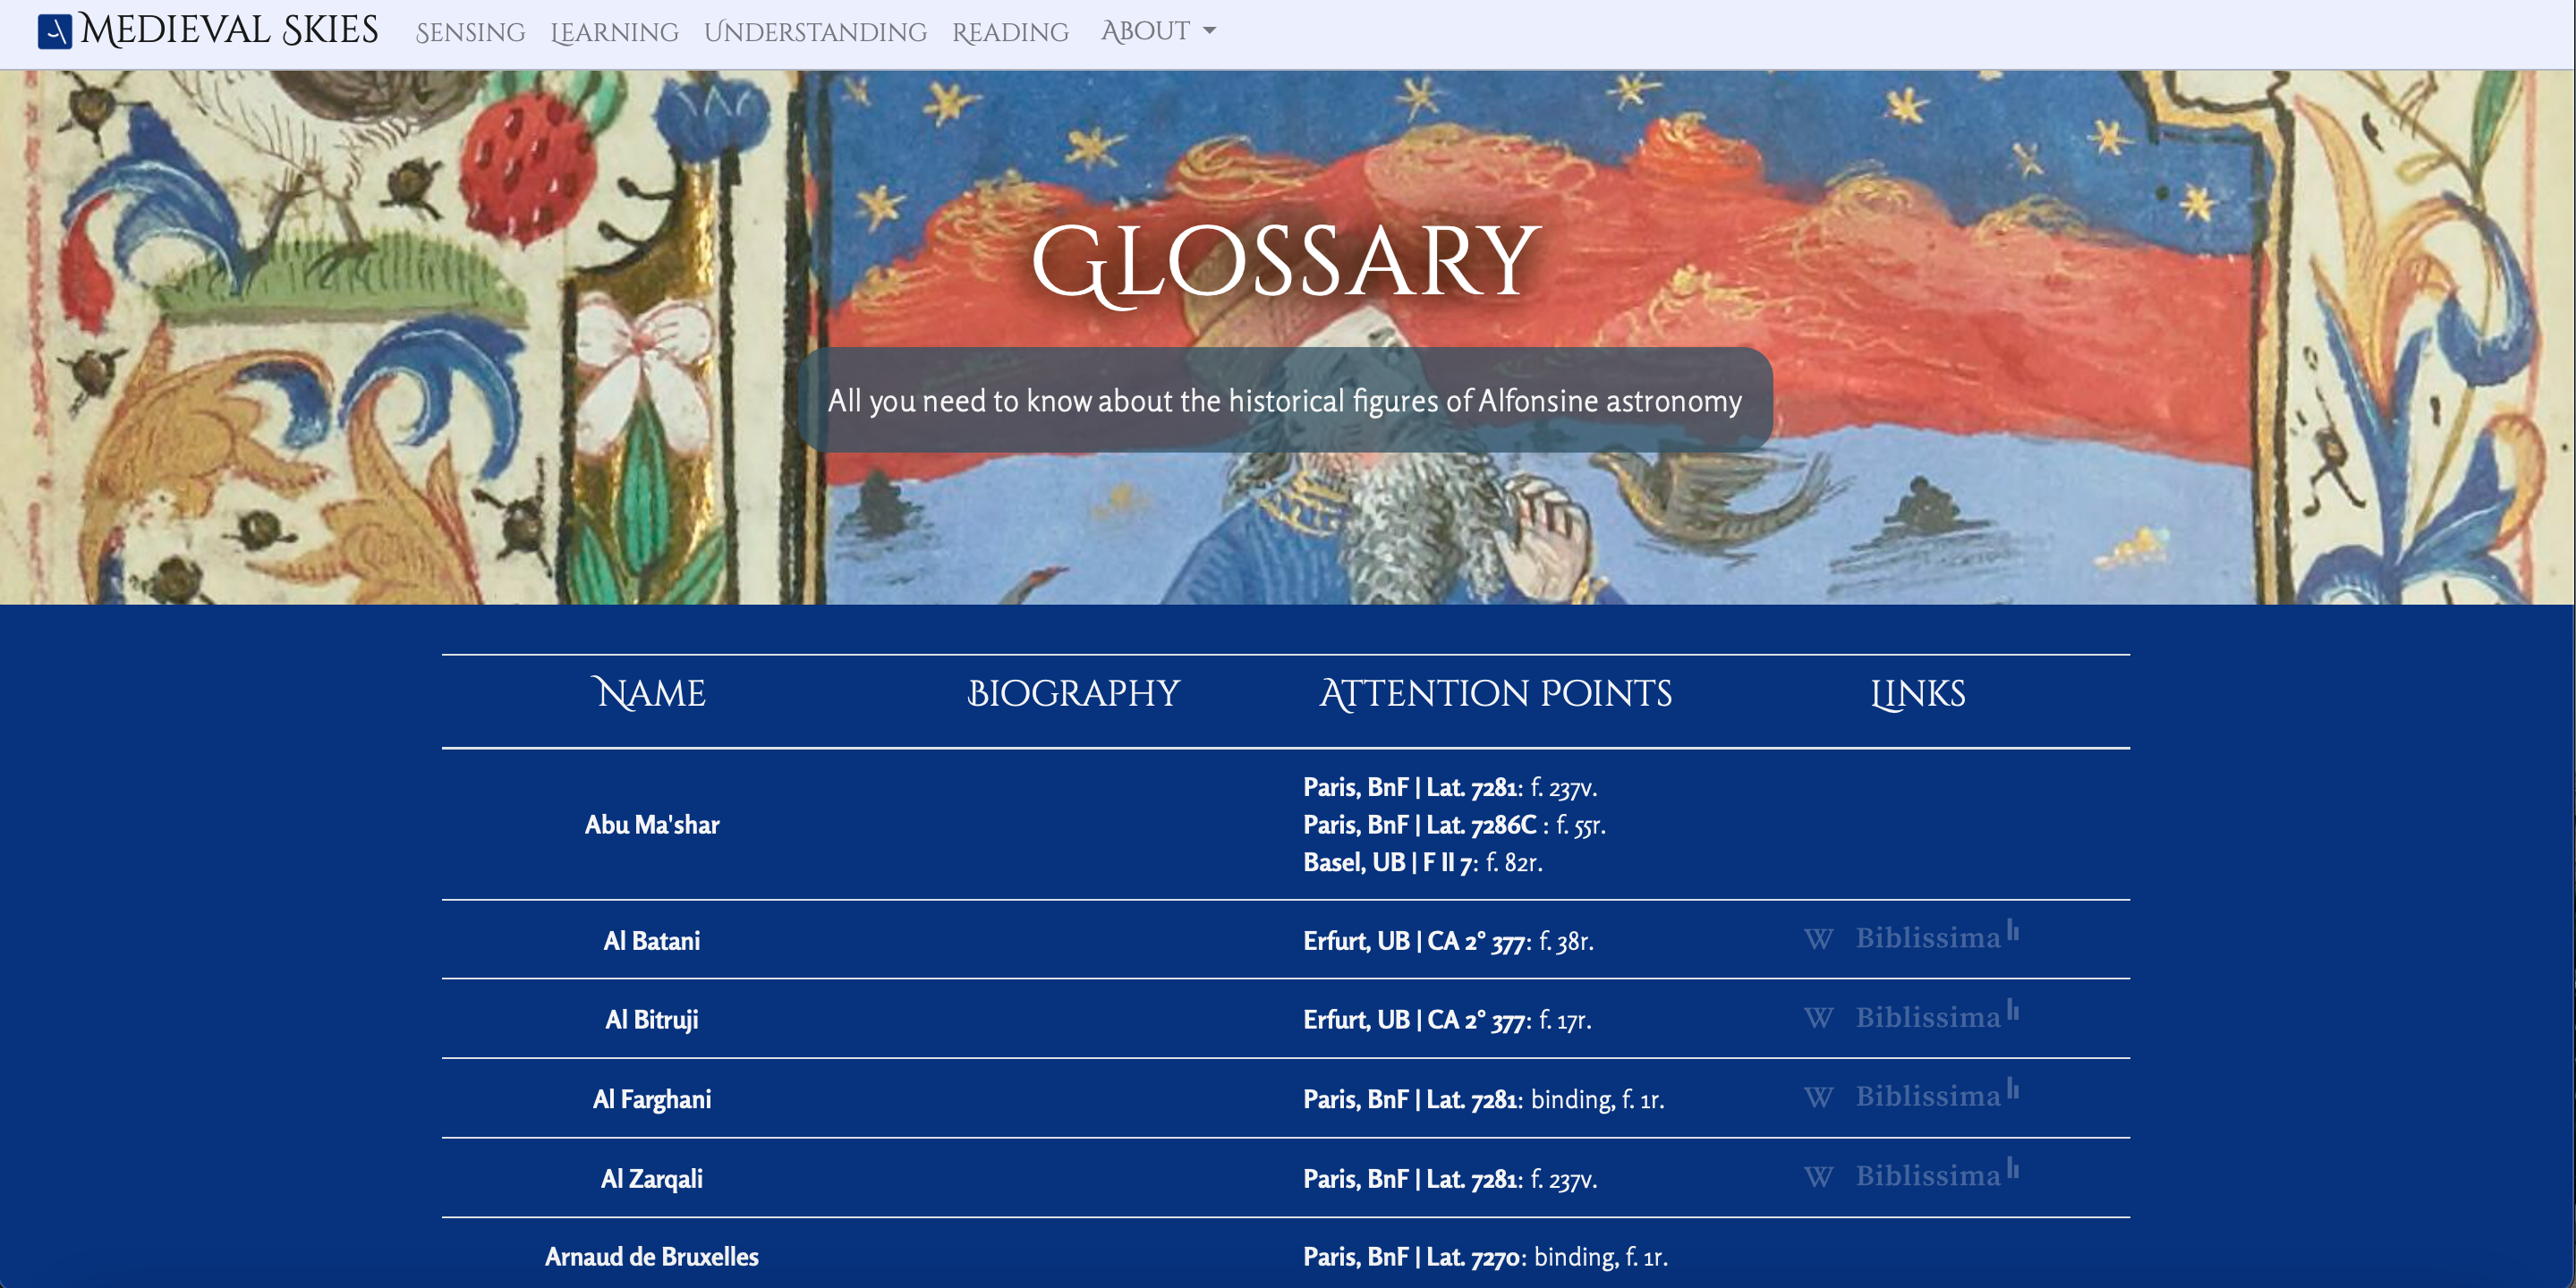
\includegraphics[width=\textwidth]{images/annexes/glossary-ordinateur.png}
    \end{subfigure}
    \begin{subfigure}[h]{0.6\textwidth}
        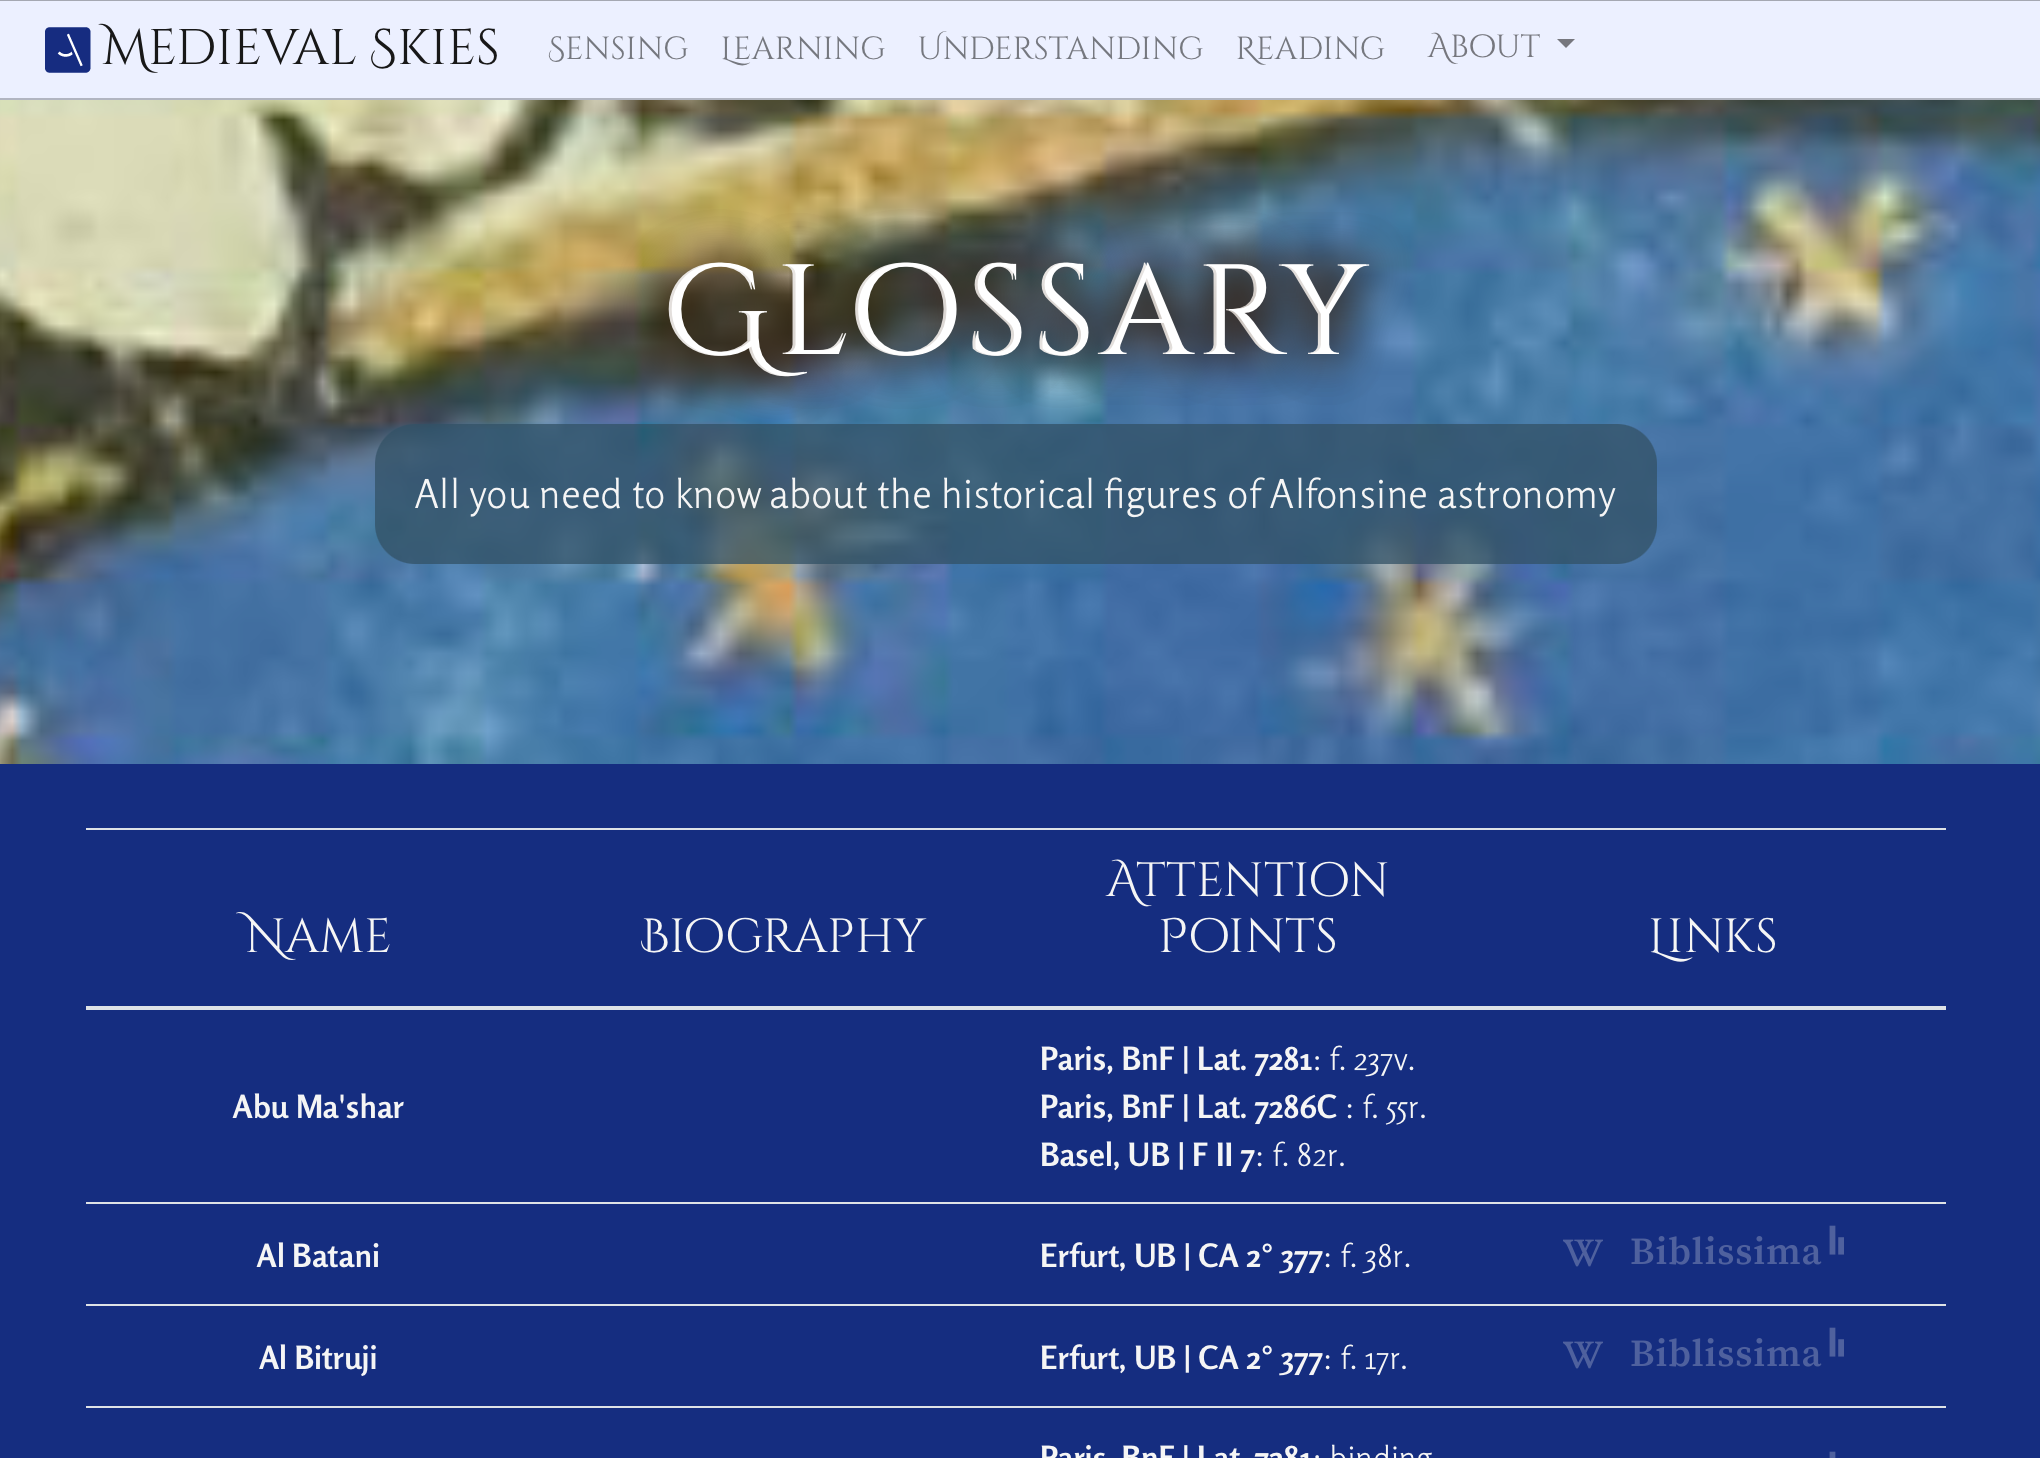
\includegraphics[width=\textwidth]{images/annexes/glossary-tablette.PNG}
    \end{subfigure}
    \begin{subfigure}[h]{0.3\textwidth}
        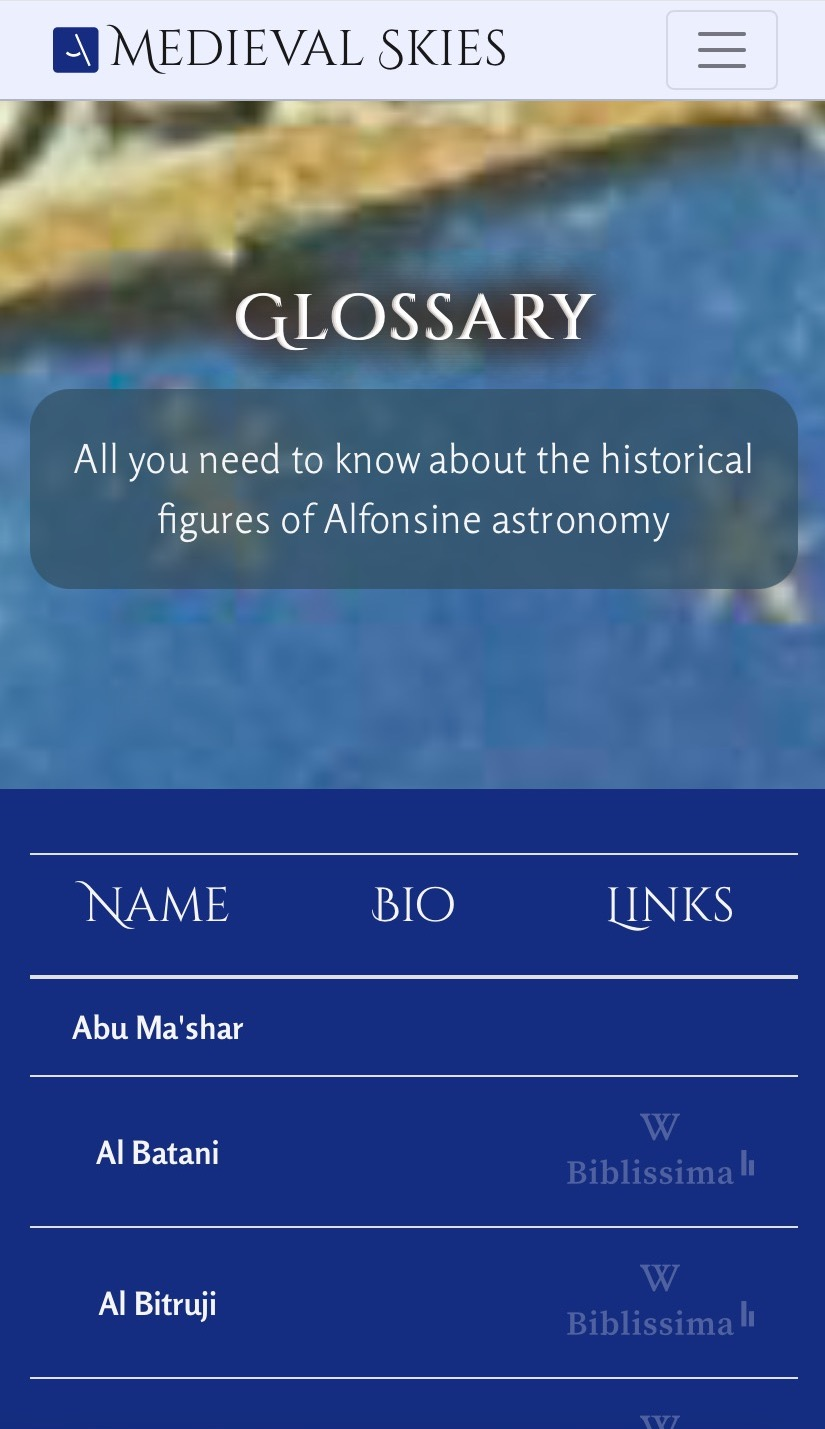
\includegraphics[width=\textwidth]{images/annexes/glossary-smartphone.jpeg}
    \end{subfigure}
    
    \caption{Pages \textit{Glossary} du site \textit{Medieval skies under(book)cover} sur un écran d'ordinateur, de tablette et de \textit{smartphone}}
    \end{figure}

% index à mettre ici si index	
%	\printindex

%\printglossaries

%imprimer séparément les deux listes
%\printglossary
\printglossary[type=\acronymtype]

% si figures
\listoffigures


\tableofcontents
	
\end{document}